\documentclass[12pt]{article}
\usepackage{preamble}

\pagestyle{fancy}
\fancyhead[LO,LE]{Математическая статистика}
\fancyhead[RO,RE]{Лекции Блаженова А. В.}

\fancyfoot[L]{\scriptsize исходники найдутся тут: \\ \url{https://github.com/pelmesh619/itmo_conspects} \Cat}

\renewcommand{\thesection}{}

\begin{document}

    \tableofcontents
    \clearpage

    % begin mathstat_2025_02_11.tex





\section{Лекция 1.}

Теория вероятности изучает характеристику случайных величин, тогда как математическая статистика решает обратную задачу

Допустим, что у нас есть случайная величина, по ней мы можем найти матожидание, моменты и оценить,
какое распределение имеет случайная величина. 

\subsection{Выборки}

\Def \textbf{Выборка} - набор данных, полученных в ходе экспериментов. Тогда количество экспериментов $n$ - объем Выборки

\Defs \textbf{Генеральной совокупностью} называются все результаты проведенных экспериментов

\Defs \textbf{Выборочной совокупностью} называются наблюдаемые данные экспериментов

Не все данные экспериментов мы можем наблюдать, например, выборы, тогда опросы голосовавших - выборочная совокупность, а
результаты выборов - генеральная. Очевидно, что выборочная и генеральная совокупности могут иметь различные распределения.

\Defs Выборка называется \textbf{репрезентативной}, если ее распределение близко к распределению генеральной совокупностью

Пример - \href{https://ru.wikipedia.org/wiki/%D0%A1%D0%B8%D1%81%D1%82%D0%B5%D0%BC%D0%B0%D1%82%D0%B8%D1%87%D0%B5%D1%81%D0%BA%D0%B0%D1%8F_%D0%BE%D1%88%D0%B8%D0%B1%D0%BA%D0%B0_%D0%B2%D1%8B%D0%B6%D0%B8%D0%B2%D1%88%D0%B5%D0%B3%D0%BE}{ошибка выжившего}. Во время Второй Мировой стал вопрос, в каких местах стоит бронировать корпус самолета. Самолеты 
возвращались с пулевыми отверстиям, и интуитивно казалось, что стоит бронировать те места, которые больше
всего пострадали. Однако не были учтены те самолеты, которые не вернулись, а те, которые выжили, выжили благодаря тому, что были 
прострелены в нелетальных местах, поэтому было принято решение бронировать фюзеляж в менее пострадавших местах

В дальнейшем считаем, что все выборки репрезентативны

\DefN{1} Выборкой объема $n$ называется набор из $n$ экспериментаных данных $\vec{X} = (x_1, x_2, \dots, x_n)$ (апостериорное определение)

\DefNs{2} Выборкой объема $n$ называется набор из $n$ независимых одинаково распределенных случайных
величин $\vec{X} = (X_1, X_2, \dots, X_n)$ (априорное определение)

\subsection{Выборочные характеристики}

Можно выборку рассматривать как дискретную случайную величину с одинаковыми вероятностями $p_i = \frac{1}{n}$
и вычислить для нее математическое ожидание, дисперсию и функцию распределения

\Def Выборочным средним $\overline{x}$ называется величина $\overline{x} = \frac{1}{n} \sum_{i = 1}^n X_i$

\Defs Выборочной дисперсией $D^*$ называется величина $D^* = \frac{1}{n} \sum_{i = 1}^n (X_i - \overline{x})^2$ (или $D^* = \frac{1}{n} \sum_{i = 1}^n X_i^2 - \overline{x}^2$)

По закону больших чисел выборочное среднее будет сходиться к матожиданию

\Defs Исправленной дисперсией называется величина $S^2 = \frac{n}{n - 1} D^* = \frac{1}{n - 1}\sum_{i = 1}^n (X_i - \overline{x})^2$

\hypertarget{selective_distribution_function}{}

\Def Выборочной функцией распределения $F^*(x)$ называется функция $F^*(x) = \frac{\text{число данных } x_i < x}{n}$

\begin{MyTheorem}
    \Ths Выборочная функция распределения поточечно сходится к теоретической функции распределения:

    \[\forall y \in \Real F^*(y) \overset{p}{\longrightarrow} F(y)\]
\end{MyTheorem}

\begin{MyProof}
    $F(y) = P(X < y)$

    $F^*_y = \frac{1}{n} \sum_{i = 1}^n I(X_i < y) \underset{\text{по ЗБЧ}}{\overset{p}{\longrightarrow}} EI(X_i < y) = P(X_i < y) = 
    P(X_1 < y) = F_{X_1}(y)$
\end{MyProof}

Усилим теорему

\begin{MyTheorem}
    \ThNs{Гливенко-Кантелли} $\sup_{x \in \Real} |F^*(x) - F(x)| \overset{p}{\longrightarrow} 0$
\end{MyTheorem}

\begin{MyTheorem}
    \ThNs{Колмогорова} $\sqrt{n} \sup_{x \in \Real} |F^*(x) - F(x)| \rightrightarrows K$ - распределение Колмогорова с 
    функцией распределения $F_K(x) = \sum_{j = -\infty}^{\infty} (-1)^j e^{-2 j^2 x^2}, \ x \in [0;\infty)$
\end{MyTheorem}

\hypertarget{initial_data_processing}{}

\subsection{Начальная обработка статданных}

\begin{enumerate}
    \item Ранжирование данных - упорядочиваем выборки по возрастанию. В результате получаем вариационный ряд $\vec{X} = (X_{(1)}, X_{(2)}, \dots, X_{(n)})$

    $X_{(1)} = \min X_i; \quad X_{(n)} = \max X_i$

    $X_{(i)} = i$-ая порядковая статистика

    \item Объединим повторяющиеся данные - получаем т.н. частотный вариационный ряд

    \begin{tabular}{c|c|c|c|c}
        $X_i$ & $X_{(1)}$ & \dots & $X_{(r)}$ & $\sum$ \\ 
        \hline
        $n_i$ & $n_1$ & \dots & $n_r$ & $n$ \\ 
    \end{tabular}

    Иногда часть данных отбрасывается сверху и снизу (по 5, по 10, по 5\% и так далее), чтобы сделать выборку репрезентативной

    Тогда $\overline{x} = \frac{1}{n} \sum X_i n_i$, $D^* = \frac{1}{n} \sum (X_i - \overline{x})^2 n_i$
    
    \item Чтобы уменьшить количество вычислений или сделать гистограмму, делают интервальный вариационный ряд: 
    разбиваем данные на интервалы и считаем, сколько данных $n_i$ попало в интервал. 

    Тогда $n_i$ - частота интервала $A_i$

    Есть два основные способа разбиения на интервалы: 

    \begin{enumerate}
        \item Интервалы одинаковой длины
        \item Равнонаполненные интервалы (в каждом интервале примерно одинаковое количество данных)
    \end{enumerate}

    Число интервалов $K$ такое, что $\frac{K(n)}{n} \longrightarrow 0$ и $K(n) \underset{n \to \infty}{\longrightarrow} \infty$

    Обычно применяют формулу Стерджесса $K \approx 1 + \log_2 n$ или $K \approx \sqrt[3]{n}$

    Пусть получили интервальный вариационный ряд

    \begin{tabular}{c|c|c|c|c|c}
        интервалы & $[a_0; a_1)$ & $[a_1; a_2)$ & \dots & $[a_{K - 1}; a_K]$ & $\sum$ \\ 
        \hline
        частоты & $n_1$ & $n_2$ & \dots & $n_K$ & $n$ \\ 
    \end{tabular}

\end{enumerate}

\subsection{Геометрическая интерпретация данных}

% https://www.geogebra.org/calculator/rcgr7r9f

\begin{itemize}
    \item Гистограмма

    Строится ступенчатая фигура из прямоугольников, основание $i$-ого прямоугольника - интервал, 
    высота прямоугольника - $\frac{n_i}{n l_i}$, где $l_i$ - длина интервала

    \begin{center}
        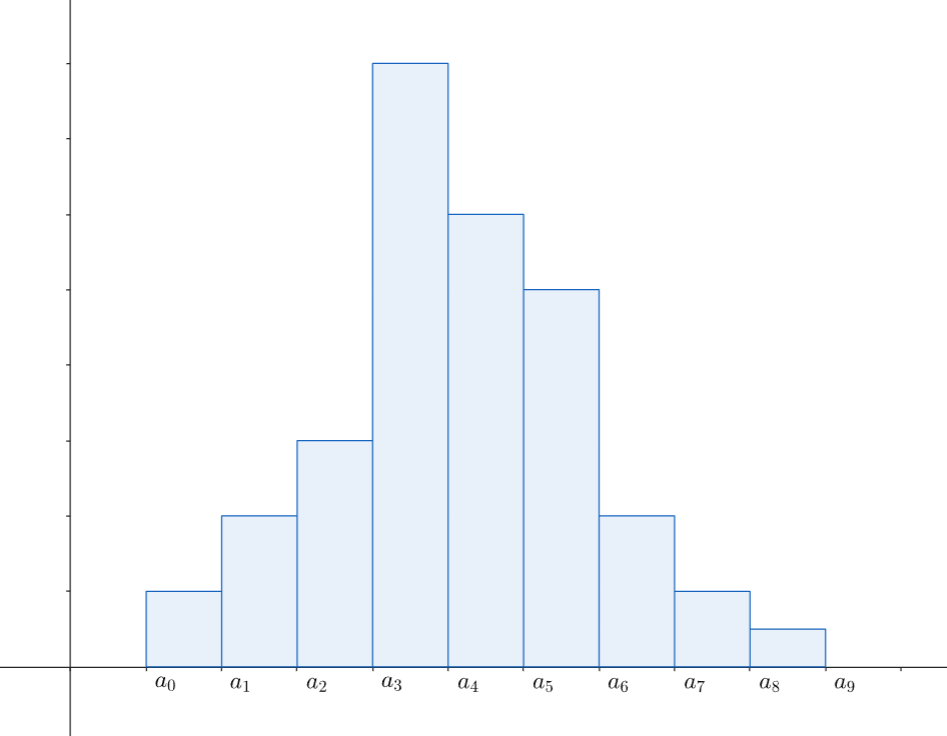
\includegraphics[width=0.7\textwidth]{mathstat/images/mathstat_2025_02_11_1}
    \end{center}

    Визуально можно сделать гипотезу, как ведет себя распределение. 

    \begin{MyTheorem}
        \Ths Гистограмма поточечно сходится к теоретической плотности
    \end{MyTheorem}

    \item Полигон

    На оси абсцисс отмечаем значения частотного вариационного ряда, по оси ординат - их частоты. 
    Получившиеся точки соединяем отрезками

    \begin{center}
        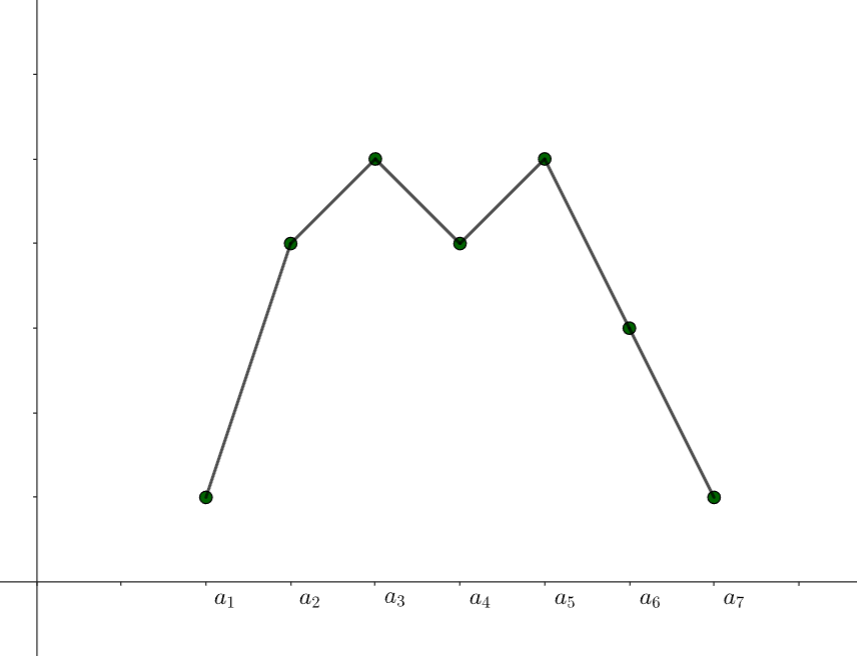
\includegraphics[width=0.7\textwidth]{mathstat/images/mathstat_2025_02_11_2}
    \end{center}

    \item Выборочная функция распределения

    На основе таблицы строится график функции распределения

    \begin{center}
        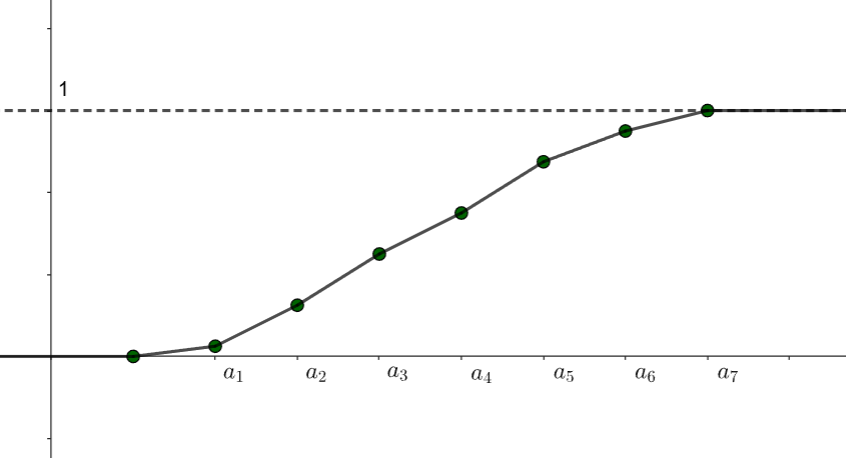
\includegraphics[width=0.7\textwidth]{mathstat/images/mathstat_2025_02_11_3}
    \end{center}

    Она может быть ступенчатой, ломаной или соединена по усмотрению

\end{itemize}





% end mathstat_2025_02_11.tex

% begin mathstat_2025_02_18.tex





\section{Лекция 2.}

\subsection{Точечная оценка}

\hypertarget{point_estimation}{}

Пусть имеется выборка $\vec{X} = (X_1, X_2, \dots, X_n)$ объемом $n$

Пусть требуется найти приближенную оценку $\theta^*$ неизвестного параметра $\theta$

Находим ее при помощи некоторой функции обработки данных $\theta^* = \theta^*(X_1, \dots, X_n)$

\Def Такая функция называется статистикой

\Defs А оценка $\theta^*$ называется точечной оценкой

\subsubsection{Свойство точечных оценок}

\begin{enumerate}
    \item Состоятельность

    \Defs Статистика $\theta^* = \theta^*(X_1, \dots, X_n)$ неизвестного параметра называется
    состоятельной, если $\theta^* \overset{p}{\longrightarrow} \theta$ при $n \to \infty$

    \mediumvspace

    \item Несмещенность

    \Defs Оценка $\theta^*$ параметра $\theta$ называется несмещенной, если 
    математическое ожидание $E \theta^* = \theta$
    
    \Notas Оценка $\theta^*$ называется асимптотически несмещенной, если 
    $E \theta^* \overset{p}{\longrightarrow} \theta$ при $n \to \infty$

    \mediumvspace

    \item Эффективность 

    \Defs Оценка $\theta^*_1$ не хуже $\theta^*_2$, если $E (\theta^*_1 - \theta)^2 \leq E (\theta^*_2 - \theta)^2$.
    Или, если $\theta^*_1$ и $\theta^*_2$ несмещенные, то $D \theta^*_1 \leq D \theta^*_2$

    \Defs Оценка $\theta^*$ называется эффективной, если она не хуже всех остальных оценок

    \Notas Не существует эффективной оценки в классе всех возможных оценок

    \begin{MyTheorem}
        \Ths В классе несмещенных оценок существует эффективная оценка
    \end{MyTheorem}

    \mediumvspace

    \item Асимптотическая нормальность

    \Defs Оценка $\theta^*$ параметра $\theta$ называется асимптотически нормальной, если 
    $\sqrt{n} (\theta^* - \theta) \rightrightarrows N(0, \sigma^2 (\theta))$ при $n \to \infty$
    
\end{enumerate}

\subsection{Точечные оценки моментов}

\hypertarget{moments_point_estimation}{}

\Def Выборочным средним $\overline{x}$ называется величина $\overline{x} = \frac{1}{n} \sum_{i = 1}^n X_i$

\Defs Выборочной дисперсией $D^*$ называется величина $D^* = \frac{1}{n} \sum_{i = 1}^n (X_i - \overline{x})^2$

\Defs Исправленной дисперсией $S^2$ называется величина $S^2 = \frac{n}{n - 1} D^* = \frac{1}{n - 1} \sum_{i = 1}^n (X_i - \overline{x})^2$

\Defs Выборочным средним квадратическим отклонением называется величина $\sigma^* = \sqrt{D^*}$

\Defs Исправленным средним квадратическим отклонением называется величина $S = \sqrt{S^2}$

\Defs Выборочным $k$-ым моментом называется величина $\overline{x^k} = \frac{1}{n} \sum_{i = 1}^n X_i^k$

\Defs Модой $\mathrm{Mo}^*$ называется варианта $x_k$ с наибольшей частотой $n_k = \max_i (n_1, n_2, \dots, n_m)$

\Defs Выборочной медианой $\mathrm{Me}^*$ называется варианта $x_i$ в середине вариационного ряда $\begin{cases}\mathrm{Me}^* = 
X_{(k)}, & \text{если } n = 2k - 1 \\ \frac{X_{(k)} + X_{(k + 1)}}{2}, & \text{если } n = 2k\end{cases}$

\begin{MyTheorem}
    \Ths $\overline{x}$ - состоятельная несмещенная оценка теоретического матожидания $EX = a$

    1) $E \overline{x} = a$

    2) $\overline{x} \overset{p}{\longrightarrow} a$ при $n \to \infty$
\end{MyTheorem}

\begin{MyProof}
    1) $E \overline{x} = E\left(\frac{X_1 + \dots + X_n}{n}\right) = \frac{1}{n} \sum_{i = 1}^n E X_i = 
    \frac{1}{n} n E X_1 = E X_1 = a$

    2) $\overline{x} = \frac{\overline{x}_1 + \dots + \overline{x}_n}{n} \overset{p}{\longrightarrow} a$ 
    согласно Закону Больших Чисел
\end{MyProof}

\Nota Если второй момент конечен, то $\overline{x}$ - асимптотически нормальная оценка. По ЦПТ $\frac{S_n - n E X_1}{\sqrt{n} \sqrt{D X_1}} = \sqrt{n} \frac{\overline{x} - E X_1}{\sqrt{D X_1}} \rightrightarrows N(0, 1)$
или $\sqrt{n} (\overline{x} - E X_1) \rightrightarrows N(0; D X_1)$

\begin{MyTheorem}
    \Ths Выборочный $k$-ый момент является состоятельной несмещенной оценкой теоретического $k$-ого момента

    1) $\overline{E X^k} = E X^k$

    2) $\overline{X^k} \overset{p}{\longrightarrow} X^k$
\end{MyTheorem}

Это следует из предыдущей теоремы, если взять $X^k$ вместо $X$

\begin{MyTheorem}
    \Ths Выборочная дисперсия $D^*$ и исправленная дисперсия $S^2$ являются состоятельными оценками теоретической дисперсией, при этом $D^*$ - смещенная оценка, а
    $S^2$ - несмещенная оценка
\end{MyTheorem}

\begin{MyProof}
    Заметим, что $D^* = \overline{X^2} - \overline{X}^2$

    $E D^* = E(\overline{X^2} - \overline{X}^2) = E\overline{X^2} - E (\overline{X}^2) = 
    E X^2 - E (\overline{X}^2)$

    Так как $D \overline{X} = E(\overline{X^2}) - (E \overline{X})^2$, то $E X^2 - E (\overline{X}^2) = 
    E X^2 - ((E\overline{X})^2 + D\overline{X}) = (E X^2 - EX) - D\overline{X} = D X - D \overline{X} = D X - D \left(\frac{X_1 + \dots + X_n}{n}\right) = 
    DX - \frac{1}{n^2} \sum_{i = 1}^n D X_i = DX - \frac{1}{n^2} n D X_1 = DX - \frac{1}{n} DX = \frac{n - 1}{n} DX$, то есть $D^*$ - смещенная вниз оценка

    $E S^2 = E(\frac{n}{n - 1} D^*) = \frac{n}{n - 1} \frac{n - 1}{n} DX = DX \Longrightarrow S^2$ - несмещенная оценка 

    2. $D^* = \overline{X^2} - \overline{X}^2 \overset{p}{\longrightarrow} E X^2 - (E X)^2 = DX$ - состоятельная оценка

    $S^2 = \frac{n}{n - 1} D^* \overset{p}{\longrightarrow} DX$
\end{MyProof}

\Nota Отсюда видим, что выборочная дисперсия - асимптотически несмещенная оценка. Поэтому при большом (обычно не меньше 100) объеме выборке можно
считать обычную выборочную дисперсию

\subsection{Метод моментов (Пирсона)}

\hypertarget{method_of_moments}{}

Постановка задачи: пусть имеется выборка объема $n$ неизвестного распределения, но известного типа,
которое задается $k$ параметрами: $\theta = (\theta_1, \theta_2, \dots, \theta_k)$. Требуется дать оценки данным
неизвестным параметрам

Идея метода состоит в том, что сначала находим оценки $k$ моментов, а затем с помощью теоретических формул
из теории вероятности даем оценки этих параметров

Пусть $\vec{X}$ - выборка из абсолютно непрерывного распределения $F_\theta$ с плотностью известного типа, 
которая задается $k$ параметрами $f_\theta (x, \theta_1, \dots, \theta_k)$

Тогда теоретические моменты находим по формуле $m_i = \int_{-\infty}^{\infty} x^i f_\theta (x, \theta_1, \dots, \theta_k) dx = h_i(\theta_1, \dots, \theta_n)$

Получаем систему из $k$ уравнений с $k$ неизвестными. В эти уравнения подставляем найденные оценки
моментов и, решая получившуюся систему уравнений, находим нужные оценки параметров

$\begin{cases}
    \overline{x} = h_1(\theta_1^*, \dots, \theta_n^*) \\ 
    \overline{x^2} = h_2(\theta_1^*, \dots, \theta_n^*) \\ 
    \dots \\
    \overline{x^k} = h_k(\theta_1^*, \dots, \theta_n^*) \\ 
\end{cases}$

\Nota Оценки по методу моментов как правило состоятельные, но часто смещенные

\Ex Пусть $X \in U(a, b)$. Обработав статданные, нашли оценки первого и второго моментов:

$\overline{x} = 2.25; \overline{x^2} = 6.75$

Найти оценки параметров $a^*, b^*$

Плотность равномерного распределения $f_{(a, b)} (x) = \begin{cases}0, & x < a \\ \frac{1}{b - a} & a \leq x \leq b, \\ 0, x > b\end{cases}$

$EX = \int_a^b x \frac{1}{b - a} dx = \frac{a + b}{2}$

$EX = \int_a^b x^2 \frac{1}{b - a} dx = \frac{a^2 + ab + b^2}{3}$

\mediumvspace

Получаем:

$\begin{cases}
    \overline{x} = \frac{a^* + b^*}{2} \\ 
    \overline{x^2} = \frac{a^*^2 + a^* b^* + b^*^2}{3} \\ 
\end{cases} \Longleftrightarrow \begin{cases}
    a^* + b^* = 4.5 \\ 
    a^*^2 + a^* b^* + b^*^2 = 20.25 \\ 
\end{cases} \Longleftrightarrow \begin{cases}
    a^* + b^* = 4.5 \\ 
    a^* b^* = 0 \\ 
\end{cases} \Longleftrightarrow \begin{cases}
    a^* = 0 \\ 
    b^* = 4.5 \\ 
\end{cases}$




% end mathstat_2025_02_18.tex

% begin mathstat_2025_02_25.tex





\section{Лекция 3.}

\subsection{Метод максимального правдоподобия}

\hypertarget{maximum_likelihood_estimation}{}

Пусть имеется выборка $\vec{X} = (X_1, \dots, X_n)$ из распределения известного типа, определяемого неизвестными параметрами 
$\theta = (\theta_1, \dots, \theta_n)$

Идея метода состоит в следующем: подбираем параметры таким образом, чтобы вероятность получения
данной выборки при случайном эксперименте была наибольшей.

Если распределение дискретное, то $P_{\theta} (X_1 = x_1, X_2 = x_2, \dots, X_n = x_n) = P(X_1 = x_1) \dots P(X_n = x_n)$

\Def Функцией правдоподобия $L(\vec{X}, \theta)$ называется функция $L(\vec{X}, \theta) = P(X_1 = x_1) \dots P(X_n = x_n) = \prod_{i = 1}^n P(X_i = x_i)$ при дискретном распределении

и $L(\vec{X}, \theta) = f_\theta(x_1) \dots f_\theta(x_n) = \prod_{i = 1}^n f_\theta(x_i)$ в абсолютно непрерывном распределении

\Def Логарифмической функцией правдоподобия называется функция $\ln L(\vec{X}, \theta)$

\Nota Так как $y = \ln x$ возврастающая функция, точки максимума совпадают, а такую функцию правдоподобия становится легче дифференцировать

\Def Оценкой максимального правдоподобия $\hat{\theta}$ называется значение $\theta$, при котором функция правдоподобия 
$L(\vec{X}, \theta)$ достигает наибольшего значения (при фиксированных значениях выборки)

\ExN{1} Пусть $\vec{X} = (X_1, \dots, X_n)$ - выборка из распределения Пуассона $\Pi_\lambda$ с неизвестным $\lambda > 0$

\Mem Для распределения Пуассона $P(X = x_i) = \frac{\lambda^{x_i}}{x_i!} e^{-\lambda}$

Получаем функцию максимального правдоподобия $L(\vec{X}, \lambda) = \prod_{i = 1}^n \frac{\lambda^{x_i}}{x_i!} e^{-\lambda} = 
\frac{\lambda^{\sum_{i = 1}^n x_i}}{\prod_{i = 1}^n x_i!} e^{-n\lambda} = \frac{\lambda^{n \overline{x}}}{\prod_{i = 1}^n x_i!} e^{-n\lambda}$

$\ln L(\vec{X}, \lambda) = n \overline{x} \ln \lambda - \ln \prod_{i = 1}^n x_i! - n\lambda$

$\frac{\partial \ln L}{\partial \lambda} = \frac{n \overline{x}}{\lambda} - n = 0 \Longrightarrow \hat{\lambda} = \overline{x}$ - оценка максимального правдоподобия

Убедимся, что этот экстремум - максимум: $\frac{\partial^2 \ln L}{\partial \lambda^2} = -\frac{n \overline{x}}{\lambda} < 0 \Longrightarrow \hat{\lambda} = \overline{x}$ - точка максимума

\ExN{2} Пусть $(X_1, \dots, X_n)$ из $N(a, \sigma^2)$

$f_{a, \sigma^2} (x) = \frac{1}{\sigma \sqrt{2\pi}} e^{-\frac{(x - a)^2}{2\sigma^2}}$

$L(\vec{X}, a, \sigma^2) = \prod_{i = 1}^n \frac{1}{\sigma \sqrt{2\pi}} e^{-\frac{(x_i - a)^2}{2\sigma^2}} = 
\frac{1}{\sigma^n (2\pi)^{\frac{n}{2}}} e^{-\frac{\sum_{i = 1}^n (x_i - a)^2}{2\sigma^2}}$

$\ln L(\vec{X}, a, \sigma^2) = -n\ln \sigma - \frac{n}{2} \ln 2\pi - \frac{1}{2\sigma^2}\sum_{i = 1}^n (x_i - a)^2$

$\frac{\partial \ln L}{\partial a} = -\frac{1}{2\sigma^2} \sum_{i = 1}^n -2(x_i - a) = \frac{1}{\sigma^2} \sum_{i = 1}^n (x_i - a) = \frac{n\overline{x} - na}{\sigma^2}$

$\frac{\partial \ln L}{\partial \sigma} = -\frac{n}{\sigma} - \sum_{i = 1}^n (x_i - a)^2 \frac{1}{2} \cdot (-2) \cdot \sigma^{-3} = \frac{1}{\sigma^3} \sum_{i = 1}^n (x_i - a)^2 - \frac{n}{\sigma}$

$\begin{cases}
    \frac{n\overline{x} - na}{\sigma^2} = 0 \\
    \frac{1}{\sigma^3} \sum_{i = 1}^n (x_i - a)^2 - \frac{n}{\sigma} = 0
\end{cases} \Longrightarrow \begin{cases}
    \hat{a} = \overline{x} \\
    \widehat{\sigma^2} = \frac{1}{n} \sum_{i = 1}^n (x_i - a)^2 = D^*
\end{cases} $

\ExN{3} Пусть $(X_1, \dots, X_n)$ из $U(0, \theta)$. Найти оценку $\theta$ этого распределения.

Воспользуемся методом моментов:

$EX = \frac{a + b}{2} = \frac{\theta}{2} \Longrightarrow \overline{x} = \frac{\theta^*}{2} \Longrightarrow \theta^* = 2\overline{x}$

Воспользуемся методом максимального правдоподобия:

$f_\theta = \begin{cases}0, & x < 0 \\ \frac{1}{\theta}, & 0 \leq x \leq \theta \\ 0, & x > \theta \end{cases}$

$X_{(n)} = \max_i (X_1, \dots, X_n)$

$L(\vec{X}, \theta) = \prod_{i = 1}^n f_\theta (x_i) = 
\begin{cases}
    0, & \text{если } \theta < X_{(n)} \\ 
    \frac{1}{\theta^n}, & \text{если } \theta \geq X_{(n)}
\end{cases}$

$L(\vec{X}, \theta)$ достигает наибольшего значения при наименьшем значении $\theta^n$, то есть при $\hat{\theta} = X_{(n)}$

Сравним оценки:

$\theta^* = 2 \overline{x}$ - несмещенная оценка, так как $E\theta^* = 2E\overline{x} = 2E X = \theta$

$E(\theta^* - \theta)^2 = D\theta^* = D2\overline{x} = 4D\overline{x} = 4\frac{Dx}{n} = \frac{4}{n}\frac{\theta^2}{12} = \frac{\theta^2}{3n}$

Изучим распределение $X_{(n)}$: $F_{X_{(n)}}(x) = P(X_{(n)} < x) = P(X_1 < x, X_2 < x, \dots, X_n < x) = 
P(X_1 < x) \dots P(X_n < x) = F_{X_1}(x) \dots F_{X_n}(x) = F^n_{(x_1)}(x)$

$F_{X_1} (x) = \begin{cases}
    0, & x < 0 \\
    \frac{x}{\theta}, & 0 \leq x \leq \theta \\
    1, & x > \theta
\end{cases} \Longrightarrow F_{X_{(n)}}(x) = \begin{cases}
    0, & x < 0 \\
    \frac{x^n}{\theta^n}, & 0 \leq x \leq \theta \\
    1, & x > \theta
\end{cases} \Longrightarrow f_{X_{(n)}}(x) = \begin{cases}
    0, & x < 0 \\
    n\frac{x^{n - 1}}{\theta^n}, & 0 \leq x \leq \theta \\
    1, & x > \theta
\end{cases}$

$EX_{(n)} = \int_0^\theta x \cdot \frac{nx^{n - 1}}{\theta^n} dx = \frac{n}{\theta^n} \int_0^\theta x^n dx = \frac{n x^{n + 1}}{\theta^n (n + 1)} \Big|_0^\theta = 
\frac{n\theta}{n + 1}$ - смещенная вниз оценка

$\tilde{\theta} = \frac{n + 1}{n} X_{(n)}$ - несмещенная оценка (будем считать, что эффективность не изменилась)

$E\tilde{\theta}^2 = E(\frac{n + 1}{n} X_{(n)})^2 = \frac{(x + 1)^2}{n^2} E X_{(n)} = \frac{(n + 1)^2}{n^2} \int_0^\theta x^2 \frac{n x^{n - 1}}{\theta^n} dx = 
\frac{(n + 1)^2 \theta^2}{n (n + 2)}$

$D\tilde{\theta} = E\tilde{\theta}^2 - (E\tilde{\theta})^2 = \frac{\theta^2}{n(n + 2)}$

$D\tilde{\theta} = \frac{\theta^2}{n(n + 2)} < \frac{\theta^2}{3n} = D\theta^*$

Таким образом, оценка по методу правдоподобия сходится быстрее, чем оценка по методу моментов, поэтому она лучше

Отсюда следует, что при равномерном распределении выборочное среднее не является эффективной оценкой
для математического ожидания; вместо нее половина максимального элемента выборки будет лучше

\Nota Эффективной здесь будет несмещенная оценка $\frac{n + 1}{2n} X_{(n)}$

В общем случае для $U(a, b)$ будет такая эффективная оценка матожидания - $\frac{X_{(1)} + X_{(n)}}{2}$, длины интервала - $\frac{n + 1}{n - 1} (X_{(n)} - X_{(1)})$

\Nota При методе максимального правдоподобия обычно получаем состоятельные и эффективные оценки, но часто смещенные

\subsection{Неравенство Рао-Крамера}

Пусть $X \in F_\theta$ - семейство распределений с параметром $\theta \in \Real$

\Def Носителем семейства распределений $F_\theta$ называется множество $C \subset \Real$
такое, что $P(X \in C) = 1 \ \forall X \in F_\theta$

$f_\theta(x) = \begin{cases}
    \text{плотность } f_\theta(x) \text{ при непрерывном распределении} \\
    P_\theta(X = x) \text{ при дискретном распределении}
\end{cases}$

\hypertarget{fishers_information}{}

\Def Информацией Фишера $I(\theta)$ семейства распределений $F_\theta$ называется величина 
$I(\theta) = E\left(\frac{\partial}{\partial \theta} \ln f_\theta(X)\right)^2$ при условии, что
она существует

\Def Семейство распределений $F_\theta$ называется регулярным, если:

\begin{itemize}
    \item существует носитель $C$ семейства $F_\theta$ такой, что $\forall x \in C \ $ функция $\ln f_\theta(x)$ непрерывно дифференцируема по $\theta$
    \item информация Фишера $I(\theta)$ существует и непрерывна по $\theta$
\end{itemize}

\hypertarget{rao_kramer_inequality}{}

\begin{MyTheorem}
    \Ths Пусть $(X_1, \dots, X_n)$ - выборка объема $n$ из регулярного семейства $F_\theta$,

    $\theta^* = \theta^*(X_1, \dots, X_n)$ - несмещенная оценка параметра $\theta$, дисперсия которой
    $D\theta^*$ ограничена в любой замкнутой ограниченной области параметра $\theta$

    Тогда \fbox{$D\theta^* \geq \frac{1}{n I(\theta)}$}
\end{MyTheorem}

\underline{Следствие}: если при данных услових получили $D\theta^* = \frac{1}{n I(\theta)}$, то оценка $\theta^*$ является эффективной 
(то есть дальше улучшать уже некуда)

\Ex Пусть $(X_1, \dots, X_n)$ из $N(a, \sigma^2)$ (то есть $F_a = N(a, \sigma^2)$, $\sigma^2$ зафиксируем)

Проверим эффективность $a^* = \overline{x}$

Плотность $f_a(x) = \frac{1}{\sigma \sqrt{2\pi}} e^{-\frac{(x - a)^2}{2\sigma^2}}$, носитель - вся прямая $\Real$

$\ln f_a(x) = -\ln \sigma - \frac{1}{2} \ln 2\pi - \frac{(x - a)^2}{2\sigma^2}, \quad\quad a \in (-\infty, \infty)$

$\frac{\partial}{\partial a} \ln f_a(x) = \frac{1}{2\sigma^2} \cdot 2(x - a) = \frac{x - a}{\sigma^2}$ - непрерывна для всех $a \in \Real$

$I(a) = E\left(\frac{\partial}{\partial a} \ln f_a(X)\right)^2 = E\left(\frac{X - a}{\sigma^2}\right)^2 = \frac{1}{\sigma^4} E(X - a)^2 = \frac{E(X - EX)^2}{\sigma^4} = 
\frac{DX}{\sigma^4} = \frac{1}{\sigma^2}$ - непрерывна по $a$

Из этого следует, что $N(a, \sigma^2)$ - регулярное семейство относительно параметра $a$

$Da^* = D\overline{x} = \frac{DX}{n} = \frac{\sigma^2}{n}$ - ограничена по параметру $a$

По неравенству Рао-Крамера $Da^* = \frac{\sigma^2}{n} =\joinrel= \frac{1}{nI(a)} = \frac{1}{n} \sigma^2$; из 
этого следует, что $a^*$ - эффективная оценка параметра $a$

\Nota Аналогично можно показать, что $S^2$ - несмещенная эффективная оценка для параметра $\sigma^2$



% end mathstat_2025_02_25.tex

% begin mathstat_2025_03_04.tex





\section{Лекция 4.}

\subsection{Основные распределения математической статистики}

\Def Случайная величина имеет нормальное распределение $\xi \in N(a, \sigma^2)$ с параметрами $a$ и $\sigma^2$, если
ее плотность имеет вид $f_\xi(x) = \frac{1}{\sigma\sqrt{2\pi}} e^{-\frac{(x - a)^2}{2\sigma^2}}$

На практике нормальное распределение встречается чаще всего в силу ЦПТ

\Def Распределение $N(0, 1)$ с параметрами $a = 0, \sigma^2 = 1$ называется стандартным нормальным распределением. 
Его плотность равна $\varphi(x) = \frac{1}{\sqrt{2\pi}} e^{-\frac{x^2}{2}}$. 
В дальнейшем такую случайную величину будем называть стандартной нормалью

\underline{Свойства}

\begin{enumerate}
    \item $a = E\xi \qquad \sigma^2 = D\xi$

    \item Линейность: $\xi \in N(a, \sigma^2)$, то $\eta = b \xi + \gamma \in N(ab + \gamma, b^2 \sigma^2)$

    \item Стандартизация: Если $\xi \in N(a, \sigma^2)$, то $\eta = \frac{\xi - a}{\sigma} \in N(0, 1)$

    \item Устойчивость относительно суммирования: если $\xi_1 \in N(a_1, \sigma^2_1)$, $\xi_2 \in N(a_2, \sigma^2_2)$, независимы
    то $\xi_1 + \xi_2 \in N(a_1 + a_2, \sigma^2_1 + \sigma^2_2)$
\end{enumerate}

\subsubsection{Распределение \enquote{хи-квадрат}}

\Def Распределение \enquote{хи-квадрат} $H_n$ со степенями свободы $n$ называется распределение
суммы квадратов независимых стандартных нормальных величин: $\chi^2_n = X_1^2 + X_2^2 + \dots + X_n^2$, 
где $X \in N(0, 1)$ и независимы

\underline{Свойства}

\begin{enumerate}
    \item $E\chi^2_n = n$

    \begin{MyProof}
        Так как $\forall i \ X_i \in N(0, 1)$, то $E X_i^2 = D X_i^2 + (EX_i)^2 = 1 \Longrightarrow E(X_i^2 + \dots X_n^2) = \sum_{i = 1}^n E X_i^2 = n$
    \end{MyProof}

    \item Устойчивость относительно суммирования: если $X \in H_n$, $Y \in H_m$, независимы, то $X + Y \in H_{n + m}$ (по определению) 


    \item $\frac{\chi_k^2}{k} \overset{p}{\underset{k \to \infty}{\longrightarrow}} 1$ (по Закону Больших Чисел)
\end{enumerate}

\subsubsection{Распределение Стьюдента}

\Def Пусть $X_0, X_1, \dots, X_k$ - независимые стандартные нормальные величины. 
Распределением Стьюдента $T_k$ с $k$ степенями свободы называется распределение случайной величины 
$t_k = \frac{X_0}{\sqrt{\frac{1}{k} (X_1^2 + \dots + X_k^2)}} = \frac{X_0}{\sqrt{\frac{\chi_k^2}{k}}}$

\underline{Свойства}

\begin{enumerate}
    \item $Et_k = 0$ - в силу симметрии

    \item $t_k \rightrightarrows N(0, 1)$ (на практике при $k \geq 100$ распределение Стьюдента можно считать стандартным нормальным)
\end{enumerate}

\subsubsection{Распределение Фишера-Снедекера}

\Def Распределением Фишера-Снедекера $F_{n,m}$ (другое название - F-распределение) со степенями свободы $n$ и $m$ называется распределение случайной величины 
$f_{n,m} = \frac{\frac{\chi^2_n}{n}}{\frac{\chi^2_m}{m}}$, где $\chi_n^2$ и $\chi_m^2$ - независимые случайные величины с распределением \enquote{хи-квадрат}

\underline{Свойства}

\begin{enumerate}
    \item $E f_{n,m} = \frac{n}{n - 2}$

    \item $f_{n,m} \overset{p}{\underset{n, m \to \infty}{\longrightarrow}} 1$
\end{enumerate}


\subsection{Математическое ожидание и дисперсия случайного вектора}

Пусть $\vec X = \begin{pmatrix}X_1 \\ \vdots \\ X_n\end{pmatrix}$ - случайный вектор, 
где случайная величина $X_i$ - компонента (координата) случайного вектора

\Def Математическим ожидание случайного вектора называется вектор с координатами из математических ожиданий компонент: 
$E \vec X = \begin{pmatrix}E X_1 \\ \vdots \\ E X_n\end{pmatrix}$

\Def Дисперсией случайного вектора (или матрицей ковариаций) случайного вектора $\vec X$ называется
матрица $D \vec X = E (\vec X - E \vec X) (\vec X - E \vec X)^T$, состоящая из элементов $d_{ij} = \mathrm{cov} (X_i, X_j)$

\Notas На главной диагонали стоят дисперсии компонент: $d_{ii} = D X_i$

\Notas $D \vec X$ - симметричная положительно определенная матрица

\underline{Свойства}

\begin{enumerate}
    \item $E (A \vec X) = A E \vec X$

    \item $E (\vec X + \vec B) = E \vec X + \vec B$, где $\vec B$ - вектор чисел

    \item $D (A \vec X) = A \cdot D \vec X \cdot A^T$

    \item $D (\vec X + \vec B) = D \vec X$
\end{enumerate}

\subsection{Многомерное нормальное распределение}

\Def Пусть случайный вектор $\vec \xi = \begin{pmatrix}\xi_1 \\ \vdots \\ \xi_n\end{pmatrix}$ имеет вектор средних 
$\vec a = E \vec \xi$, $K$ - симметричная положительно определенная матрица. Вектор $\vec \xi$ 
имеет нормальное распределение в $\Real^n$ с параметрами $\vec a$ и $K$, если его плотность 
$f_{\vec \xi} (\vec X) = \frac{1}{\left(\sqrt{2\pi}\right)^n \sqrt{\det K}} e^{-\frac{1}{2} (\vec X - \vec a)^T K^{-1} (\vec X - \vec a)}$


\underline{Свойства}

\begin{enumerate}
    \item Матрица $K = D \vec \xi = \left(\mathrm{cov} (\xi_i, \xi_j)\right)$ - матрица ковариаций

    \item При $\vec a = \vec 0$ и $K = E$ имеем вектор из независимых стандартных нормальных величин

    \begin{MyProof}
        При $\vec a = \vec 0$ и $K = E$: $f_{\vec \xi} (X_1, \dots, X_n) = \frac{1}{\left(\sqrt{2\pi}\right)^n} 
        e^{-\frac{1}{2} \begin{pmatrix}X_1 & \dots & X_n\end{pmatrix} E \begin{pmatrix}X_1 & \dots & X_n\end{pmatrix}^T} = 
        \frac{1}{\left(\sqrt{2\pi}\right)^n} e^{-\frac{1}{2} (X_1^2 + \dots + X_n^2)} = 
        \frac{1}{\sqrt{2\pi}} e^{-\frac{1}{2} X_1^2} + \dots + \frac{1}{\sqrt{2\pi}} e^{-\frac{1}{2} X_n^2}$

        Так как плотность распалась на произведение плотностей стандартного нормального распределение, то все компоненты имеют стандартное нормальное распределение
    \end{MyProof}
\end{enumerate}

Далее вектор из независимых стандартных нормальных величин для краткости будем называть стандартным нормальным вектором

\begin{enumerate}
    \setcounter{enumi}{2}

    \item $\letsymbol \vec X$ - стандартный нормальный вектор, $B$ - невырожденная матрица, 
    тогда вектор $\vec Y = B \vec X + \vec a$ имеет многомерное нормальное распределение с параметрами $\vec a$ и $K = B B^T$

    \item $\letsymbol \vec Y \in N(\vec a, K)$. Тогда вектор $\vec X = B^{-1} (\vec Y - \vec a)$ - стандартный нормальный вектор, где $B = \sqrt{K}$

    \underline{Следствие}. Эквивалентное определение: Многомерное нормальное распределение - это то, которое получается из
    стандартного нормального вектора при помощи невырожденного преобразования и сдвига

    \item $\letsymbol \vec X$ - стандартный нормальный вектор, $C$ - ортогональная матрица. Тогда $\vec Y = C \vec X$ - стандартный нормальный вектор

    \begin{MyProof}
        Так как $C$ - ортогональная, то $C^T = C^{-1}$. Тогда по третьему свойству $K = C C^T = E$, а по второму свойству $\vec Y$ - стандартный нормальный вектор
    \end{MyProof}

    \item $\letsymbol$ случайный вектор $\xi \in N(\vec a, K)$.
    Тогда его координаты независимы тогда и только тогда, когда они не коррелированы (то есть матрица ковариаций $K$ диагональная)

    % какого распределения величины
    \underline{Следствие}. Если плотность совместного распределения случайных величин $\xi$ и $\eta$ ненулевая, то они независимы тогда и только тогда, 
    когда их коэффициент корреляции равен нулю
\end{enumerate}

\subsection{Многомерная центральная предельная теорема}

\begin{MyTheorem} 
    \Ths Среднее арифметическое независимых одинаково распределенных случайных векторов слабо сходится к многомерному нормальному распределению
\end{MyTheorem}

\subsection{Лемма Фишера}

\hypertarget{fishers_lemma}{}

\begin{MyTheorem}
    Пусть вектор $\vec X$ - стандартный нормальный вектор, $C$ - ортогональная матрица, $\vec Y = C \vec X$.
    Тогда $\forall 1 \leq k \leq n - 1 \ $ случайная величина $T(\vec X) = \sum_{i = 1}^n X_i^2 - Y_1^2 - Y_2^2 - \dots Y_k^2$ 
    не зависит от $Y_1, Y_2, \dots, Y_k$ и имеет распределение \enquote{хи-квадрат} со степенями свободы $n - k$
\end{MyTheorem}

\begin{MyProof}
    Так как $C$ - ортогональное преобразование, то $\|\vec X\| = \|\vec Y\|$, то есть $\sum_{i = 1}^n X^2_i = \sum_{i = 1}^n Y^2_i \Longrightarrow
    T(\vec X) = \sum_{i = 1}^n X_i^2 - Y_1^2 - Y_2^2 - \dots Y_k^2 = Y^2_{k + 1} + \dots + Y^2_{n}$

    Согласно свойству 5 $Y_i \in N(0, 1)$ и независимы, то по определению \enquote{хи-квадрат} $T(\vec X) \in H_{n - k}$ и не зависит от $Y_1, \dots, Y_k$
\end{MyProof}

\subsection{Основная теорема}

Эта теорема также известна как \href{https://tvims.nsu.ru/chernova/ms/lec/node37.html}{основное следствие леммы Фишера}

\begin{MyTheorem}
    \Ths Пусть $(X_1, \dots, X_n)$ - выборка из нормального распределения $N(a, \sigma^2)$, $\overline{x}$ - выборочное среднее, $S^2$ - исправленная дисперсия.

    Тогда справедливы следующие высказывания:

    \begin{enumerate}
        \item $\sqrt{n} \frac{\overline{x} - a}{\sigma} \in N(0, 1)$
        
        \item $\sum_{i = 1}^n \frac{(X_i - a)^2}{\sigma^2} \in H_n$
        
        \item $\sum_{i = 1}^n \frac{(X_i - \overline{x})^2}{\sigma^2} = \frac{n D^*}{\sigma^2} = \frac{(n - 1) S^2}{\sigma^2} \in H_{n - 1}$

        \item $\sqrt{n} \frac{\overline{x} - a}{S} \in T_{n - 1}$
        
        \item $\overline{x}$ и $S^2$ независимы
    \end{enumerate}
\end{MyTheorem}

\begin{MyProof}
    \begin{enumerate}
        \item Так как $X_i \in N(a, \sigma^2)$, то $\sum_{i = 1}^n X_i \in N(na, n\sigma^2) \Longrightarrow \overline{x} \in N\left(a, \frac{\sigma^2}{n}\right) \Longrightarrow
        \overline{x} - a \in N\left(0, \frac{\sigma^2}{n}\right) \Longrightarrow \frac{\sqrt{n}}{\sigma} (\overline{x} - a) \in N(0, 1)$

        \item Так как $X_i \in N(a, \sigma^2)$, то $\frac{X_i - a}{\sigma} \in N(0, 1)$ и $\sum_{i = 1}^n \frac{(X_i - a)^2}{\sigma^2} \in H_n$ по определению
        
        \item $\sum_{i = 1}^n \frac{(X_i - \overline{x})^2}{\sigma^2} = \sum_{i = 1}^n \left(\frac{X_i - a}{\sigma} - \frac{\overline{x} - a}{\sigma}\right)^2 = 
        \sum_{i = 1}^n (z_i - \overline{z})^2$, где $z_i = \frac{X_i - a}{\sigma} \in N(0, 1)$, $\overline{z} = \frac{1}{n} \sum_{i = 1}^n z_i = \frac{\sum_{i = 1}^n X_i - na}{\sigma} = \frac{\overline{x} - a}{\sigma}$

        Поэтому можно считать, что изначально $X_i \in N(0, 1)$

        $T(\vec X) = \sum_{i = 1}^n \left(X_i - \overline{x}\right)^2 = n D^* = n (\overline{x^2} - \overline{x}^2) = \sum_{i = 1}^n X_i^2 - n\overline{x}^2 = \sum_{i = 1}^n X_i^2 - Y_1^2$, где $Y_1 = \sqrt{n} \overline{x} = \frac{X_1}{\sqrt{n}} + \dots + \frac{X_n}{\sqrt{n}}$

        Строчка $\left(\frac{1}{\sqrt{n}}, \dots, \frac{1}{\sqrt{n}}\right)$ имеет длину 1, поэтому ее можно дополнить до ортогональной матрицы $C$, тогда $Y_1$ - первая компонента $\vec Y = C \vec X$, 
        и согласно лемме Фишера $T(\vec X) = \sum_{i = 1}^n (X_i - \overline{X})^2 \in H_{n - 1}$

        
        \setcounter{enumi}{4}
        \item Согласно лемме Фишера $T(\vec X) = (n - 1) S^2$ не зависит от $Y_1 = \sqrt{n} \overline{x} \Longrightarrow S^2 $ и $\overline{x}$ - независимы
          
        \setcounter{enumi}{3}
        \item $\sqrt{n} \frac{\overline{x} - a}{S} = \sqrt{n} \frac{\overline{x} - a}{\sigma} \cdot \frac{1}{\sqrt{\frac{S^2 (n - 1)}{\sigma^2}} \cdot \frac{1}{n - 1}} = \frac{\sqrt{n} \frac{\overline{x} - a}{\sigma}}{\frac{\chi^2_{n - 1}}{n - 1}}$

        Так как по пятому пункту числитель и знаменатель независимы, по определению получаем распределение Стьюдента
    \end{enumerate}
\end{MyProof}






% end mathstat_2025_03_04.tex

% begin mathstat_2025_03_11.tex





\section{Лекция 5.}

\subsection{Квантильное распределение}

Предполагаем, что распределение абсолютно непрерывное и $F(x)$ - функция распределения

\DefN{1} Число $t_\gamma$ называется квантилем распределения уровня $\gamma$, если значения
функции распределения $F(t_\gamma) = \gamma$ или $P(X < t_\gamma) = \gamma$ ($t_\gamma = F^{-1}(\gamma)$)

% https://www.geogebra.org/calculator/ezemup66

\begin{center}
    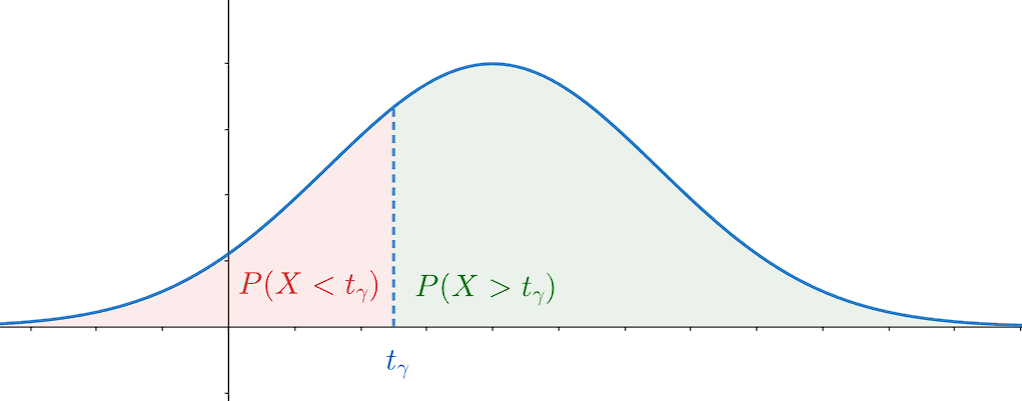
\includegraphics[width=15cm]{mathstat/images/mathstat_2025_03_11_1}
\end{center}

\Ex Медиана - квантиль уровня $\frac{1}{2}$

\DefN{2} Число $t_\alpha$ называется квантилем уровня значимости $\alpha$, если
$P(X > t_\alpha) = \alpha$ или $F(t_\alpha) = 1 - \alpha$

Ясно, что $\gamma = 1 - \alpha$

\subsection{Интервальные оценки}

Недостатки точечных оценок - неизвестно насколько они далеки от реального значения параметра и 
насколько им можно доверять. Особенно это заметно при малых выборках. Поэтому мы указываем интервал, в котором 
лежит этот параметр с заданной вероятностью (надежностью) $\gamma$. Такие оценки называются интервальными 
(доверительными)

\Def Интервал $(\theta^-_\gamma; \theta^+_\gamma)$ называется доверительным интервалом параметра $\theta$
надежности $\gamma$, если вероятность $P(\theta^-_\gamma < \theta < \theta^+_\gamma) = \gamma$

\Nota Если имеем дискретную случайную величину, то $P(\theta^-_\gamma < \theta < \theta^+_\gamma) \geq \gamma$

\Notas Так как параметр $\theta$ - константа, то бесмысленно говорить о его попадании в интервал. Правильно: 
доверительный интервал накрывает параметр $\theta$ с вероятностью $\gamma$

\NotaN{1} $\alpha = 1 - \gamma$ называется уровнем значимости доверительного интервала

\NotaN{2} Обычно пытаются строить симметричный доверительный интервал относительно несмещенной оценки $\theta^*$

\NotaN{3} Возникает вопрос, какой уровень $\gamma$ выбрать для исследования.
Стандартные уровени надежности $\gamma$: $0.9, \ 0.95, \ 0.99, \ 0.999$. Самый мейнстримный - $0.95$. 
В малых выборках используют $0.9$

Вспомним основную теорему:

\begin{MyTheorem}
    $\letsymbol (X_1, \dots, X_n)$ - выборка объема $n$ из $N(\alpha, \sigma^2)$

    $\overline{x}$ - выборочное среднее, $S^2$ - исправленная дисперсия, $D^*$ - выборочная дисперсия

    Тогда:

    \begin{enumerate}
        \item $\sqrt{n} \frac{\overline{x} - a}{\sigma} \in N(0, 1)$
        \item $\sum_{i = 1}^n \left(\frac{X_i - a}{\sigma}\right)^2 = \frac{n \tilde{\sigma^2}}{\sigma^2} \in H_n$, 
        где $n \tilde{\sigma^2} = \sum_{i = 1}^n (X_i - a)^2$
        \item $\sum_{i = 1}^n \left(\frac{X_i - \overline{x}}{\sigma}\right)^2 = \frac{(n - 1)S^2}{\sigma^2} = 
        \frac{nD^*}{\sigma^2} \in H_{n - 1}$
        \item $\sqrt{n} \frac{\overline{x} - a}{S} \in T_{n - 1}$
        \item $\overline{x}$ и $S^2$ - независимы
    \end{enumerate}
\end{MyTheorem}


\Nota Если $F(x)$ - функция симметричного относительно $x = 0$ распределения, то $P(|X| < t) = 2F(t) - 1$

% https://www.geogebra.org/calculator/msnwgfyp

\begin{center}
    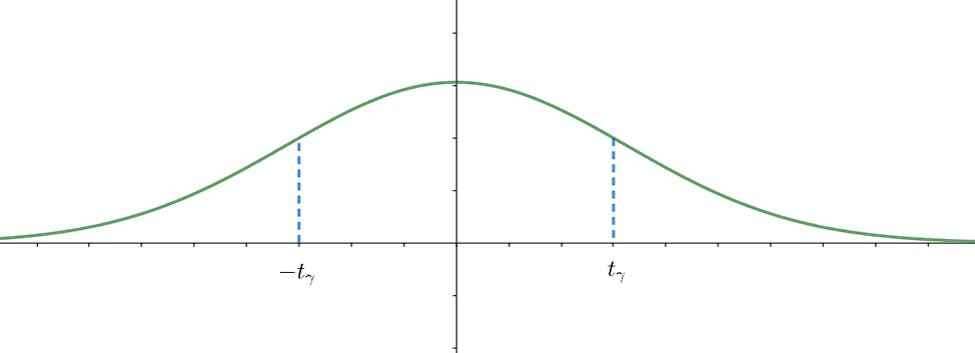
\includegraphics[width=15cm]{mathstat/images/mathstat_2025_03_11_2}
\end{center}

\subsection{Доверительные интервалы для параметров нормального распределения}

Пусть $\vec X = (X_1, \dots, X_n)$ - выборка объема $n$ из $N(a, \sigma^2)$. 
Хотим найти интервалы для параметров $a$ и $\sigma^2$

\begin{enumerate}[label*=\Roman*.]
    \item Доверительный интервал для параметра $a$ при известном значении $\sigma^2$

    По пункту 1 из теоремы $\sqrt{n} \frac{\overline{x} - a}{\sigma} \in N(0, 1)$ 

    $P\left(-t_\gamma < \sqrt{n} \frac{\overline{x} - a}{\sigma} < t_\gamma\right) = 
    P\left(\left|\sqrt{n} \frac{\overline{x} - a}{\sigma}\right| < t_\gamma\right) = 2F_0 (t_\gamma) - 1 = \gamma$

    $F_0(t_\gamma) = \frac{1 + \gamma}{2} \Longrightarrow t_\gamma$ - квантиль уровня 
    $\frac{1 + \gamma}{2}$ для $N(0, 1)$, где
    $F_0(x) = \frac{1}{\sqrt{2\pi}} \int_{-\infty}^{\infty} e^{-\frac{z^2}{2}} dz$

    Решая неравенство, получаем $-t_\gamma < \sqrt{n} \frac{\overline{x} - a}{\sigma} < t_\gamma$

    $-t_\gamma \frac{\sigma}{\sqrt{n}} < \overline{x} - a < t_\gamma \frac{\sigma}{\sqrt{n}}$

    $\overline{x} - t_\gamma \frac{\sigma}{\sqrt{n}} < a < \overline{x} + t_\gamma \frac{\sigma}{\sqrt{n}}$ - 
    симметричный интервал относительно $\overline{x}$

    Доверительный интервал надежности $\gamma$: $\left(\overline{x} - t_\gamma \frac{\sigma}{\sqrt{n}}, 
    \overline{x} + t_\gamma \frac{\sigma}{\sqrt{n}}\right)$, 
    где $t_\gamma$ - квантиль $N(0, 1)$ уровня $\frac{1 + \gamma}{2}$

    \item Доверительный интервал для параметра $a$ при неизвестном $\sigma^2$

    Из пункта 4 из теоремы $\sqrt{n} \frac{\overline{x} - a}{S} \in T_{n - 1}$

    $P\left(-t_\gamma < \sqrt{n} \frac{\overline{x} - a}{S} < t_\gamma\right) = P\left(\left|\sqrt{n} \frac{\overline{x} - a}{S}\right| < t_\gamma\right) = 2F_{T_{n - 1}}(t_\gamma) = \gamma$

    $F_{T_{n - 1}}(t_\gamma) = \frac{1 + \gamma}{2} \Longrightarrow t_\gamma$ - квантиль $T_{n - 1}$ уровня 
    $\frac{1 + \gamma}{2}$

    Аналогично с примером выше получаем интервал $\left(\overline{x} - t_\gamma \frac{S}{\sqrt{n}}, 
    \overline{x} + t_\gamma \frac{S}{\sqrt{n}}\right)$, 
    где $t_\gamma$ - квантиль $T_{n - 1}$ уровня $\frac{1 + \gamma}{2}$

    \item Доверительный интервал для параметра $\sigma^2$ при неизвестном $a$

    По пункту 3 из теоремы $\sum_{i = 1}^n \left(\frac{X_i - \overline{x}}{\sigma}\right)^2 = \frac{(n - 1)S^2}{\sigma^2} = 
    \frac{nD^*}{\sigma^2} \in H_{n - 1}$

    Пусть $\chi_1^2$ и $\chi_2^2$ - квантили $H_{n - 1}$ уровней $\frac{1 - \gamma}{2}$ и $\frac{1 + \gamma}{2}$

    Тогда $P\left(\chi_1^2 < \frac{(n - 1)S^2}{\sigma^2} < \chi_2^2\right) = F_{H_{n - 1}}(\chi_1^2) - F_{H_{n - 1}}(\chi_2^2) = \frac{1 - \gamma}{2} - \frac{1 + \gamma}{2} = \gamma$

    $\chi_1^2 < \frac{(n - 1)S^2}{\sigma^2} < \chi_2^2$

    $\frac{1}{\chi_2^2} < \frac{\sigma^2}{(n - 1)S^2} < \frac{1}{\chi_1^2}$

    $\frac{(n - 1)S^2}{\chi_2^2} < \sigma^2 < \frac{(n - 1)S^2}{\chi_1^2}$ или 
    $\frac{nD^*}{\chi_2^2} < \sigma^2 < \frac{nD^*}{\chi_1^2}$

    Получаем интервал $\left(\frac{(n - 1)S^2}{\chi_2^2}, \frac{(n - 1)S^2}{\chi_1^2}\right)$, где $\chi_1^2$ и $\chi_2^2$ - квантили $H_{n - 1}$ уровней $\frac{1 - \gamma}{2}$ и $\frac{1 + \gamma}{2}$

    \Nota Данный интервал не симметричен относительно неизвестного параметра $\sigma^2$

    \item Доверительный интервал для параметра $\sigma^2$ при известном $a$

    По пункту 2 из теоремы $\sum_{i = 1}^n \left(\frac{X_i - a}{\sigma}\right)^2 = \frac{n \tilde{\sigma^2}}{\sigma^2} \in H_{n - 1}$
    
    Пусть $\chi_1^2$ и $\chi_2^2$ - квантили $H_{n}$ уровней $\frac{1 - \gamma}{2}$ и $\frac{1 + \gamma}{2}$

    Тогда $P\left(\chi_1^2 < \frac{n \tilde{\sigma^2}}{\sigma^2} < \chi_2^2\right) = F_{H_{n}}(\chi_1^2) - F_{H_{n}}(\chi_2^2) = \frac{1 - \gamma}{2} - \frac{1 + \gamma}{2} = \gamma$

    Аналогично получаем интервал $\left(\frac{n \tilde{\sigma^2}}{\chi_2^2}, \frac{n \tilde{\sigma^2}}{\chi_1^2}\right)$, 
    где $\chi_1^2$ и $\chi_2^2$ - квантили $H_{n}$ уровней $\frac{1 - \gamma}{2}$ и $\frac{1 + \gamma}{2}$, $n \tilde{\sigma^2} = \sum_{i = 1}^n (X_i - a)^2$

    \Nota $\tilde{\sigma^2} - D^* = \frac{1}{n} \sum_{i = 1}^n (X_i - a)^2 - \frac{1}{n} \sum_{i = 1}^n (X_i - \overline{x})^2 = 
    \frac{1}{n} \sum_{i = 1}^n (X_i^2 - 2aX_i + a^2 - X_i^2 + 2 \overline{x} X_i - \overline{x}^2) = 
    \frac{1}{n} (na^2 - 2a n \overline{x} + 2 \overline{x} \cdot n \overline{x} - n \overline{x}^2) = 
    a^2 - 2a \overline{x} + \overline{x}^2 = (a - \overline{x})^2 \Longrightarrow \tilde{\sigma^2} = D^* + (a - \overline{x})^2$

    Получаем $\left(\frac{n (D^* + (a - \overline{x})^2)}{\chi_2^2}, \frac{n (D^* + (a - \overline{x})^2)}{\chi_1^2}\right)$

\end{enumerate}

\subsection{Асимптотические доверительные интервалы}

\Def Интервал $(\theta^-_\gamma, \theta^+_\gamma)$ называется асимптотическим доверительным интервалом параметра $\theta$ 
уровня $\gamma$, если $P(\theta^-_\gamma < \theta < \theta^+_\gamma) \underset{n \to \infty}{\longrightarrow} \gamma$

\Ex Доверительный интервал вероятности события $A$

Пусть $p = P(A), q = 1 - p, n$ - число испытаний или объем выборки $(X_1, \dots, X_n)$, где $X_i \in \{0, 1\}$

$p^* = \frac{n_A}{n} = \overline{x}$ - оценка $p$

Согласно Центральной предельной теореме $\sqrt{n} \frac{p^* - p}{D X_1} = \sqrt{n} \frac{p^* - p}{\sqrt{pq}} \rightrightarrows N(0, 1)$

Так как $p^* \overset{p}{\longrightarrow} p$, то $\sqrt{n} \frac{p^* - p}{\sqrt{p^* (1 - p^*)}} = 
\sqrt{n} \underset{\rightrightarrows N(0, 1)}{\underbrace{\frac{p^* - p}{\sqrt{p (1 - p)}}}} \underset{\overset{p}{\longrightarrow} 1}{\underbrace{\frac{\sqrt{p (1 - p)}}{\sqrt{p^* (1 - p^*)}}}} \rightrightarrows N(0, 1)$


$P\left(\left|\sqrt{n} \frac{p^* - p}{\sqrt{p^* (1 - p^*)}}\right| < t_\gamma\right) \underset{n \to \infty}{\longrightarrow} 2F_0(t_\gamma) - 1 = \gamma$

$F_0(t_\gamma) = \frac{1 + \gamma}{2}$, $t_\gamma$ - квантиль $N(0, 1)$ уровня $\frac{1 + \gamma}{2}$

Получаем $\left|\sqrt{n} \frac{p^* - p}{\sqrt{p^* (1 - p^*)}}\right| < t_\gamma$

$|p^* - p| < t_\gamma \frac{\sqrt{p^* (1 - p^*)}}{\sqrt{n}}$

Итак, $\left(-t_\gamma \frac{\sqrt{\overline{x} (1 - \overline{x})}}{\sqrt{n}}, t_\gamma \frac{\sqrt{\overline{x} (1 - \overline{x})}}{\sqrt{n}}\right)$, где $t_\gamma$ - квантиль $N(0, 1)$ уровня $\frac{1 + \gamma}{2}$




% end mathstat_2025_03_11.tex

% begin mathstat_2025_03_18.tex





\section{Лекция 6.}

\subsection{Проверка статистических гипотез}

$\letsymbol \vec X = (X_1, \dots, X_n)$ из некоторого распределения $F$

\Def \underline{Гипотезой} $H$ называется предположение о распределении наблюдаемой случайной величины. 

Доказать какое-то утверждение с помощью методов матстатистики невозможно - можно лишь с какой-то долей 
уверенности утверждать

\Def Гипотеза называется \underline{простой}, если она однозначно определяет распределение: 
$H : F = F_1$, где $F_1$ - распределение известного типа с известными параметрами

В противном случае гипотеза называется \underline{сложной} - она является объединением конечного или бесконечного числа
гипотез

Например, \enquote{величина $X$ принадлежит нормальному распределению} - сложная гипотеза, а 
\enquote{величина $X$ принадлежит нормальному распределению с матожиданием $a = 1$ и дисперсией $\sigma^2 = 1$} - простая


В общем случае работаем со схемой из двух или более гипотез. В ходе проверки принимается ровна одна из них.
Мы ограничемся самой простой схемой из 2 гипотез: $H_0$ - основная (нулевая) гипотеза, $H_1 = \overline{H_0}$ - 
альтернативная (конкурирующая) гипотеза, состоящая в том, что основная гипотеза неверна

Основная гипотеза $H_0$ принимается или отклоняется при помощи \underline{статистики критерия} $K$ 

$K(X_1, \dots, X_n) \longrightarrow \Real = \overline{S} \cup S \longrightarrow (H_0, H_1)$

$\begin{cases}
    H_0, & \text{ если } K(X_1, \dots, X_n) \in \overline{S} \\
    H_1, & \text{ если } K(X_1, \dots, X_n) \in S
\end{cases}$

Вместо \enquote{гипотеза доказана} лучше употреблять \enquote{гипотеза принимается/отвергается}

Область $S$ называется критической областью, а точка $t_\text{кр}$ на границе областей называется критической

\Def \underline{Ошибка первого рода} состоит в том, что $H_0$ отклоняется, хотя она верна. 
Аналогично, ошибка второго рода состоит в том, что $H_1$ отклоняется, хотя она верна.

\Defs \underline{Вероятность $\alpha$ ошибки первого рода} называется уровнем значимости критерия. 
Вероятность ошибки второго рода обозначаем $\beta$. \underline{Мощностью} критерия называется вероятность $1 - \beta$ (вероятность
недопущения ошибки второго рода)

Ясно, что критерий будет тем лучше, чем меньше вероятности ошибок $\alpha$ и $\beta$. При увеличении объема
выборки уменьшаются обе вероятности. При фиксированном объему попытки уменьшить одну вероятность
увеличат другую

Одним из способов является фиксация одной вероятности (принято $\alpha$) и уменьшение другой

\subsection{Построение критериев согласия}

\Def Говорят, что критерий $K$ является критерием асимптотического уровня $\varepsilon$, если 
вероятность ошибки первого рода $\alpha \underset{n \to \infty}{\longrightarrow} \varepsilon$

\Defs Критерий $K$ для проверки гипотезы $H_0$ называется состоятельным, если вероятность ошибки второго рода
$\beta \underset{n \to \infty}{\longrightarrow} 0$

\Defs Критерием согласия уровня $\varepsilon$ называем состоятельный критерий асимптотического уровня
$\varepsilon$

Обычно критерий согласия строится по следующей схеме: берется статистика $K(X_1, \dots, K_n)$, 
обладающая свойствами:

\begin{enumerate}
    \item Если $H_0$ верна, то $K(X_1, \dots, X_n) \rightrightarrows Z$, где $Z$ - известное распределение

    \item Если $H_0$ неверна, то есть верна $H_1$, то $K(X_1, \dots, X_n) \underset{n \to \infty}{\ConvergesInProbability} \infty$ 
    (достаточно сильно отклоняться от распределения $Z$)
\end{enumerate}

\begin{MyTheorem}
    Построенный таким образом критерий является критерием согласия, то есть обладает свойствами

    \begin{enumerate}
        \item критерия асимптотического уровня
        \item состоятельного критерия
    \end{enumerate}
\end{MyTheorem}

\begin{MyProof}
    Пусть $t_\text{кр}$ - критическая точка такая, что $P(|Z| \geq t_\text{кр}) = \varepsilon$ - заданный уровень ошибки первого рода

    \begin{cases}
        H_0, & \text{ если } |K| < t_\text{кр} \\ 
        H_1, & \text{ если } |K| \geq t_\text{кр} \\ 
    \end{cases}

    \begin{enumerate}
        \item Тогда $\alpha = P(|K| \geq t_\text{кр} \ | \ H_0) = 1 - P(|K| < t_\text{кр} \ | \ H_0) = 1 - (F_K(t_\text{кр}) - F_K(-t_\text{кр})) 
        \overset{\substack{\text{т.к. при верной } H_0 \\ F_K(x) \underset{n \to \infty}{\longrightarrow} F_Z(x)}}{\underset{n \to \infty}{\relbar\joinrel\relbar\joinrel\longrightarrow}} 
        1 - (F_Z(t_\text{кр}) - F_Z(-t_\text{кр})) = P(|Z| \geq t_\text{кр}) = \varepsilon$

        \item Если $H_1$ верна, то $|K| \ConvergesInProbability \infty$, то есть $\forall C \ P(|K| > C \ | \ H_1) \ConvergesInProbability 1 \Longrightarrow 
        \beta = P(|K| < C \ | \ H_1) \ConvergesInProbability 0$
    \end{enumerate}
\end{MyProof}

\subsection{Гипотеза о среднем нормальной совокупности при известной дисперсии}

$\letsymbol \vec X = (X_1, \dots, X_n)$ из $N(a, \sigma^2)$, причем $\sigma^2$ известен.

Проверяется гипотеза, что $H_0 \, : \, a = a_0$, против $H_1 \, : \, a \neq a_0$ для уровня значимости $\alpha$

\begin{enumerate}
    \item По пункту 1 теоремы, если $H_0 \, : \, a = a_0$ верна, то $K = \sqrt{n} \frac{\overline{x} - a_0}{\sigma} = 
    \sqrt{n} \frac{\overline{x} - a}{\sigma} \in N(0, 1)$
    
    \item Если верна $H_1 \, : a \neq a_0$, то $|K| = \sqrt{n} \left|\frac{\overline{x} - a_0}{\sigma}\right| = 
    \sqrt{n} \left|\frac{\overline{x} - a}{\sigma} + \frac{a - a_0}{\sigma}\right| = \\
     = \left|\underset{\substack{\in N(0, 1), \text{ограничен}\\ \text{по вероятности}}}{\underbrace{\sqrt{n} \frac{\overline{x} - a}{\sigma}}} + \underset{\to \infty}{\underbrace{\sqrt{n}}} \underset{\operatorname{const}}{\underbrace{\frac{a - a_0}{\sigma}}}\right|
    \ConvergesInProbability \infty$
\end{enumerate}

Для уровня значимости $\alpha$ находим $t_\text{кр}$ такую,
что $\alpha = P(|K| \geq t_\text{кр} \ | \ H_0)=  P(|Z| \geq t_\text{кр}) \Longrightarrow P(|Z| < t_\text{кр}) = 2F_0(t_\text{кр}) - 1 = 1 - \alpha$

$F_0(t_\text{кр}) = 1 - \frac{\alpha}{2}$ - то есть $t_\text{кр}$ - квантиль стандартного нормального распределения уровня $1 - \frac{\alpha}{2}$

\begin{cases}
    H_0, & \text{ если } |K| < t_\text{кр} \\ 
    H_1, & \text{ если } |K| \geq t_\text{кр} \\ 
\end{cases}

\subsection{Гипотеза о среднем нормальной совокупности при неизвестной дисперсии}

\begin{enumerate}
    \item По пункту 4 основной теоремы, если $H_0 \, : \, a = a_0$ верна, то $K = \sqrt{n} \frac{\overline{x} - a_0}{S} = 
    \sqrt{n} \frac{\overline{x} - a}{S} \in T_{n - 1}$
    
    \item Если верна $H_1 \, : a \neq a_0$, то $|K| = \sqrt{n} \left|\frac{\overline{x} - a_0}{S}\right| = 
    \sqrt{n} \left|\frac{\overline{x} - a}{S} + \frac{a - a_0}{S}\right| = \\
     = \left|\underset{\substack{\in T_{n - 1}, \text{ограничен}\\ \text{по вероятности}}}{\underbrace{\sqrt{n} \frac{\overline{x} - a}{S}}} + \underset{\to \infty}{\underbrace{\sqrt{n}}} \underset{\operatorname{const}}{\underbrace{\frac{a - a_0}{S}}}\right|
    \ConvergesInProbability \infty$
\end{enumerate}

Аналогично получаем $t_\text{кр}$ - квантиль распределения $T_{n - 1}$ уровня $1 - \frac{\alpha}{2}$

\subsection{Доверительные интервалы как критерии гипотез по параматрам распределения}

$\letsymbol (X_1, \dots, X_n)$ из $F_\theta$, где $F_\theta$ - распределение известного типа с неизвестным параметром $\theta$

Проверяется гипотеза, что $H_0 \, : \, \theta = \theta_0$, против $H_1 \, : \, \theta \neq \theta_0$

Допустим, что для $\theta$ построен доверительный интервал $(\theta_\gamma^-, \theta_\gamma^+)$, то есть 
$P(\theta_\gamma^- < \theta < \theta_\gamma^+) = \gamma$.

Тогда критерий 
\begin{cases}
    H_0, & \text{ если } \theta_0 \in (\theta_\gamma^-, \theta_\gamma^+) \\ 
    H_1, & \text{ если } \theta_0 \not\in (\theta_\gamma^-, \theta_\gamma^+) \\ 
\end{cases} будет уровня $\alpha = 1 - \gamma$

$\alpha = P(\theta_0 \not\in (\theta_\gamma^-, \theta_\gamma^+) \ | \ H_0) = 1 - P(\theta_0 \in (\theta_\gamma^-, \theta_\gamma^+) \ | \ X \in F_{\theta_0}) = 1 - \gamma$

Поэтому доверительные интервалы можно использовать для проверки гипотез

\mediumvspace 

Но почему в схеме \begin{cases}
    H_0 \, : \, a = \overline{x} \\
    H_1 \, : \, a \neq \overline{x} \\
\end{cases} основная гипотеза всегда верна, тогда как выборочно среднее на практике почти всегда не равняется матожиданию. Потому что ...

\begin{tcolorbox}
    А вот нефиг такие гипотезы вообще выдвигать

    \hfill ©️ Блаженов А. В.
\end{tcolorbox}

\subsection{Критерий вероятности появления события}

$\letsymbol P(A) = p$ - вероятность успеха при одном испытании. При достаточно большом количестве испытаний $n$ событие $A$ появилось $m$ раз.
Проверяется $H_0: \, p = p_0$ против $H_1: \, p \neq p_0$

В качестве статистики критерия возьмем величину $K = \frac{m - np_0}{\sqrt{np_0 q_0}}$

\begin{enumerate}
    \item Если $H_0$ верна, то $K = \frac{m - np}{\sqrt{npq}} \rightrightarrows N(0, 1)$ по ЦПТ

    \item \Lab
\end{enumerate}

Из тех же соображений $t_\text{кр}$ - квантиль $N(0, 1)$ уровня $1 - \frac{\alpha}{2}$

\begin{cases}
    H_0: \, p = p_0, & \text{ если } |K| < t_\text{кр} \\
    H_1: \, p \neq p_0  & \text{ если } |K| \geq t_\text{кр} \\
\end{cases}

\Ex При посеве 4000 семян 970 всходов оказались рецессивного цвета, а 3030 - доминантного. 
Проверим гипотезу $H_0: p = \frac{1}{4}$ - Мендель прав, против $H_1: p \neq \frac{1}{4}$ - Мендель не прав, для уровня значимости - $0.05$

$K = \frac{m - np_0}{\sqrt{np_0 q_0}} = \frac{970 - 4000 \cdot \frac{1}{4}}{\sqrt{4000 \frac{1}{4} \frac{3}{4}}} \approx -1.095$

Так как $|K| = 1.095 < 1.96 = t_\text{кр}$, то $H_0: \, p = \frac{1}{4}$ верна

% end mathstat_2025_03_18.tex

% begin mathstat_2025_03_25.tex





\section{Лекция 7.}

\subsection{Критерии для проверки гипотез о распределении}

\subsubsection{Простая параметрическая гипотеза}

Пусть имеется выборка $(X_1, \dots, X_n)$ объема $n$ из неизвестного распределения $\mathcal{F}$. 
Проверяется простая гипотеза $H_0 : \mathcal{F} = \mathcal{F}_1$ против $H_1 : \mathcal{F} \neq \mathcal{F}_1$, где $\mathcal{F}_1$ - распределение известного типа с 
известными нами параметрами $\theta = (\theta_1, \dots, \theta_m)$

\begin{enumerate}[label*=\Roman*. ]
    \item \textbf{Критерий Колмогорова}

    Если $\mathcal{F}_1$ - \underline{абсолютно непрерывное} распределение с функцией распределения $F(x)$, то применим критерий

    $\letsymbol K = \sqrt{n} \sup_x |F^*(x) - F(x)|$, где $F^*(x)$ - выборочная функция распределения

    То есть используем теорему Колмогорова: если $H_0 : \mathcal{F} = \mathcal{F}_1$, то $K =\sqrt{n} \sup_x |F^*(x) - F(x)| 
    \rightrightarrows \mathcal{K}$ - распределение Колмогорова 
    с функцией распределения $F_\mathcal{K}(x) = \sum_{j = -\infty}^\infty (-1)^j e^{-2j^2 x^2}$

    Для уровня значимости $\alpha$ находим квантиль $t_\alpha$ такой, что $P(\xi \geq t_\alpha) = \alpha$, 
    где $\xi \in \mathcal{K}$

    \begin{cases}
        H_0 : \mathcal{F} = \mathcal{F}_1, & \text{если } K < t_\alpha \\
        H_1 : \mathcal{F} \neq \mathcal{F}_1, & \text{если } K \geq t_\alpha \\
    \end{cases}

    \item \textbf{Критерий \enquote{хи-квадрат} Пирсона}

    Пусть выборка разбита на $k$ интервалов $A_1, A_2, \dots, A_k$, $A_i = [a_{i - 1}, a_1)$

    $n_i$ - соответствующая частота интервала

    При распределении $\mathcal{F}_1$ теоретические вероятности попадания в эти интервалы $p_i = F_{\mathcal{F}_1}(a_i) - F_{\mathcal{F}_1}(a_{i - 1})$.
    Тогда $n_i^\prime = p_i \cdot n$ - теоретические частоты


    В качестве статистики критерия выберем $\chi^2_\text{набл.} = \sum_{i = 1}^k \frac{(n_i - n_i^\prime)^2}{n_i^\prime}$

    \begin{MyTheorem}
        \ThNs{Пирсона} Если $H_0 : \mathcal{F} = \mathcal{F}_1$ верна, то $\chi^2_\text{набл.} \rightrightarrows \chi^2_{k - 1}$ - 
        распределение \enquote{хи-квадрат} с $k - 1$ степенями свободы
    \end{MyTheorem}

    Критерий: $\letsymbol t_\alpha$ - квантиль $\chi^2_{k - 1}$ уровня $\alpha$

    \begin{cases}
        H_0 : \mathcal{F} = \mathcal{F}_1, & \text{если } \chi^2_\text{набл.} < t_\alpha \\
        H_1 : \mathcal{F} \neq \mathcal{F}_1, & \text{если } \chi^2_\text{набл.} \geq t_\alpha \\
    \end{cases}

    \Nota Часто обозначают $t_\alpha = \chi^2_\text{теор.}$

    \Notas При этом частота каждого интервала должна быть не меньше 5, а объем выборки - не меньше 50. 
    Число интервалов лучше брать по формуле Стерджесса
\end{enumerate}

\subsubsection{Сложная параметрическая гипотеза}

Здесь мы будем проверять гипотезу $H_0 : \mathcal{F} \in \mathcal{F}_\theta$ против $H_1 : \mathcal{F} \not\in \mathcal{F}_\theta$, где $\mathcal{F}_\theta$ - распределение 
известного типа с неизвестными параметрами

\begin{enumerate}[label*=\Roman*. ]
    \setcounter{enumi}{2}

    \item \textbf{Критерий \enquote{хи-квадрат} Фишера}

    Пусть выборка разбита на $k$ интервалов $A_1, A_2, \dots, A_k$, $A_i = [a_{i - 1}, a_1)$

    $n_i$ - соответствующая частота интервала $A_i$

    \Def Оценка максимального правдоподобия по частотам называется значения неизвестных параметров,
    при которых вероятность появления таких частот явялется максимальной

    Пусть $\hat \theta = (\hat \theta_1, \dots, \hat \theta_n)$ - оценка максимального правдоподобия 
    по частотам неизвестных параметров. Тогда теоретические вероятности попадания в интервал считаем по формуле 
    $p_i = F_{\mathcal{F}_\theta} (a_i) - F_{\mathcal{F}_\theta} (a_{i - 1})$, теоретическая частота - $n_i^\prime = n p_i$

    В качестве статистики критерия берется функция $\chi^2_\text{набл.} = \sum_{i = 1}^k \frac{(n_i - n_i^\prime)^2}{n_i^\prime}$

    \begin{MyTheorem}
        \ThNs{Фишера} 
        
        Если $H_0 : \mathcal{F} \in \mathcal{F}_\theta$ верна, 
        то $\chi^2_\text{набл.} = \sum_{i = 1}^k \frac{(n_i - n_i^\prime)^2}{n_i^\prime} \rightrightarrows \chi^2_{k - m - 1}$ - 
        распределение \enquote{хи-квадрат}, где $m$ - число параметров неизвестного распределения
    \end{MyTheorem}
    
    $\letsymbol t_\alpha$ - квантиль $\chi^2_{k - m - 1}$ уровня $\alpha$

    \begin{cases}
        H_0 : \mathcal{F} = \mathcal{F}_1, & \text{если } \chi^2_\text{набл.} < t_\alpha \\
        H_1 : \mathcal{F} \neq \mathcal{F}_1, & \text{если } \chi^2_\text{набл.} \geq t_\alpha \\
    \end{cases}

    \Nota Часто в качестве оценки неизвестных параметров берется просто оценка максимального правдоподобия
    
\end{enumerate}

\Ex Имеется выборка в виде вариационного ряда $(5.2; \dots; 22.8)$, $n = 120$, при разбиении на $k = 8$ интервалов получили

\begin{tabular}{c|c|c|c|c|c|c|c|c|c}
    $A_i$ & $[5.2, 7.4)$ & $[7.4, 9.6)$ & $[9.6, 11.8)$ & $[11.8, 14)$ & $[14, 16.2)$ & $[16.2, 18.4)$ & $[18.4, 20.6)$ & $[20.6, 22.8)$ & $\sum$ \\
    \hline
    $n_i$ & 12 & 17 & 14 & 13 & 18 & 14 & 13 & 19 & 120
\end{tabular}

Проверить гипотезу о равномерном распределении $H_0 : \mathcal{F} \in U(a, b)$ против $H_1 : \mathcal{F} \not\in U(a, b)$ при уровне значимости $\alpha = 0.05$

Дадим оценку параметров методом максимального правдоподобия: $\hat a = 5.2 \quad \hat b = 22.8$

Теоретическая вероятность будет $p_i^\prime = \frac{1}{8}$, теоретическая частота - $n_i = 15$

$\chi^2_\text{набл.} = \sum_{i = 1}^k \frac{(n_i - n_i^\prime)^2}{n_i^\prime} = \frac{(12 - 15)^2}{15} + 
\frac{(17 - 15)^2}{15} + \frac{(14 - 15)^2}{15} + \frac{(13 - 15)^2}{15} + \frac{(18 - 15)^2}{15} + 
\frac{(14 - 15)^2}{15} + \frac{(19 - 15)^2}{15} = 3.2$

При $\alpha = 0.05$ и $S = k - m - 1 = 5$ квантиль $\chi^2_S$ уровня $\alpha$ равен $t_\alpha = 11.07$

Так как $\chi^2_\text{набл.} < t_\alpha$, нулевая гипотеза о равномерном распределении принимается

\subsection{Критерии для проверки однородности}

\begin{enumerate}[label*=\Roman*. ]
    \setcounter{enumi}{3}

    \item \textbf{Критерий Колмогорова-Смирнова}

    Пусть имеются 2 независимых выборки $(X_1, \dots, X_n)$ и $(Y_1, \dots, Y_m)$ объемов $n$ и $m$ из неизвестных непрерывных распределений $\mathcal{F}$ и $\mathcal{J}$

    Проверяется $H_0 : \mathcal{F} = \mathcal{J}$ (данные однородны) против $H_1 : \mathcal{F} \neq \mathcal{J}$

    В качестве статистики критерия берется функция $K = \sqrt{\frac{nm}{n + m}} \sup_x |F^*(x) - G^*(x)|$, где $F^*$ и $G^*$ - 
    соответствующие выборочные функции распределения

    \begin{MyTheorem}
        \ThNs{Колмогорова-Смирнова}

        Если $H_0 : \mathcal{F} = \mathcal{J}$ верна, то $K \rightrightarrows \mathcal{K}$ - распределение Колмогорова
    \end{MyTheorem}

    Критерий: $t_\alpha$ - квантиль $\mathcal{K}$ уровня значимости $\alpha$

    \begin{cases}
        H_0 : \mathcal{F} = \mathcal{J}, & \text{если } K < t_\alpha \\
        H_1 : \mathcal{F} \neq \mathcal{J}, & \text{если } K \geq t_\alpha \\
    \end{cases}

\end{enumerate}

\subsubsection{Проверки однородности выборок из нормальных совокупностей}


\begin{enumerate}[label*=\Roman*. ]
    \setcounter{enumi}{4}

    \item \textbf{Критерий Фишера}

    Пусть имеют две независимые выборки $(X_1, \dots, X_n)$ и $(Y_1, \dots, Y_m)$ объемов $n$ и $m$ из нормальных распределений $X \in N(a_1, \sigma^2_1)$ и $Y \in N(a_2, \sigma^2_2)$

    Проверяется $H_0 : \sigma_1 = \sigma_2$ против $H_1 : \sigma_1 \neq \sigma_2$

    В качестве статистики критерия берется функция $K = \frac{S_X^2}{S_Y^2}$, где $S_X^2$, $S_Y^2$ - соответствующие исправленные дисперсии, причем
    $S_X^2 \geq S_Y^2$

    \begin{MyTheorem}
        \Ths Если $H_0 : \sigma_1 = \sigma_2$ верна, то $K = \frac{S_X^2}{S_Y^2} \in F(n - 1, m - 1)$ - распределение Фишера-Снедекера
    \end{MyTheorem}

    \begin{MyProof}
        По пункту 3 основной теоремы $\frac{(n - 1)S^2}{\sigma^2} \in \chi^2_{n - 1}$. Если $H_0$ верна, то $K = \frac{S_X^2}{S_Y^2} = \frac{(n - 1) S_X^2 \sigma_2^2}{\sigma_1^2 (m - 1) S_Y^2} \frac{(m - 1)}{(n - 1)} = \frac{\frac{\chi^2_{n - 1}}{n - 1}}{\frac{\chi^2_{m - 1}}{m - 1}} \in F(n - 1, m - 1)$
    \end{MyProof}

    $t_\alpha$ - квантиль $F(n - 1, m - 1)$ уровня $\alpha$

    \begin{cases}
        H_0 : \sigma_1 = \sigma_2, & \text{если } K < t_\alpha \\
        H_1 : \sigma_1 \neq \sigma_2, & \text{если } K \geq t_\alpha \\
    \end{cases}

    \Nota Здесь критерий согласия работает чуть иным образом: при верной альтернативной гипотезе $K = \frac{S_X^2}{S_Y^2} \ConvergesInProbability \frac{\sigma_1^2}{\sigma_2^2} > 1$

    Если нулевая гипотеза отклоняется, то отклоняется общая гипотеза об однородности. А если основная гипотеза принимается, то 
    применяем критерий Стьюдента

    \item \textbf{Критерий Стьюдента}

    Пусть $(X_1, \dots, X_n)$ и $(Y_1, \dots, Y_m)$ из нормальных распределений $X \in N(a_1, \sigma^2)$ и $Y \in N(a_2, \sigma^2)$

    Проверяется $H_0 : a_1 = a_2$ против $H_1 : a_1 \neq a_2$

    \begin{MyTheorem}
        \Ths $\sqrt{\frac{nm}{n + m}} \frac{(\overline x - a_1) - (\overline y - a_2)}{\sqrt{\frac{(n - 1) S_X^2 + (m - 1) S^2_Y}{n + m - 2}}} \in T_{n + m - 2}$
    \end{MyTheorem}

    \begin{MyProof}
        По пункту 5 основной теоремы считаем, что числитель и знаменатель независимы 

        $\sqrt{\frac{nm}{n + m}} \frac{(\overline x - a_1) - (\overline y - a_2)}{\sqrt{\frac{(n - 1) S_X^2 + (m - 1) S^2_Y}{n + m - 2}}} = 
        \sqrt{\frac{nm}{n + m}} \frac{\frac{\overline x - a_1}{\sigma} - \frac{\overline y - a_2}{\sigma}}{\sqrt{\frac{(n - 1) S_X^2 + (m - 1) S^2_Y}{\sigma^2 (n + m - 2)}}}$

        По пункту 1 основной теоремы $\sqrt{n} \frac{\overline x - a_1}{\sigma}, \sqrt{m} \frac{\overline y - a_2}{\sigma} \in N(0, 1) \Longrightarrow \\
        \frac{\overline x - a_1}{\sigma} \in N\left(0, \frac{1}{n}\right), \frac{\overline y - a_2}{\sigma} \in N\left(0, \frac{1}{m}\right) \Longrightarrow \\
        \frac{\overline x - a_1}{\sigma} - \frac{\overline y - a_2}{\sigma} \in N\left(0, \sqrt{\frac{n + m}{nm}}\right) \Longrightarrow \\
        \sqrt{\frac{nm}{n + m}} \left(\frac{\overline x - a_1}{\sigma} - \frac{\overline y - a_2}{\sigma}\right) \in N(0, 1)$

        По пункту 3 основной теоремы $\frac{(n - 1)S^2_X}{\sigma^2} \in \chi^2_{n - 1}, \frac{(m - 1)S^2_Y}{\sigma^2} \in \chi^2_{m - 1} \Longrightarrow
        \frac{(n - 1) S_X^2 + (m - 1) S^2_Y}{\sigma^2 (n + m - 2)} \in \frac{\chi^2_{n + m - 2}}{m + n - 2}$

        Из этого $\sqrt{\frac{nm}{n + m}} \frac{(\overline x - a_1) - (\overline y - a_2)}{\sqrt{\frac{(n - 1) S_X^2 + (m - 1) S^2_Y}{n + m - 2}}} \in \frac{N(0, 1)}{\frac{\chi^2_{n + m - 2}}{n + m - 2}} = T_{n + m - 2}$
    \end{MyProof}

    В качестве статистики возьмем $\sqrt{\frac{nm}{n + m}} \frac{(\overline x - a_1) - (\overline y - a_2)}{\sqrt{\frac{(n - 1) S_X^2 + (m - 1) S^2_Y}{n + m - 2}}}$, 
    по теореме при $a_1 = a_2$ получаем, что $K \in T_{n + m - 2}$

    Если верна альтернативная гипотеза, то $K \longrightarrow \infty$

    Критерий: $t_\alpha$ - квантиль $|T_{n + m - 2}|$ уровня $\alpha$

    \begin{cases}
        H_0 : a_1 = a_2, & \text{если } K < t_\alpha \\
        H_1 : a_1 \neq a_2, & \text{если } K \geq t_\alpha \\
    \end{cases}

    \Nota Если при обоих критериях согласились с нулевой гипотезой, то соглашаемся с гипотезой об однородности выборок

    \Notas Критерий хорошо работает, если выборки из нормальных распределении (или очень близких к ним)

\end{enumerate}


% end mathstat_2025_03_25.tex

% begin mathstat_2025_04_01.tex





\section{Лекция 8.}

\subsection{Статистическая зависимость}

\Def Зависимость называется статистической, если изменение одной случайной величины вызывает 
изменение распределения другой.
Если при этом изменяется среднее значение другой случайной величины, то такая зависимость называется коррелеционной. 
Если при увеличении одной случайной величины среднее значение другой также увеличивается, то говорят, 
что имеет место прямая корреляция. Аналогично, если уменьшается, то -- обратная

\subsection{Корреляционное облако}

Пусть в ходе $n$ экспериментов появились значения двух случайных величин $X$ и $Y$: 

$(x_1, y_1), (x_2, y_2), \dots, (x_n, y_n)$

Нанеся точки на координатную плоскость, получаем корреляционное облако, о виде которого можно делать предположения о наличии/отсутствии связи

% https://www.geogebra.org/calculator/vjhcvrjr

\Ex 

\begin{multicols}{2}
    \begin{center}
        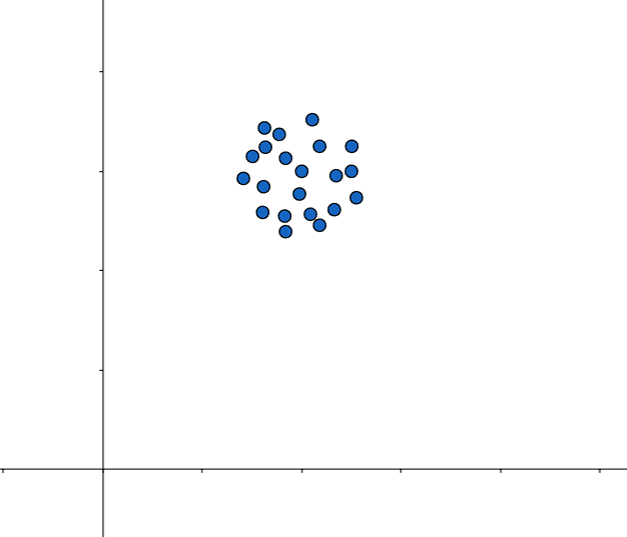
\includegraphics[height=5cm]{mathstat/images/mathstat_2025_04_01_1}

        Здесь, возможно, нет зависимости

        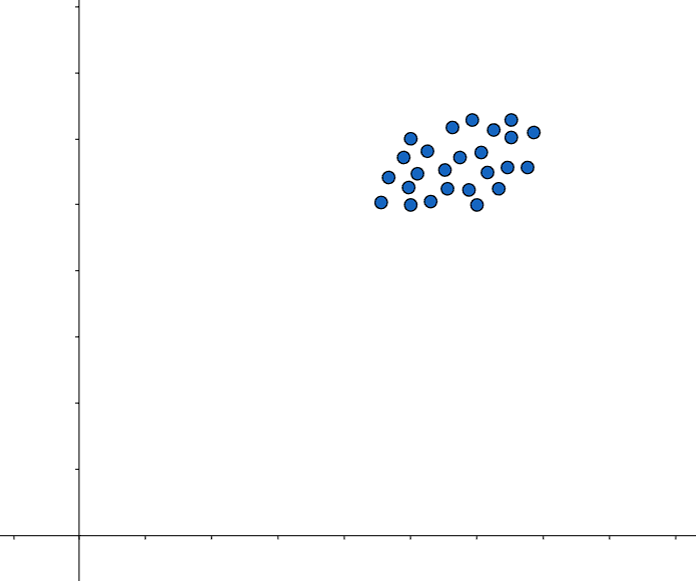
\includegraphics[height=5cm]{mathstat/images/mathstat_2025_04_01_2}

        Здесь можно предположить прямую корреляцию
    \end{center}
\end{multicols}

\subsection{Корреляционная таблица}

Пусть даны данные $X$ и $Y$ при $n$ экспериментов. Эти данные удобно представить в виде коррелеционной таблицы:
по вертикали отмечают различные значения $x$, а по горизонтали - $y$, в клетках таблицы отмечаются частота появления $n_{xy}$

\Ex $n = 50$

\smallvspace

\begin{tabular}{c|c|c|c|c|c|c}
    X\backslash Y & 10 & 20 & 30 & 40 & $n_x$ & $\overline y_x$ \\
    \hline
    2 & 7 & 3 & 0 & 0 & 10 & 13 \\
    \hline
    4 & 3 & 10 & 10 & 2 & 25 & 4.4 \\
    \hline
    6 & 0 & 2 & 10 & 3 & 15 & 30.67 \\
    \hline
    $n_y$ & 10 & 15 & 20 & 5 & $\Sigma$ 50 & \\
\end{tabular}

\smallvspace

По диагонали таблицы можно предположить, что корреляция есть

Имеет смысл вычислить условное среднее по формуле $\overline y (x) = \frac{1}{n_x} \sum n_{xy} y_i$. Так как в нашем примере
условные средние растут с ростом $x$, то имеет место прямая корреляция

\Nota Если данных много или $X$ и $Y$ -- непрерывные случайные величины, то лучше составить интервальную корреляционную таблицу:
разбить случайные величины на интервалы, по вертикали отметить интервалы $[a_{i - 1}, a_i)$ случайной величины $X$, 
по горизонтали -- $[b_{j - 1}, b_j)$ случайной величины $Y$, в клетках 
отметить частоты $n_{ij} : [a_{i - 1}, a_i) \times [b_{j - 1}, b_j)$. В дальнейшем интервалы можно заменить их серединами

\subsection{Критерий \enquote{хи-квадрат} для проверки независимости}

Пусть выборка $(X_1, Y_1), (X_2, Y_2), \dots, (X_n, Y_n)$ представлена в виде интервальной корреляционной таблицы. Случайная величина $X$ 
разбита на $k$ интервалов, а $Y$ -- на $m$ интервалов

Обозначим $v_{i\cdot}$ -- частота $i$-ого интервала $[a_{i - 1}, a_i)$ случайной величины $X$, 
$v_{\cdot j}$ -- частота $j$-ого интервала $[b_{j - 1}, b_j)$ случайной величины $Y$, $v_{ij}$ -- число точек в $[a_{i - 1}, a_i) \times [b_{j - 1}, b_j)$


\begin{tabular}{c|c|c|c|c|c}
    X\backslash Y & $[b_0, b_1)$ & $[b_1, b_2)$ & \dots & $[b_{m - 1}, b_m)$ & $v_{i\cdot}$ \\
    \hline
    $[a_0, a_1)$ & $v_{11}$ & $v_{12}$ & \dots & $v_{1m}$ & $v_{1\cdot}$ \\
    \hline
    \multicolumn{6}{c}{\dots} \\
    \hline
    $[a_{k - 1}, a_k)$ & $v_{k1}$ & $v_{k2}$ & \dots & $v_{km}$ & $v_{k\cdot}$ \\
    \hline
    $v_{\cdot j}$ & 10 & 15 & 20 & 5 & $\Sigma n$ \\
\end{tabular}

Проверяется основная гипотеза $H_0 : X \text{ и } Y$ независимы против $H_1 = \overline{H_0} : X \text{ и } Y$ зависимы

Если $H_0$ верна, то $p_{ij} = P(X \in [a_{i - 1}, a_i), Y \in [b_{j - 1}, b_j)) = P(X \in [a_{i - 1}, a_i)) \cdot P(Y \in [b_{j - 1}, b_j))$

Тогда по закону больших чисел $\frac{v_{i\cdot}}{n} \ConvergesInProbability p_{i\cdot}, \frac{v_{\cdot j}}{n} \ConvergesInProbability p_{\cdot j}$

Поэтому основанием для отклонения основной гипотезы будет заметная разница между величинами $\frac{v_{i\cdot}}{n}\frac{v_{\cdot j}}{n}$ и 
$\frac{v_{ij}}{n}$ или $v_{ij}$ и $\frac{1}{n} v_{i\cdot} v_{\cdot j}$

В качестве статистики берется $K = n \sum_{i, j} \frac{\left(v_{ij} - \frac{1}{n} v_{i\cdot} v_{\cdot j}\right)^2}{v_{i\cdot} v_{\cdot j}}$

\begin{MyTheorem}
    \Ths Если $H_0$ верна, то $K \rightrightarrows H_{(k - 1)(m - 1)}$
\end{MyTheorem}

Пусть $t_\alpha$ -- квантиль $H_{(k - 1)(m - 1)}$ уровня $\alpha$, тогда 

\begin{cases}
    H_0 : X \text{ и } Y \text{ независимы, если } K < t_\alpha \\
    H_0 : X \text{ и } Y \text{ зависимы, если } K \geq t_\alpha \\
\end{cases}

\Nota Для работы критерия необходимо, что бы частота в каждой клетке была больше 5, а объем выборки был достаточно большой

\subsection{Однофакторный дисперсионный анализ}

Предположим, что на случайную величину $X$ (результат) может влиять фактор $Z$ (необязательно, что $Z$ -- случайная величина, эксперимент может быть управляемым)

Пусть при различных \enquote{$k$ уровней} фактора $Z$ получено $k$ независимых выборок случайной величины $X$: 
$X^{(1)} = (X_1^{(1)}, \dots, X^{(1)}_{n_1}), \dots, X^{(k)} = (X_1^{(k)}, \dots, X^{(k)}_{n_k})$

Всего было получено $n = \sum_{i = 1}^k n_i$ значений

\Nota В общем говоря, распределение этих выборок отличается, поэтому эти выборки разных случайных величин

\subsubsection{Общая, внутригрупповая и межгрупповая дисперсии}

Для каждой выборки вычислим выборочное среднее и дисперсию: $\overline{x}^{(j)} = \frac{1}{n_j} \sum_{i = 1}^{n_j} X_i^{(j)}$, 
$D^{(j)} = \frac{1}{n_j} \sum_{i = 1}^{n_j} (X_i^{(j)} - \overline{x}^{(j)})^2$

Объединим все выборки в общую и также вычислим выборочнее среднее и дисперсию: 

$\overline{x} = \frac{1}{n} \sum_{i, j} x^{(j)}_i = \frac{1}{n} \sum_{j = 1}^k n_j \cdot \overline{x}^{(j)}$ - общее среднее

$D_\text{О} = \frac{1}{n} \sum_{i, j} (X^{(j)}_i - \overline{x})^2$ - общая дисперсия

\Def Внутригрупповой (или остаточной) дисперсией называется среднее групповых дисперсий: $D_{\text{В}} = \frac{1}{n} \sum_{j = 1}^k n_j D^{(j)}$

\Def Межгрупповой (или факторной) дисперсией называется величина $D_{\text{М}} = \frac{1}{n} \sum_{j = 1}^k n_j (\overline{x} - \overline{x}^{(j)})^2$

\begin{MyTheorem}
    \ThNs{О разложении дисперсии} Общая дисперсия равна сумме внутригрупповой и межгрупповой дисперсией: $D_\text{О} = D_\text{В} + D_\text{М}$
\end{MyTheorem}

Смысл: внутригрупповая дисперсия показывает средний (случайный) разброс внутри выборок, межгрупповая - насколько отличаются среднее при различных 
уровнях фактора, то есть именно эта величина отражает влияния фактора

Вывод по наличии корреляции можно сделать, если доля $D_\text{М}$ достаточно велика

\subsubsection{Проверка гипотезы о влиянии фактора}

Предполагаем, что $X$ имеет нормальное распределение и фактор $Z$ может влиять только на ее математическое ожидание, 
но не на дисперсию и тип распределения, поэтому можно считать, что данные независимых $k$ выборок при различных уровнях фактора $Z$
также имеют нормальное распределение с одинаковой дисперсией: $X^{(j)} \in N(a_j, \sigma^2)$

Проверяется основная гипотеза $H_0 : a_1 = a_2 = \dots = a_k$ (фактор не оказывает влияния) против $H_1 = \overline{H_0} : $ есть влияние

По пункту 3 основной теоремы $\sum_{i = 1}^n \left(\frac{x_i - \overline{x}}{\sigma}\right)^2 = \frac{n D^*}{\sigma^2} \in H_{n - 1}$

Из этого $\frac{n_j D^{(j)}}{\sigma^2} \in H_{n_j - 1} \quad \forall \ 1 \leq j \leq k$

Так как распределение \enquote{хи-квадрат} устойчиво относительно суммирования, то $\sum_{j = 1}^k \frac{n_j D^{(j)}}{\sigma^2} \in H_{n - k}$, так как
$(n_1 - 1) + \dots + (n_k - 1) = n - k$

Пусть основная гипотеза верна, тогда все данные можно считать выборкой одной случайной величины и по пункту 3 $\frac{n D_{\text{О}}}{\sigma^2} \in H_{n - 1}$

Согласно теореме о разложении дисперсии $D_\text{О} = D_\text{В} + D_\text{М}$, тогда $\frac{n D_{\text{О}}}{\sigma^2} = \frac{n D_{\text{В}}}{\sigma^2} + \frac{n D_{\text{М}}}{\sigma^2}$

Так как $\frac{n D_{\text{О}}}{\sigma^2} \in H_{n - 1}, \frac{n D_{\text{В}}}{\sigma^2} \in H_{n - k}$, то $\frac{n D_{\text{М}}}{\sigma^2} \in H_{k - 1}$

Тогда при верной основной гипотезе получим, что $\frac{n D_{\text{М}}}{\sigma^2} \frac{\sigma^2 (n - k)}{n D_\text{В}} = \frac{n - k}{k - 1} \frac{D_\text{М}}{D_\text{В}} \in F(k - 1, n - k)$ --
распределение Фишера-Снедекера со степенями $k - 1$ и $n - k$

В качестве статистики берется $K = \frac{n - k}{k - 1} \frac{D_\text{М}}{D_\text{В}}$, в качестве критической точки $t_\alpha$ -- квантиль $F(k - 1, n - k)$ уровня $\alpha$

\begin{cases}
    H_0 : a_1 = a_2 = \dots = a_k \text{ (фактор не оказывает влияние), если } K < t_\alpha \\
    H_1 : \text{фактор влияние оказывает, если } K \geq t_\alpha \\
\end{cases}

% end mathstat_2025_04_01.tex

% begin mathstat_2025_04_08.tex





\section{Лекция 9.}

\subsection{Исследование статистической корреляции}

\subsubsection{Математическая модель регрессии}

Пусть случайная величина $X$ зависит от случайной величины $Z$ (необязательно случайной)

\Def Регрессией $X$ на $Z$ называется функция $f(z) = E(X|Z = z)$. 
Она показывает зависимость среднего значения $X$ от значения $Z$

Уравнение $x = f(z)$ называется уравнением регрессии, а график этой функции - линия регрессии

Пусть при $n$ экспериментах при значениях $Z_1, Z_2, \dots, Z_n$ фактора $Z$ наблюдались значения
$X_1, X_2, \dots, X_n$ случайной величины $X$

Обозначим через $\varepsilon_i$ разницу между экспериментальным и теоретическими значениями случайной величины $X$,
то есть $\varepsilon_i = X_i - f(z_i)$

$\varepsilon$ - это случайный член модели или так называемая теоретическая ошибка

\Nota Обычно можно считать, что $\varepsilon_i$ независимы друг от друга и имеет нормальное распределение с $a = 0$,
так как $E\varepsilon_i = E(X_i - f(Z_i)) = E(X | Z = Z_i) - E(X | Z = Z_i) = 0$

Цель: нам нужно по экспериментальным данным $(z_1, x_1), \dots, (z_n, x_n)$ как можно лучше оценить функцию $f(z)$

\Notas При этом предполагая (часто из теории), что $f(z)$ - функция определенного вида, но параметры которой неизвестны.
Если нет, то начинаем подбирать модели самого простого вида. В противном случае, наилучшим решением была бы кривая, 
проходящая через все точки 

\subsubsection{Метод наименьших квадратов}

Пусть известен из теории вид функции $f(z)$. Метод наименьших квадратов состоит в выборе параметров $f(z)$ таким образом,
чтобы минимизировать сумму квадратов ошибок $\sum_{i = 1}^n \varepsilon_i^2 = \sum_{i = 1}^n (X_i - f(Z_i))^2 \rightarrow \min$

\Def Пусть $\theta$ - набор неизвестных параметров функции $f(z)$. Оценка $\hat \theta$ параметра $\theta$, 
при которой достигается минимум $\sum_{i = 1}^n \varepsilon_i^2$, называется оценкой метода наименьших квадратов (или ОМНК)

\subsubsection{Линейная парная регрессия}

Пусть имеется теоретическая модель линейной регрессии 

$f(z) = \alpha + \beta z + \varepsilon$ - теоретическая модель, где $\varepsilon$ - теоретическая ошибка
отражающая влияние невключенных в модель факторов, возможной нелинейности, ошибок измерения и просто случая

Пусть $(z_1, x_1), \dots, (z_n, x_n)$ - экспериментальные данные. По ним методом наименьших квадратов строим
экспериментальную модель линейной регрессии $f(z) = a + b z$, где $a$ и $b$ - ОМНК параметров $\alpha$ и $\beta$

$\hat \varepsilon_i = X_i - f(Z_i) = X_i - (a + b Z_i)$ - экспериментальная ошибка

Найдем ОМНК параметров $\alpha$ и $\beta$

$\sum_{i = 1}^n \hat \varepsilon_i^2 = \sum_{i = 1}^n (X_i - (a + b Z_i))$

$\frac{\partial}{\partial a} \sum_{i = 1}^n \hat \varepsilon_i^2 = \sum_{i = 1}^n -2 (X_i - a - b Z_i) = 
-2 \sum_{i = 1}^n X_i + 2\sum_{i = 1}^n a + 2b \sum_{i = 1}^n Z_i = -2(n \overline{x} - na - bn \overline{z})$

$\frac{\partial}{\partial b} \sum_{i = 1}^n \hat \varepsilon_i^2 = \sum_{i = 1}^n -2 Z_i (X_i - a - b Z_i) = 
-2 \sum_{i = 1}^n X_i Z_i + 2\sum_{i = 1}^n a Z_i + 2b \sum_{i = 1}^n Z_i^2 = -2(n \overline{x z} - a n \overline{z} - bn \overline{z^2})$

\begin{cases}
    -2 (n \overline{x} - na - nb \overline{z}) = 0 \\
    -2 (n \overline{zx} - na \overline{z} - nb \overline{z^2}) = 0 \\
\end{cases} $\Longleftrightarrow$ \begin{cases}
    a + b\overline{z} = \overline{x} \\
    a\overline{z} + b \overline{z^2} = \overline{zx} \\
\end{cases} 

Получили систему линейных уравнений. Будем называть ее нормальной системой. При решении получаем:

\begin{cases}
    a = \overline{x} - b \overline{z} \\
    (\overline{x} b \overline{z}) \overline{z} + b \overline{z^2} = \overline{zx} \\
\end{cases} $\Longleftrightarrow$ \begin{cases}
    a = \overline{x} - b \overline{z} \\
    b = \frac{\overline{zx} - \overline{z} \, \overline{x}}{\hat \sigma^2_z}
\end{cases} - ОМНК 

Запишем уравнение линейной регрессии в удобном виде: $\overline{x}_z = f(z) = E(X | Z = z)$

$\overline{x}_z = a + bz$

$\overline{x}_z = \overline{x} - b \overline{z} + bz$

$\overline{x}_z - \overline{x} = \frac{\overline{z x} - \overline{x} \, \overline{z}}{\hat \sigma^2_z} (z - \overline{z})$

$\overline{x}_z - \overline{x} = \frac{\hat \sigma_x}{\hat \sigma_z} \frac{\overline{z x} - \overline{x} \, \overline{z}}{\hat \sigma_z \hat \sigma_x} (z - \overline{z}) = 
\frac{\hat \sigma_x}{\hat \sigma_z} \hat r (z - \overline{z})$, где $\hat r$ - выборочный коэффициент линейной корреляции

Или $\frac{\overline{x}_z - \overline{x}}{\hat \sigma_x} = \hat r \frac{z - \overline{z}}{\hat \sigma_z}$ - выборочное уравнение линейной регрессии

\Nota Прямая регрессии проходит через точку из выборочных средних

\Notas При $n \to \infty$ $\overline{x} \longrightarrow EX, \overline{z} \longrightarrow EZ, \hat \sigma_x \longrightarrow \sigma_x,
\hat \sigma_z \longrightarrow \sigma_z, \overline{x}_z \longrightarrow E(X | Z = z), \hat r \longrightarrow r$, получаем 
$\frac{E(X | Z = z) - EX}{\sigma_x} = r \frac{z - EZ}{\sigma_z}$ - теоретическое уравнение линейной регрессии

\subsubsection{Геометрический смысл линии регрессии}

% https://www.geogebra.org/calculator/pvvdv7ch

\begin{center}
    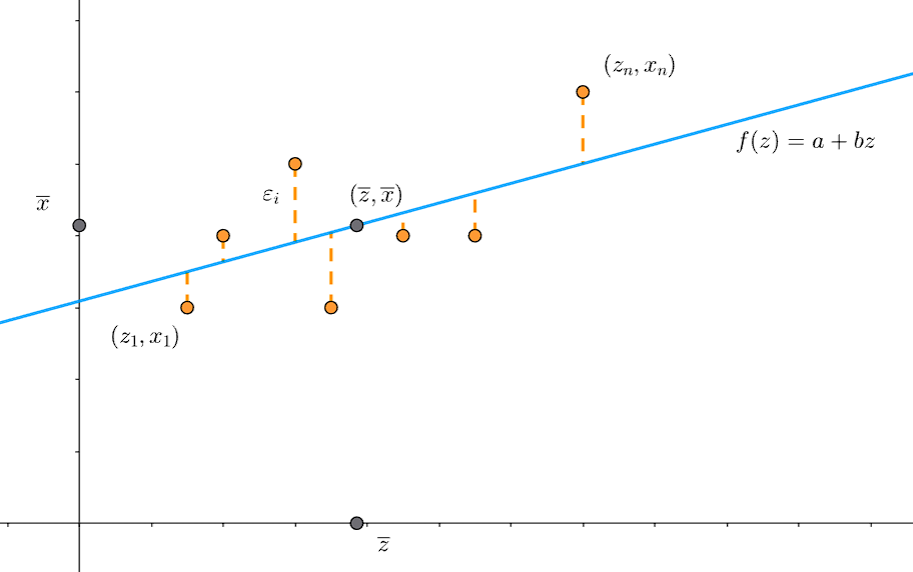
\includegraphics[height=9cm]{mathstat/images/mathstat_2025_04_08_1}
\end{center}

Суть МНК: находим такую прямую, чтобы сумма квадратов длин этих отрезков (по сути отклонений) была минимальна 
(или дисперсия экспериментальных данных относительно прямой была минимальна)


\subsubsection{Выборочный коэффициент линейной корреляции}

\Def $\hat r = \frac{\overline{z x} - \overline{x} \, \overline{z}}{\hat \sigma_z \hat \sigma_x}$ называется выборочным коэффициентов 
линейной корреляции. Ясно, что она будет точечной оценкой теоретического коэффициента линейной корреляции. 
Также $\hat r$ является несмещенной оценкой

Поэтому выборочный коэффициент корреляции характеризует силу линейной связи. Знак коэффициента показывает направления корреляции (прямая или обратная)

Силу связи можно примерно оценить от шкале Чеддока:

\smallvspace

\begin{tabular}{c|l}
    Количественная мера $\hat r$ & Качественная мера \\
    \hline
    $0.1 \ \textendash \ 0.3$ & Слабая \\
    $0.3 \ \textendash \ 0.5$ & Умеренная \\
    $0.5 \ \textendash \ 0.7$ & Заметная \\
    $0.7 \ \textendash \ 0.9$ & Высокая \\
    $> 0.9$ & Весьма высокая \\
\end{tabular}

\mediumvspace

\subsection{Проверка гипотезы о значимости выборочного коэффициента корреляции}

Пусть $(Z, X)$ распределена нормально. По выборке объема $n$ вычислен выборочный коэффициент корреляции $\hat r$, а $r$ - теоретический коэффициент корреляции

Проверяется $H_0 : r = 0$ (выборочный коэффициент корреляции статистически незначим) против $H_1 : r \neq 0$ (коэффициент статистически значим)

\begin{MyTheorem}
    Если $H_0$ верна, то $K = \frac{\hat r \sqrt{n - 2}}{\sqrt{n - \hat r^2}} \in T_{n - 2}$ - распределение Стьюдента с степенью $n - 2$ 
\end{MyTheorem}

Получаем критерий. Пусть $t_\alpha$ - квантиль $|T_{n - 2}|$ (двухстороннее распределение Стьюдента) уровня $\alpha$

\begin{cases}
    H_0 : r = 0, & \text{ если } |K| < t_\alpha \\
    H_1 : r \neq 0, & \text{ если } |K| \geq t_\alpha \\
\end{cases}

Надо понимать, что корреляция - более тонкое понятие, чем зависимость

А термин \textit{регрессия} получил свое название чисто исторически: статистик Гальтон в 1886 году 
исследовал зависимость роста детей от роста родителей

$E(\text{Р}_\text{сына} | Z_\text{отца} = Z_1, Z_\text{матери} = Z_1) = 0.27 Z_1 + 0.2 Z_2 + \operatorname{const}$

$E(\text{Р}_\text{дочери} | Z_\text{отца} = Z_1, Z_\text{матери} = Z_1) = \frac{1}{1.08} \text{Р}_\text{сына}$

Дальше он заметил, что при у самых высоких родителей рост детей был меньше относительно них (скатывался к среднему, происходил регресс)

Позже исследовали экономические результаты фирм, показатели спортсменов, которые после успешного сезона уменьшались, 
после чего появлялось куча теорий. Сейчас все это объясняется простым случаем

\subsection{Выборочное корреляционное отношение}

Выборочный коэффициент корреляции характеризует только силу линейной связи. Следующий подход основан на однофакторном дисперсионном анализе

Пусть есть $k$ выборок случайной величины $X$ при $k$ различных уровнях фактора $Z$. Вычислены общая, внутригрупповая и межгрупповая дисперсии. 
По теореме $D_\text{О} = D_\text{М} + D_\text{В}$

\Def Выборочным корреляционным отношением $X$ на $Z$ называется величина $\eta_{X, Z} = \sqrt{\frac{D_\text{М}}{D_\text{О}}}$

\underline{Свойства}:

\begin{enumerate}
    \item $0 \leq \eta_{X, Z} \leq 1$ ($D_\text{М}, D_\text{О} \geq 0$)

    \item Если $\eta = 1$, то $D_\text{М} = D_\text{О} \Longrightarrow D_\text{В} = 0$, имеем функциональную зависимость $X$ от $Z$

    \item Если $\eta = 0$, то $D_\text{М} = 0 \Longrightarrow$ корреляция отсутствует

    \item $\eta \geq |\hat r|$

    \item Если $\eta = |\hat r|$, то все точки экспериментальных данных лежат на прямой линейной регрессии 
    (то есть данная линейная модель является идеальной)

\end{enumerate}

% end mathstat_2025_04_08.tex

% begin mathstat_2025_04_15.tex





\section{Лекция 10.}

\subsection{Свойство ковариации}

\Mem Ковариацией случайных величин $X$ и $Y$ называется величина $\cov (X, Y) = E((X - EX)(Y - EY)) = E(XY) - EX \cdot EY$

Ковариация является индикатором наличия направления связи между двумя случайными величинами

Пусть имеется $(X_1, Y_1), \dots, (X_n, Y_n)$ случайных величин $X$ и $Y$

\Def Выборочной ковариацией называется величина $\samplecov (X, Y) = \overline{xy} - \overline{x} \cdot \overline{y}$

По Закону Больших Чисел ясно, что $\samplecov (X, Y) \longrightarrow \cov (X, Y)$, поэтому выборочная ковариация является оценкой

\begin{MyTheorem}
    \Ths Выборочная ковариация является точечной состоятельной, но смещенной оценкой ковариации. 
    Несмещенной оценкой будет $\frac{n}{n - 1} \samplecov (X, Y)$
\end{MyTheorem}

Ковариация и выборочная ковариация обладают свойствами

\begin{enumerate}
    \item $\cov (X, Y) = \cov (Y, X)$
    \item $\cov (X, a) = 0$, где $a = \const$
    \item $\cov (X, bY) = b \cov (X, Y)$
    \item $\cov (X + Y, Z) = \cov (X, Z) + \cov (Y, Z)$
    \item $\cov (X, X) = D(X), \samplecov (X, X) = D^* (X)$
    \item $D(X + Y) = DX + DY + 2\cov (X, Y)$
\end{enumerate}

\Nota В дальнейшем под $\cov (X, Y)$ будет пониматься выборочная ковариация

\subsection{Анализ модели линейной парной регрессии}

Пусть при $n$ экспериментах получены значения случайных величин $X$ и $Z$: $(X_1, Z_1), \dots, (X_n, Z_n)$

Пусть $X = \alpha + \beta Z + \varepsilon$ - теоретическая модель линейной регрессии, где $\varepsilon$ - случайная величина,
отражающая влияние невключенных факторов, нелинейность модели, ошибок измерений и просто случая.

Пусть построили с помощью метода наименьших квадратов выборочное уравнение линейной регрессии $\hat X = a + b Z$

Обозначим $\hat \varepsilon_i = X_i - \hat X_i$ - экспериментальная ошибка, разница между наблюдаемыми значениями и 
вычисляемыми по модели

Тогда $X_i = \hat X_i + \hat \varepsilon_i$ или $X_i = a + b Z_i + \hat \varepsilon_i$, где $a$ и $b$ - точечные оценки параметров $\alpha$ и $\beta$

Свойства $\hat \varepsilon_i$:

\begin{enumerate}
    \item $\overline{\hat \varepsilon_i} = 0$

    \begin{MyProof}
        $a = \overline{X} - b \overline{Z} \Longrightarrow a + b \overline{Z} = \overline{X} \Longrightarrow \overline{\hat \varepsilon_i} = \overline{X_i - (a + b Z_i)} = \overline{X} - \overline{a + b Z_i} = \overline{X} - \overline{X} = 0$
    \end{MyProof}

    \item $\cov (\hat X, \hat \varepsilon) = 0$

    \begin{MyProof}
        $b = \overline{\overline{xz} - \overline{x} \cdot \overline{z}}{\hat \sigma^2_z} = \overline{\cov (X, Z)}{D(Z)} \Longrightarrow \cov (X, Z) - b D(Z) = 0$

        $\cov (\hat X, \hat \varepsilon) = \cov (a + b Z, X - a - bZ) = \cov (bZ, X - bZ) = \cov (bZ, x) - \cov (bZ, bZ) = b \cov (Z, X) - b^2 D(Z) = b (\cov (Z, X) - b D(Z)) = 0$
    \end{MyProof}
\end{enumerate}

\subsection{Анализ дисперсии результата}

\Def $D(X) = \frac{1}{n} \sum_{i = 1}^n (X_i - \overline{X})^2$ - дисперсия наблюдаемых значений

\Defs $\hat D(X) = \frac{1}{n} \sum_{i = 1}^n (\hat X_i - \overline{X})^2$ - дисперсия расчетных значений

\Defs $D(\hat \varepsilon) = \frac{1}{n} \sum_{i = 1}^n (\hat \varepsilon_i)^2$ - дисперсия остатков

Так как $X = \hat X + \hat \varepsilon$, $\cov (\hat X, \hat \varepsilon) = 0$, то $D(X) = D(\hat X) + D(\hat \varepsilon) + 2\cov (\hat X, \hat \varepsilon) = D(\hat X) + D(\hat \varepsilon)$

\begin{MyTheorem}
    \Ths $D(X) = D(\hat X) + D(\hat \varepsilon)$
\end{MyTheorem}

Очевидно, что качество модели будет тем лучше, чем меньше будет дисперсия остатков

\Def Коэффициентом детерминации $R^2$ называется величина $R^2 = \frac{D(\hat X)}{D(X)}$ или $R^2 = 1 - \frac{D(\hat \varepsilon)}{D(X)}$

\Notas Смысл $R^2$ - доля объясненной дисперсии, а $1 - R^2$ - доля необъясненной дисперсии

Свойства: 

\begin{enumerate}
    \item $0 \leq R^2 \leq 1$
    \item Если $R^2 = 1$, то $D(\hat \varepsilon) = 0 \Longrightarrow \hat \varepsilon_i = \overline{\hat \varepsilon_i} = 0$, то есть точки лежат строго на 
    линии регрессии, модель идеальна

    \item Если $R^2 = 0$, то $D(\hat X) = 0 \Longrightarrow \hat X = \overline{x}$, то есть получаем примитивную, ничего не объясняющую модель
\end{enumerate}

Чем больше $R^2$, тем лучше качество модели

\subsection{Проверка гипотезы о значимости уравнения регрессии}

Проверяется $H_0 : R^2_\text{теор} = 0$ (уравнение регрессии статистически не значимо) против $H_1 : R^2_\text{теор} \neq 0$

\begin{MyTheorem}
    \Ths Если $H_0$ верна, то $F = \frac{R^2 (n - 2)}{1 - R^2} \in F(1, n - 2)$
\end{MyTheorem}

Пусть $t_\alpha$ - квантиль $F(1, n - 2)$ уровня $\alpha$, тогда:

\begin{cases}
    H_0 : R^2_{\text{теор}} = 0 & \text{ если } F < t_\alpha \\
    H_0 : R^2_{\text{теор}} \neq 0 & \text{ если } F \geq t_\alpha \\
\end{cases}

\Nota Если $H_0 : R^2_{\text{теор}} = 0$, то $H_0 : \beta = 0$

\subsection{Связь между коэффициентом детерминации и коэффициентом линейной корреляции}

\begin{enumerate}
    \item $\sqrt{R^2} = r_{\hat X, X}$ - коэффициент корреляции между $\hat X$ и $X$
    \begin{MyProof}
        $r_{\hat X, X} = \frac{\cov (\hat X, X)}{\sqrt{D(\hat X) D(X)}} = \frac{\cov (\hat X, \hat X + \hat \varepsilon)}{\sqrt{D(\hat X) D(X)}} = 
        \frac{D(\hat X) + \cancelto{0}{\cov (\hat X, \hat \varepsilon)}}{\sqrt{D(\hat X) D(X)}} = \sqrt{\frac{D(\hat X)}{D(X)}} = R$
    \end{MyProof}

    \item $r_{\hat X, X} = |r_{X, Z}|$

    \begin{MyProof}
        $\cov (\hat X, X) = \cov (a + bZ, X) = b \cov (Z, X)$

        $D(\hat X) = D(a + b Z) = b^2 D(Z)$

        $r_{\hat X, X} = \frac{\cov (\hat X, X)}{\sqrt{D(\hat X) D(X)}} = \frac{b \cov (Z, X)}{\sqrt{b^2 D(Z) D(X)}} = \left|\frac{\cov (X, Z)}{\sqrt{D(Z) D(X)}}\right| = |r_{X, Z}|$
    \end{MyProof}
\end{enumerate}

Следствие 1: в случае линейной парной регрессии коэффициент детерминации равен квадрату коэффициенту корреляции

Следствие 2: в случае линейной парной регрессии совпадают результаты проверки гипотез 
$H_0 : R^2_{\text{теор}} = 0 \Longleftrightarrow H_0 : r = 0 \Longleftrightarrow H_0 : \beta = 0$

\subsection{Теорема Гаусса-Маркова}

\begin{MyTheorem}
    \Ths Пусть $X_i = \alpha + \beta Z_i + \varepsilon_i$ - теоретическая модель регрессии

    $X = a + b Z$ - модель, полученная по методу наименьших квадратов

    Если выполнено условия:

    \begin{enumerate}[label=\asbuk*),ref=\asbuk*]
        \item Случайные члены $\varepsilon_i$ независимые случайные величины, имеющие одинаковое нормальное распределение $\varepsilon_i \in N(0, \sigma^2)$
        \item Случайные величины $\varepsilon_i$ и $Z_i$ - независимы
    \end{enumerate}

    Тогда $a$ и $b$ - состоятельные, несмещенные, эффективные оценки параметров $\alpha$ и $\beta$, то есть

    \begin{enumerate}
        \item Состоятельность: $a \underset{n \to \infty}{\ConvergesInProbability} \alpha, b \underset{n \to \infty}{\ConvergesInProbability} \beta$
        \item Несмещенность: $Ea = \alpha, Eb = \beta$
        \item Наименьшая дисперсия, равная:

        $D a = \frac{\overline{z^2} \sigma^2}{n D(Z)}, Db = \frac{\sigma^2}{n D(Z)}$
    \end{enumerate}
\end{MyTheorem}

\Nota Если не выполняется условие а), то есть ошибки зависимы или имеют разную дисперсию, то оценки становятся неэффективными. 
Если не выполнено условие б), то оценки становятся смещенными и несостоятельными

\subsection{Стандартные ошибки коэффициентов регрессии}

Из теоремы видим, что $Da$ и $Db$ зависят от дисперсии $\sigma^2$ случайного члена. 
По экспериментальным ошибкам получаем оценку данной дисперсии:

$D(\hat \varepsilon) = \frac{1}{n} \sum_{i = 1}^n {\hat \varepsilon_i}^2 \underset{n \to \infty}{\ConvergesInProbability} \sigma^2$

Однако эта оценка является смещенной:

$E(D(\hat \varepsilon)) = \frac{n - 2}{n} \sigma^2$

Поэтому несмещенной оценкой дисперсии $\sigma^2$ является величина $S^2 = \frac{1}{n - 2} \sum_{i = 1}^n {\hat \varepsilon_i}^2$

\Def Величина $S$ называется стандартной ошибкой регрессии

Смысл: характеризует разброс наблюдаемых значений вокруг линии регрессии

\Nota Заменим в теореме Гаусса-Маркова $\sigma^2$ на $S^2$, получаем оценки дисперсий $Da$ и $Db$: $S_a^2 = \frac{\overline{z^2} S^2}{n D(z)}, S^2_b = \frac{S^2}{n D(Z)}$

\Def $S_a$ и $S_b$ называются стандартным ошибками коэффициентов регрессии

\subsection{Прогнозирование регрессионных моделей}

Пусть $X = \alpha + \beta Z + \varepsilon$ - теоретическая модель

$\hat X = a + b Z$ - модель МНК, построенная по выборке объема $n$

С помощью данной модели надо дать прогноз значения $X_p$ при заданном значении $Z_p$ и оценить качество прогноза 

Теоретическое значение - $X_p = \alpha + \beta Z_p + \varepsilon$, а точечный прогноз $\hat X_p = a + b Z_p$

Разность между ними $\Delta_p = \hat X_p - X_p$ называется ошибкой предсказания

Свойства $\Delta_p$:

\begin{enumerate}
    \item $E \Delta_p = 0$
    \item $D (\Delta_p) = \left(1 + \frac{1}{n} + \frac{(Z_p - \overline{z})^2}{n DZ}\right) \sigma^2$

    Заменив $\sigma^2$ на $S^2$, получим стандартную ошибку прогноза: $S_{\Delta_p} = S \sqrt{1 + \frac{1}{n} + \frac{(Z_p - \overline{z})^2}{n DZ}}$

    \item $D(\Delta_p) > \sigma^2$ - то есть точность прогноза ограничена случайным членом $\varepsilon$

    \item При $n \to \infty$ $D(\Delta_p) \ConvergesInProbability \sigma^2$ - качество модели тем лучше, чем больше объем выборки

    \item Чем больше $Z_p$ отклоняется от $\overline{z}$, тем хуже качество прогноза. Наилучшее качество в точке $Z_p = \overline{z}: \ D(\Delta_p) = \left(1 + \frac{1}{n}\right) \sigma^2$

    % https://www.geogebra.org/calculator/brxkjkqc

    \begin{center}
        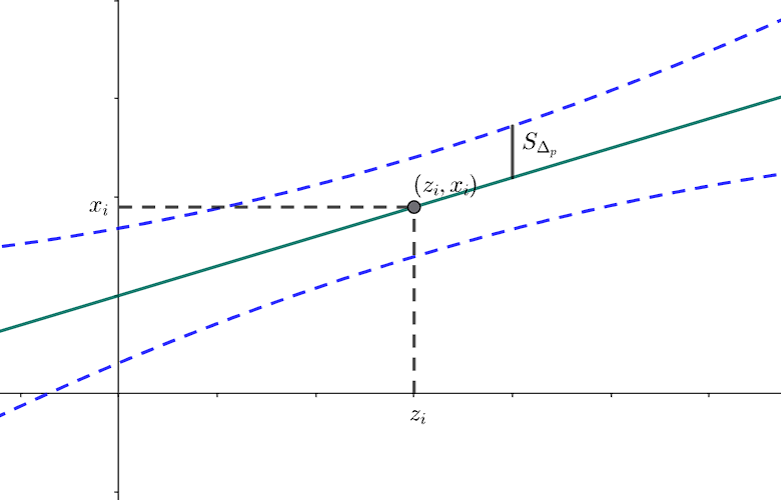
\includegraphics[width=10cm]{mathstat/images/mathstat_2025_04_15_1}
    \end{center}
\end{enumerate}

\subsection{Доверительные интервалы прогноза и коэффициентов уравнения линейной регрессии}

Пусть $t_\gamma$ - квантиль $|T_{n - 2}|$ уровня $\gamma$

Тогда доверительные интервалы надежности $\gamma$ для параметров $\alpha$ и $\beta$:

$\qquad \alpha: (a - t_\gamma S_a; a + t_\gamma S_a)$

$\qquad \beta: (b - t_\gamma S_b; b + t_\gamma S_b)$

Доверительный интервал для прогноза $X_p: (\hat X_p - t_\gamma S_{\Delta_p}; \hat X_p + t_\gamma S_{\Delta_p})$


% end mathstat_2025_04_15.tex

% begin mathstat_2025_04_22.tex





\section{Лекция 11.}

\subsection{Математическое ожидание и дисперсия случайного вектора}

\Def $E \vec X = \begin{pmatrix}E X_1 \\ \vdots \\ E X_n \end{pmatrix}$ - математическое ожидание случайного вектора

\Def Дисперсией или матрицей ковариаций называется $D \vec X = E ((\vec X - E \vec X) (\vec X - E \vec X)^T )$, 
элементами которой $d_{ij} = \cov (X_i, X_j), d_{ii} = D(X_i)$

\underline{Свойства}:

\begin{enumerate}
    \item $E(A \vec X) = A E \vec X$
    \item $E(\vec X + \vec B) = E \vec X + \vec B$
    \item $D(A \vec X) = A D \vec X A^T$
    \item $D(\vec X + \vec B) = D \vec X$
\end{enumerate}

\subsection{Уравнение общей регрессии}

Пусть результат $X$ зависит от $k$ факторов $Z_1, \dots, Z_k$. Рассматриваем теоретическую модель линейной регрессии:

$X = \beta_1 Z_1 + \beta_2 Z_2 + \dots + \beta_k Z_k + \varepsilon$, где $\vec Z = \begin{pmatrix}Z_1 \\ \vdots \\ Z_k \end{pmatrix}$ - вектор факторов, $\vec \beta = \begin{pmatrix}\beta_1 \\ \vdots \\ \beta_k \end{pmatrix}$ - вектор коэффициентов регрессии

Пусть проведено $n \geq k$ экспериментов, $\vec Z^{(i)} = \begin{pmatrix}Z_1^{(i)} \\ \vdots \\ Z_k^{(i)} \end{pmatrix}$ - значения факторов при $i$-ом эксперименте,
$\vec X = \begin{pmatrix}X_1 \\ \vdots \\ X_n \end{pmatrix}$ - соответствующие значения результатов

Согласно модели:

\begin{cases}
    $X_1 = \beta_1 Z_1^{(1)} + \beta_2 Z_2^{(2)} + \dots + \beta_k Z_k^{(1)} + \varepsilon_1$ \\
    $X_1 = \beta_1 Z_1^{(1)} + \beta_2 Z_2^{(2)} + \dots + \beta_k Z_k^{(1)} + \varepsilon_1$ \\
    \dots \\
    $X_n = \beta_1 Z_1^{(n)} + \beta_2 Z_2^{(n)} + \dots + \beta_k Z_k^{(n)} + \varepsilon_n$
\end{cases}

Или в матричной форме: $\vec X = Z^T \vec \beta + \vec \varepsilon$, 
где $Z = \begin{pmatrix}
    Z_1^{(1)} & Z_1^{(2)} & \dots & Z_1^{(n)} \\ 
    Z_2^{(1)} & Z_2^{(2)} & \dots & Z_2^{(n)} \\ 
    \vdots & \vdots & \ddots & \vdots \\
    Z_k^{(1)} & Z_k^{(2)} & \dots & Z_k^{(n)} \\ 
\end{pmatrix}$ - матрица плана, $\vec \varepsilon$ - вектор теоретических ошибок

Наша цель такова: по данной матрице плана $Z$ и вектора результатов $\vec X$ дать оценки неизвестных параметров регрессии $\beta_i$ 
и параметров распределения ошибки $\varepsilon$

\Nota Заметим, что у данной модели мы не теряем свободный член $b_0$, так как при необходимости можно считать, что первый фактор тождественен единицы. 
То есть первая строка матрица плана будет состоять из единиц

\subsection{Метод наименьших квадратов и нормальные уравнения}

Будем считать, что выполнено условие $\mathrm{Cond. 1}$, что ранг матрицы $\operatorname{rang} Z = k$, то есть все строки матрицы плана независимы

Введем матрицу $A = Z Z^T$. Ее свойства:

\begin{enumerate}
    \item $A$ - квадратная и симметричная
    \item $A$ - положительно определенная
    \item $\exists B = \sqrt{A}$, то есть $B^2 = A$
\end{enumerate}

Пусть $\vec B = \begin{pmatrix}b_1 \\ \vdots \\ b_k\end{pmatrix}$ - вектор оценок $\vec \beta = \begin{pmatrix}\beta_1 \\ \vdots \\ \beta_k\end{pmatrix}$

Тогда эмпирическая модель регрессии $\vec{\hat X} = Z^T \vec B$, 
$\vec \varepsilon_i = X_i - \hat X_i$ - экспериментальная ошибка, или $\vec {\hat \varepsilon} = \begin{pmatrix}\hat \varepsilon_1 \\ \vdots \\ \hat \varepsilon_n\end{pmatrix} = \vec X - Z^T \vec B$ - вектор экспериментальных ошибок

По методу наименьших квадратов подбираем $\vec B$ таким образом, чтобы $L(\vec B) = \sum_{i = 1}^n \hat \varepsilon_i^2 \longrightarrow \min$

$\sum_{i = 1}^n \hat \varepsilon_i^2 = \|\vec{\hat \varepsilon}\|^2 = \| \vec X - Z^T \vec B\|^2$ - квадрат расстояния от точки $\vec X$ до $Z^T \vec B$ в $\Real^n$

$Z^T \vec B$ - точка линейного подпространства, порожденного векторами $Z^T \vec t$, где $\vec t \in \Real^k$

\Nota Согласно $\mathrm{Cond. 1}$ размерность линейной оболочки, порожденной вектором $Z^T \vec t$,  $\dim \langle Z^T \vec t \rangle = k$

Наименьшее расстояние получаем, когда квадрат расстояния от точки $\vec X$ до данного подпространства, а вектор $\vec B$ - проекция вектора $\vec X$ на него

Таким образом, вектор $\vec X - Z^T \vec B$ должен быть ортогонален данному подпространству, то есть скалярное произведение вектора $\vec X$ и всех векторов подпространства равно 0

$(Z^T \vec t, \vec X - Z^T \vec B) = (Z^T \vec t)^T (\vec X - Z^T \vec B) = {\vec t}^T (Z^T)^T (\vec X - Z^T \vec B) = {\vec t}^T Z (\vec X - Z^T \vec B) = 
{\vec t}^T (Z \vec X - Z Z ^T \vec B) = 0 \ \forall \vec t \in \Real^k$

Так как всем векторами подпространства ортогонален только нулевой вектор, то получаем, что $Z \vec X - Z Z^T \vec B = 0$ или $A \vec B = Z \vec X$ - нормальное уравнение (или система нормальных уравнений)

Так как по свойству 2 матрица $A$ невырожденная, то существует обратная, получаем решение системы: $\vec B = A^{-1} Z \vec X$

\subsection{Свойства оценок метода наименьших квадратов}

Добавим еще одно важное условие $\mathrm{Cond. 2}$: теоретические ошибки $\varepsilon_i$ - независимы и имеют одинаковое нормальное распределение $N(0, \sigma^2)$.
То есть $E \vec \varepsilon = \vec 0$, $D \vec \varepsilon = \sigma^2 E_n$ (ковариации равны нулю в силу независимости)

\underline{Свойства}:

\begin{enumerate}
    \item $\vec B - \vec \beta = A^{-1} Z \vec \varepsilon$

    \begin{MyProof}
        $\vec B - \vec \beta = A^{-1} Z \vec X - \vec \beta = A^{-1} Z (Z^T \vec \beta + \vec \varepsilon) - \vec \beta = A^{-1} Z \vec \varepsilon$
    \end{MyProof}

    \item $\vec B$ - несмещенная оценка для вектора $\vec \beta$

    \begin{MyProof}
        $E(\vec B - \vec \beta) = E(A^{-1} Z \vec \varepsilon) = A^{-1} Z E \vec \varepsilon = 0 \Longrightarrow E \vec B = \vec \beta$
    \end{MyProof}

    \item Матрица ковариаций $D \vec B = \sigma^2 A^{-1}$

    \begin{MyProof}
        $D \vec B = D (\vec B - \vec \beta) = D (A^{-1} Z \vec \varepsilon) = A^{-1} Z D \vec \varepsilon A^{-1}^T Z^T = A^{-1} Z \sigma^2 E_n A^{-1}^T Z^T = \sigma^2 A^{-1} (Z Z^T) A^{-1} = \sigma^2 A^{-1}$
    \end{MyProof}

    Следствие: дисперсии оценок $b_i$ можно выразить через $\sigma^2$ и коэффициенты матрицы $A^{-1}$: $D b_i = \sigma^2 (A^{-1})_{ii}$

\end{enumerate}

\subsection{Оценка дисперсии случайного члена}

Обозначим $\hat \sigma^2 = \frac{1}{n} \sum_{i = 1}^n \hat \varepsilon^2_i$. Ясно, что $\hat \sigma^2$ - точечная оценка 
неизвестной дисперсии $\sigma^2$, однако она является смещенной оценкой

\begin{MyTheorem}
    Пусть выполнены $\mathrm{Cond. 1}$ и $\mathrm{Cond. 2}$, тогда $\frac{n \hat \sigma^2}{\sigma^2} \in H_{n - k}$ и не зависит от $\vec B$
\end{MyTheorem}

Так как $\frac{n \hat \sigma^2}{\sigma^2} \in H_{n - k}$, то $E \hat \sigma^2 = \frac{\sigma^2}{n} E \frac{n \hat \sigma^2}{\sigma^2} = \frac{\sigma^2}{n} (n - k) = \frac{n - k}{n} \sigma^2 < \sigma^2$ - смещенная вниз оценка

Тогда несмещенной оценкой будет $S^2 = \frac{n}{n - k} \hat \sigma^2 = \frac{1}{n - k} \sum_{i = 1}^n \hat \varepsilon_i^2$




% end mathstat_2025_04_22.tex

% begin mathstat_2025_04_29.tex





\section{Лекция 12.}

\subsection{Построение и анализ уравнения множественной линейной регрессии}

Постановка задачи: пусть выявлена зависимость результата $X$ от фактора $Z_1, Z_2, \dots, Z_k$

При $n > k$ получены результаты экспериментов $\vec X = (X_1, \dots, X_n)$ при соответствующих значениях факторов $\vec Z^{(j)} = (Z^{(j)}_1, Z^{(j)}_2, \dots, Z^{(j)}_k)$

Предполагаем, что зависимость всех факторов от $X$ линейная. Требуется по данным построить линейную модель, наилучшим образом объясняющую предсказывающую поведение $X$

\subsection{Мультиколлинеарность}

\Def Мультиколлинеарность - наличие линейной связи между всеми или несколькими факторами. Неприятные последствия:

\begin{itemize}
    \item Оценки параметров становятся ненадежными, имеют большие стандартные ошибки и малую значимость.
    Небольшое изменение данных приводит к заметному изменению оценок
    \item Трудно определить изолированное влияние конкретного фактора на результат и выявить смысл данного влияния
\end{itemize}

\Ex Исследовалась зависимость веса от роста и размера обуви. В одной группе студентов модель оказалась такая: 
$X$ - вес, $Z_1$ - рост, $Z_2$ - размер обуви, 

В первой группе уравнение получилось таким: $X - \overline{x} = 0.9(Z_1 - \overline{Z_1}) + 0.1(Z_2 - \overline{Z_2})$

А во второй группе таким: $X - \overline{x} = 0.2(Z_1 - \overline{Z_1}) + 0.8(Z_2 - \overline{Z_2})$

\subsection{Отбор факторов в уравнении регрессии}

Чтобы избавиться от неприятных последствий, нужно отобрать факторы, которые мы в дальнейшем будем учитывать. Для этого строим корреляционную матрицу, состоящую из коэффициентов корреляции между результатом, факторами и факторов между собой 

\smallvspace

$r = \begin{pmatrix}
    1 & r_{X, Z_1} & r_{X, Z_2} & \dots & r_{X, Z_k} \\ 
    r_{X, Z_1} & 1 & r_{Z_1, Z_2} & \dots & r_{Z_1, Z_k} \\ 
    r_{X, Z_2} & r_{Z_2, Z_1} & 1 & \dots & r_{X, Z_k} \\ 
    \vdots & \vdots & \vdots & \ddots & \vdots \\ 
    r_{X, Z_k} & r_{Z_k, Z_1} & r_{Z_k, Z_2} & \dots & 1 \\ 
\end{pmatrix}$

\smallvspace

Алгоритм следующий: 

\begin{enumerate}
    \item Первым берем фактор, имеющий наибольшую корреляцию с результатом
    \item Затем добавляем факторы, которые с одной стороны имеют наибольшую корреляцию с результатом, а с другой стороны наименьшую корреляцию с уже имеющимися факторами
\end{enumerate}

\Ex Для данной корреляционной матрицы лучше всего брать $Z_2$ (фактор имеет лучшую корреляцию с $X$), 
а затем $Z_3$ (этот фактор меньше всего коррелирует с $Z_2$)

\begin{tabular}{c|c|c|c|c}
    & X & Z_1 & Z_2 & Z_3 \\
    X & 1 & - & - & - \\
    Z_1 & 0.81 & 1 & - & - \\
    Z_2 & 0.85 & 0.93 & 1 & - \\
    Z_3 & -0.65 & -0.38 & -0.28 & 1
\end{tabular}

\subsection{Анализ уравнения линейной регрессии}

Пусть $X = \beta_0 + \beta_1 Z_1 + \dots + \beta_k Z_k + \varepsilon$ - теоретическая модель линейной регрессии, $\varepsilon \in N(0, \sigma^2)$ и независимы

По методу наименьших квадратов была построена модель $\hat X = b_0 + b_1 Z_1 + \dots + b_k Z_k$. Тогда $\hat \varepsilon_i = X_i - \hat X_i$ - экспериментальная (или эмпирическая) ошибка

Согласно следствию из теоремы $S^2 = \frac{1}{n - k - 1} \sum_{i = 1}^n \hat \varepsilon_i^2$ - несмещенная оценка $\sigma^2$

\Def Величину $S$ называют стандартной ошибкой регрессии 

Из прошлых лекций знаем, что $D b_i = \sigma^2 (A^{-1})_{ii}$, где $A = Z Z^T$, $Z = (Z:{(i)}_j)$ - матрица плана

Из этого $\hat D b_i = S^2 (A^{-1})_{ii}$ - оценка дисперсии

\Def $S_{b_i} = S \sqrt{(A^{-1})_{ii}}$ - стандартная ошибка коэффициента регрессии $b_i$

\subsection{Уравнение регрессии стандартных масштабов}

\Nota При обычном уравнении линейной регрессии трудно сравнить влияние различных факторов, так как они имеют 
разную природу и разные единицы измерения. Поэтому делают стандартизацию данных. 

Пусть есть выборка $\vec X = (X_1, \dots, X_n)$ объема $n$. Тогда стандартизованный вектор $\vec t_x$ состоит из значений $\frac{X_i - \overline{x}}{\hat \sigma_X}$

Получаем новые данные, которые можем считать новой выборкой стандартизированной случайной величины $\frac{X - EX}{\sigma_X}$ и которая не имеет единиц измерения

Свойства стандартизированных данных:

\begin{enumerate}
    \item $\overline{t_x} = 0$
    \item $D^*_{t_x} = 1$
    \item $r_{x,y} = r_{t_x, t_y} = \overline{t_x t_y}$
    \begin{MyProof}
        $r_{x,y} = \frac{\samplecov(x, y)}{\hat \sigma_x \hat \sigma_y} = 
        \frac{\frac{1}{n} \sum_{i = 1}^n (x_i - \overline{x})(y_i - \overline{y})}{\hat \sigma_x \hat \sigma_y} = 
        \frac{1}{n} \sum_{i = 1}^n \frac{x_i - \overline{x}}{\hat \sigma_x} \frac{y_i - \overline{y}}{\hat \sigma_y} = \overline{t_x t_y}$

        $r_{t_x, t_y} = \overline{t_x t_y}$, так как $\overline{t_x} = \overline{t_y} = 0$, $D^* t_x = D^* t_y = 1$
    \end{MyProof}
\end{enumerate}

В уравнении регрессии данные результата и факторов заменяем на стандартизированные: 

$t_j = \left(\frac{Z^{(j)}_i - \overline{Z^{(j)}}}{\sigma_{Z}^{(j)}}\right)$ - стандартизация $j$-ого фактора, $t_x = \left(\frac{X_i - \overline{X}}{\sigma_X}\right)$ - стандартизация результата

Так как стандартизация - линейная операция, то при соответствующей замене в уравнении получаем линейной уравнение,
называемое уравнением регрессии стандартных масштабов:

$t_x = \gamma_1 t_1 + \gamma_2 t_2 + \dots + \gamma_k t_k$

\Nota Заметим, что $\gamma_0$ (свободный член) равен 0: $\overline{t_j} = 0$, поэтому линия уравнения пройдет через начало координат.
При этом система нормальных уравнений приобретает более простой и наглядный вид:

\smallvspace

\begin{cases}
    $\gamma_1 + r_{Z_1, Z_2} \gamma_2 + \dots + r_{Z_1, Z_k} \gamma_k = r_{Z_1, x}$ \\
    $r_{Z_1, Z_2} \gamma_1 + \gamma_2 + \dots + r_{Z_2, Z_k} \gamma_k = r_{Z_2, x}$ \\
    $\dots$ \\
    $r_{Z_k, Z_1} \gamma_1 + r_{Z_k, Z_2} \gamma_2 + \dots + \gamma_k = r_{Z_k, x}$ \\
\end{cases}

\smallvspace

Или в матричной форме: $r \Gamma = r_x$, где $r$ - корреляционная матрица, $\Gamma$ - столбец коэффициентов регрессии, $r_x$ - столбец из коэффициентов корреляции факторов с результатом

Нормальное уравнение регрессии: $A \vec B = Z \vec X$, где $A = Z Z^T$, $Z$ - матрица плана

Допустим, что все данные стандартизированные, тогда для $i$-ого элемента

$\begin{pmatrix}Z_1^{(i)} & \dots & Z_n^{(i)}\end{pmatrix} \begin{pmatrix}X_1 \\ \vdots \\ X_n\end{pmatrix} = 
\sum_{j = 1}^n Z^{(i)}_j X_j = n \overline{Z^{(i)} X} = n r_{Z_i, X}$

$a_{ij} = \begin{pmatrix}Z_1^{(i)} & \dots & Z_n^{(i)}\end{pmatrix} \begin{pmatrix}Z_1^{(j)} \\ \vdots \\ Z_n^{(j)}\end{pmatrix} = 
\begin{cases}
    n \overline{Z_i Z_j} = \gamma_1 r_{Z_i, Z_j}, & \text{ при } i \neq j \\
    n \overline{Z_i^2} = n D Z_i = n, & \text{ при } i = j
\end{cases}$

Перевод коэффициентов можно выполнять по формулам:

$b_i = \gamma_i \frac{\sigma_X}{\sigma_{Z_i}}; \quad \gamma_i = b \frac{\sigma_{Z_i}}{\sigma_X}$, $b_0 = \overline{x} - \sum_{i = 1}^n b_i \overline{z_i}$

\Ex Уравнение парной линейной регрессии:
$\frac{x - \overline{x}}{\hat \sigma_x} = \hat r \frac{z - \overline{z}}{\hat \sigma_z}$

В стандартных масштабах получаем $t_x = \hat r t_z$

Тогда $\gamma_1 = \hat r$

\subsection{Смысл стандартизированных коэффициентов}

Значение $\gamma_i$ можно трактовать как величину прямого влияния $i$-ого фактора на результат. Остальные слагаемые в $i$-ом уравнении можно трактовать
как величины косвенного влияния остальных факторов 

$r_{Z_i Z_1} \gamma_1 + \dots + \gamma_i + \dots + r_{Z_i Z_k} \gamma_k = r_{Z_i, X}$

Величину $r_{Z_i, X}$ можно рассматривать как сумму прямого и косвенного влияний

\Nota Для измерения тесноты отдельной связи между отдельным фактором и результатом при очищении влиянии других факторов
есть понятие коэффициента частной корреляции. При $k = 2$: $r_{X, Z_1 / Z_2} = \frac{r_{X, Z_1} - r_{X, Z_2} r_{Z_1, Z_2}}{\sqrt{(1 - r_{X, Z_2}^2)(1 - r_{Z_1, Z_2}^2)}}$


\subsection{Коэффициенты детерминации и множественной корреляции}

Допустим, что как и в случае парной линейной регрессии дисперсию результата $X$ можно разложить на объясненную и необъясненную $D(X) = D(\hat X) + D(\hat \varepsilon)$

\Nota В зарубежной литературе используется $\operatorname{RSS} = D(\hat \varepsilon) = \sum \hat \varepsilon_i^2$

\Def Коэффициентом детерминации $R^2$ называется величина $R^2 = 1 - \frac{D(\hat \varepsilon)}{D(X)}$

Его можно трактовать как долю объясненной дисперсии, а $1 - R^2$ - как долю необъясненной

Свойства:

\begin{enumerate}
    \item $0 \leq R^2 \leq 1$
    \item Если $R^2 = 1$, то $D(\hat \varepsilon) = 0$, то есть все данные лежат в гиперплоскости построенного уравнения регрессии
    \item Если $R^2 = 0$, то $D(\hat X) = 0$, то есть все $\hat X_i = \overline{x} \Longrightarrow b_1 = b_2 = \dots = b_k = 0$, то есть модель ничего не объясняет
    \item Чем больше $R^2$, тем лучше
    \item В случае линейного уравнения регрессии $R^2 = \sum_{i = 1}^k \gamma_i r_{Z_i, X}$
\end{enumerate}

\Def Величина $R$ называется коэффициентом множественной корреляции, который показывает силу линейной связи

\subsubsection{Скорректированный коэффициент детерминации}

При добавлении в модель новых факторов $R^2$ как правило увеличивается, хотя не всегда есть смысл добавлять новые факторы. 
Для выяснения того, следует ли это делать, используется скорректированный коэффициент детерминации $\overline{R^2} = 1 - \frac{k - 1}{n - k - 1} \frac{D(\hat \varepsilon)}{D(X)}$, 
где $n$ - число экспериментов, а $k$ - число факторов

\subsection{Проверка гипотез по значимости уравнения регрессии}

\begin{enumerate}[label*=\asbuk*) ]
    \item F-тест: проверка гипотезы о значимости уравнения регрессии в целом 
    $H_0 : R^2_\text{теор} = 0 $ (уравнение регрессии статистически незначимо) против $H_1 : R^2_\text{теор} \neq 0$

    \begin{MyTheorem}
        \Ths Если $H_0 : R^2_\text{теор} = 0$ верна, то $F = \frac{R^2}{1 - R^2} \frac{n - k - 1}{k} \in F(k, n - k - 1)$
    \end{MyTheorem}

    Получаем критерий, называемый F-тестом: $t_\alpha$ - квантиль $F(k, n - k - 1)$ уровня значимости $\alpha$

    \begin{cases}
        H_0 : R^2_\text{теор} = 0, & \text{ если } F < t_\alpha \\ 
        H_0 : R^2_\text{теор} \neq 0, & \text{ если } F \geq t_\alpha
    \end{cases}

    \item T-тест: проверка гипотезы о значимости отдельного коэффициента регрессии 
    $H_0 : \beta_i = 0$ ($b_i$ статистически незначим) против $H_1 : \beta_i \neq 0$

    \begin{MyTheorem}
        \Ths Если $H_0 : \beta_i = 0$ верна, то $T_i = \frac{b_i}{S_{b_i}} \in T_{n - k - 1}$
    \end{MyTheorem}

    
    Получаем критерий, называемый T-тестом: $t_\alpha$ - квантиль двухстороннего распределения Стьюдента $|T_{n - k - 1}|$ уровня значимости $\alpha$

    \begin{cases}
        H_0 : \beta_i = 0, & \text{ если } |T_i| < t_\alpha \\ 
        H_0 : \beta_i \neq 0, & \text{ если } |T_i| \geq t_\alpha
    \end{cases}

    \Nota T-тест служит для отсева несущественных факторов из модели при условии, что все другие факторы включены в модель

    \Notas При мультиколлинеарности возможно, что уравнение имеет высокую значимость, а большинство коэффициентов не проходит T-тест 

    \Notas При применении T-теста убираем только один фактор, далее строим новую модель и для нее опять проводим T-тест. Удаление 2 факторов может привести к неопределенным результатам
\end{enumerate}

% end mathstat_2025_04_29.tex

% begin mathstat_2025_05_06.tex





\section{Лекция 13.}

\subsection{Нормализация регрессионного анализа}

Пусть имеется уравнение общей линейной регрессии $\vec X = Z^T \vec \beta + \vec \varepsilon$, где $n$ - число экспериментов, $\vec X$ - столбец результатов экспериментов, $Z$ - матрица плана, $\vec \beta$ - столбец коэффициентов регрессии, $\vec \varepsilon$ - вектор теоретических ошибок

При этом ранее предполагали, что выполнены условия:

\begin{enumerate}
    \item $\operatorname{Cond. 1}$: Строки $Z$ - независимы
    \item $\operatorname{Cond. 2}$: $\varepsilon_i \in N(0, \sigma^2)$ и независимы
\end{enumerate}

Условие 2 часто нарушается

\subsubsection{Взвешенный метод наименьших квадратов}

Пусть $\varepsilon_i \in N(0, v_i \sigma^2)$ и независимы (то есть дисперсия ошибки зависит от номера наблюдения). Другими словами, $D \vec \varepsilon = \sigma^2 V$, где $V = \operatorname{diag} (v_1, \dots, v_n)$

Логично наблюдениям с меньшей дисперсии ошибки предать больший вес. Пусть вес $w_i = \frac{1}{v_i}$. Домножим обе части уравнения регрессии на $\sqrt{w_i}$, тогда получим $\vec \tilde{X} = \tilde Z^T \vec \beta + \vec \tilde{\varepsilon}$, где $\tilde x_i=  \sqrt{w_i} x_i$, $\tilde Z^{(j)}_i = \sqrt{w_i} Z^{(j)}_i$, $\tilde \varepsilon_i = \sqrt{w_i} \varepsilon_i$

$D \vec \tilde{\varepsilon} = D(\sqrt{w_i} \varepsilon_i) = w_i D \varepsilon_i = \frac{1}{v_i} v_i \sigma^2 = \sigma^2$ - получаем, что $D \vec \tilde{\varepsilon} = \sigma^2 E_n$, то есть стандартную ситуацию

Тогда оценки $\vec b$ будут несмещенными и эффективными

Недостаток у этого метода: нужно знать коэффициенты $v_i$

\Ex Рассмотрим модель линейной парной регрессии без свободного члена $X = \beta_0 Z + \varepsilon$

Теоретическое уравнение $A \vec B = Z \vec X$, где $Z = \left(Z_1, \dots, Z_n\right)$ - матрица плана, $\vec B = \hat \beta_0$, $A = Z Z^T = z_1^2 + \dots + z_n^2$, $Z \vec X = z_1 x_1 + \dots + z_n x_n$

$\sum_{i = 1}^n z^2_i \hat \beta_0 = \sum_{i = 1}^n z_i x_i \Longrightarrow \hat \beta_0 = \frac{\sum_{z_i x_i}}{\sum z^2_i}$ - оценка МНК 

По взвешенному методу наименьших квадратов $\tilde \beta_0 = \frac{\sum w_i z_i x_i}{\sum w_i z_i^2}$ - оценка взвешенного МНК

\ExN{a} Взвешенное среднее

Допустим, что проводим серию измерений \enquote{скоропортящимся} инструментом. При $Z \equiv 1$: $X = \beta_0 + \varepsilon$, $\varepsilon_i \in N(0, v_i \sigma^2), w_i = \frac{1}{v_i}$

Тогда $\hat \beta_0 = \frac{\sum_{i = 1}^n w_i x_i}{\sum_{i = 1}^n w_i}$ - взвешенное среднее

\ExN{б} Повторное наблюдение

Пусть было $n$ серий по $k_i$ наблюдений ($1 \leq i \leq n$). В каждой серии вычислили выборочное среднее $\overline{x_i}$. 
Если $\varepsilon \in N(0, \sigma^2)$, то дисперсия ошибки для каждого выборочного среднего $D\varepsilon_i = \frac{\sigma^2}{k_i}$. Оценка по результатам всех наблюдений будет $\hat \beta_0 = \frac{\sum_{i = 1}^n k_i \overline{x_i}}{\sum_{i = 1}^n k_i}$

\ExN{в} Пропорция

Пусть $X$ - потери тепла в квартире. Основной фактор $Z$ - разница температур снаружи и внутри. Так как при $Z = 0$ $X = 0$, то уравнением регрессии будет $X = \beta_0 Z + \varepsilon$

Логично предположить, что дисперсия ошибки зависит от величины $Z$. Рассмотрим две гипотезы:

\begin{enumerate}
    \item Дисперсия ошибки прямо пропорциональна $Z$: $D\varepsilon_i = C Z_i = \sigma^2 \frac{C Z_i}{\sigma^2}$

    Тогда $w_i = \frac{\sigma^2}{C Z_i}$ и $\hat \beta_0 = \frac{\sum_{i = 1}^n \frac{\sigma^2}{C Z_i} Z_i X_i}{\sum_{i = 1}^n \frac{\sigma^2}{C Z_i} Z_i^2} = \frac{\sum X_i}{\sum Z_i} = \frac{\overline{x}}{\overline{z}}$

    \item Дисперсия ошибки квадратично зависит от $Z$: $D\varepsilon_i = C Z_i^2 = \sigma^2 \frac{C Z_i^2}{\sigma^2}$

    Тогда $w_i = \frac{\sigma^2}{C Z_i^2}$ и $\hat \beta_0 = \frac{\sum_{i = 1}^n \frac{\sigma^2}{C Z_i^2} Z_i X_i}{\sum_{i = 1}^n \frac{\sigma^2}{C Z_i^2} Z_i^2} = \frac{\sum X_i}{\sum Z_i} = \frac{\sum \frac{X_i}{Z_i}}{n} = \overline{\left(\frac{x}{z}\right)}$
\end{enumerate}

\subsection{Коррелированные наблюдения}

Пусть ошибки не только имеют различные дисперсии, но и коррелированны между собой: $\cov (\varepsilon_i, \varepsilon_j) = v_{ij}$

Тогда $D \vec \varepsilon = \sigma^2 V$, где $V = \left(v_{ij}\right)$

Так как матрица ковариаций симметричная и положительно определенная, то существует $\sqrt{V}$. Домножим обе части уравнения регрессии на $\sqrt{V^{-1}}$:

$\vec X = Z^T \vec{\beta} + \vec \varepsilon \ \Big| \ \cdot \sqrt{V^{-1}}$

$\vec \tilde{X} = \tilde Z^T \vec \beta + \varepsilon$, где $\vec \tilde{X} = \sqrt{V^{-1}} \vec X$, $\tilde Z = \sqrt{V^{-1}} Z$, $\vec \tilde{\varepsilon} = \sqrt{V^{-1}} \vec \varepsilon$

Тогда матрица ковариаций нового вектора ошибок будет $D \vec \tilde{\varepsilon} = D(\sqrt{V^{-1}} \vec \varepsilon) = \sqrt{V^{-1}} D \vec \varepsilon \left(\sqrt{V^{-1}}\right)^T = \sigma^2 I_n$

То есть получили классическую ситуацию, когда выполнено $\operatorname{Cond. 2}$ и вектор оценок $\hat \beta_0$ будет несмещенным и эффективным

\subsection{Составление матрицы плана при управляемом эксперименте}

Если строки матрицы плана взять ортогональными, то дисперсии оценки коэффициентов $b_i$ регрессии будут минимальными. Поэтому лучше матрицу плана составлять таким образом:

Дисперсии оценок при этом $D b_i = \sigma^2 A^{-1}_{ii}$. Если $Z$ - ортогональная (не обязательно нормированная), то $A = Z Z^T = E_n$, а $D b_i = \frac{\sigma^2}{Z_i^2}$. Несложно доказать, что во всех других случаях дисперсия будет больше

\subsection{Метод главных осей}

Помимо метода наименьших квадратов существует метод \enquote{главных осей}. Идея следующая: матрицу ковариаций приводим к диагональной форме

В МНК мы минимизируем расстояние отрезков, параллельных оси Oy, а в методе главных осей - перпендикуляр от точки до возможной прямой

Результатом метода главных осей получаем прямую, являющуюся главной осью эллипса, появляющегося из корреляционного облака

\subsection{Нелинейные регрессии}

Помимо общего МНК многие нелинейные зависимости могут быть сведены к линейным при помощи простых приемов

\ExN{а} $X = \alpha + \beta f(Z) + \varepsilon$, где $f(x)$ - известная функция

Тогда можно взять новый фактор $Z^\prime = f(Z)$, свели задачу к стандартной, получаем уравнение $X = \alpha + \beta Z^\prime + \varepsilon$

Пример: $X = \alpha + \beta \ln Z + \varepsilon$, то $Z^\prime = \ln Z$

\ExN{б} $X = \alpha Z^\beta \varepsilon$

Логарифмируем: $\ln X = \ln \alpha + \beta \ln Z + \ln \varepsilon \Longleftrightarrow X^\prime = \alpha^\prime + \beta Z^\prime + \varepsilon^\prime$

\ExN{в} $X = \alpha e^{\beta Z} \varepsilon$

Логарифмируем: $\ln X = \ln \alpha + \beta Z + \ln \varepsilon \Longleftrightarrow X^\prime = \alpha^\prime + \beta Z + \varepsilon^\prime$

\ExN{г} Зависимость в виде полинома: $X = \beta_0 + \beta_1 Z + \beta_2 Z^2 + \dots + \beta_k Z^k$

Введем новые факторы $Z_1 = Z, Z_2 = Z^2, \dots, Z_k = Z^k$

$X = \beta_0 + \beta_1 Z + \beta_2 Z_2 + \dots + \beta_k Z_k$

При этом, чтобы избежать мультиколлинеарность, лучше брать $k < 4$. При больших $k$ получить многочлен большой степени, который сможет гарантировано пройти через все точки - это будет статистически незначимо


\Nota Если из теории мы знаем вид зависимости и подбираем ее под данные, то желательно строить модель как можно проще

\Notas Из построенных моделей предпочтительней та, где коэффициент детерминации больше

\mediumvspace

Построение даже удачной регрессионной модели не означает появление причинно-следственной связи. Исторический пример: исследовалась точность бомбометания от различных условий. Пусть $X$ - точность, $Z_1$ - высота, $Z_2$ - ветер, $Z_3$ - количество истребителей противника

Построили модель $X = \beta_0 + \beta_1 Z_1 + \beta_2 Z_2 + \beta_3 Z_3$ и получили $\hat \beta_3 < 0$ - то есть при большем числе техники противника точность увеличивалась. Оказалось, что не был учтен фактор облачности - при нем $\hat \beta_3 > 0$ и коэффициент детерминации улучшился

Или другой пример: корреляция численности аистов и рождения детей в Голландии XX века оказалась прямой







% end mathstat_2025_05_06.tex

% begin mathstat_2025_05_13.tex





\section{Лекция 14.}

\subsection{Моделирование случайных величин}

\subsubsection{Датчики случайных чисел}

Пусть $\eta \in U(0, 1)$

\Def Члены последовательности $y_1, y_2, \dots, y_n$, которые можно рассматривать как экспериментальные данные случайной величины $\eta$, называются псевдослучайными числами. А устройство или алгоритмы для их получения - датчики (или генераторы) случайных чисел

\begin{enumerate}[label*=\Roman*. ]
    \item Физические датчики

    Примерами физических датчиков может быть секундомер, случайной величиной может быть миллисекунды случайно остановленного секундомер, или европейская рулетка с 36 ячейками для шарика

    Простейшим способом случайное число можно сгенерировать, подбрасывая монету, где за одну сторону принимается 1, а за другую - 0

    \begin{MyTheorem}
        \Ths Случайная величина $\eta \in U(0, 1) \Longleftrightarrow$ разряды $\xi_i$ в ее двоичной записи $\sum_{i = 1}^n 2^{-1} \xi_i$ имеют распределение Бернулли $B_{\frac{1}{2}}$
    \end{MyTheorem}

    Если требуется точность $2^{-n}$, то бросать монету нужно $n$ раз 

    Физические датчики довольно примитивными, однако их значения сложно передавать компьютеру. Также две последовательности случайных чисел могут отличаться при одинаковых условиях

    Знаменитый пример использования физических датчиков - \href{https://www.cloudflare.com/learning/ssl/lava-lamp-encryption/}{использование лавовых ламп компанией Cloudflare} для генерации чисел для использования в шифровании

    \item Таблицы случайных чисел

    Пусть имеется таблица псевдослучайных чисел - результат работы некоторого датчика. Случайным образом выбиралась строка и столбец и, начиная с этого места, выбиралась последовательность случайных чисел

    Такой способ использовался до широкого появления компьютеров и сейчас устарел

    \item Математические датчики

    Обычно математический датчик - это рекуррентная последовательность вида $y_n = f(y_{n - 1})$, однако способ генерации может быть значительно сложнее

    В качестве математического датчика разберем мультипликативный датчик: задается большое число $m$, начальное число $k_0$ и множитель $a$, при этом $m$, $k_0$ и $a$ - взаимно простые

    Последовательность $y_n$ задается по формуле:

    $\begin{cases}
        k_n \equiv a k_{n - 1} (\operatorname{mod} m) & \text{- остаток от деления }ak_{n - 1}\text{ на }m \\
        y_n = \frac{k_n}{m} \in (0, 1)
    \end{cases}$

    Есть рекомендация использовать $m = 2^{31} - 1 = 2147483647$, $a = 630360016$ или $764261123$ (алгоритм Дж. Фишмана и Л. Мура)

    \mediumvspace

    Позднее предложили такой датчик (алгоритм Вичмена-Хилла):

    $a_1 = 171$, $m_1 = 30269$, $a_2 = 172$, $m_2 = 30307$, $a_3 = 170$, $m_3 = 30323$ 

    Члены $y_n^\prime, y_n^{\prime\prime}, y_n^{\prime\prime\prime}$ задаются как мультипликативные датчики, а итоговое значение вычисляется как дробная часть от их суммы: $y_n = \{y_n^\prime + y_n^{\prime\prime} + y_n^{\prime\prime\prime}\}$

    Преимущества: работает быстрее (числа меньше), период датчика - $3 \cdot 10^{13}$, а алгоритма Фишмана и Мура - $2 \cdot 10^9$

    Наблюдателю кажется, что, чем сложнее алгоритм датчика, тем более случайным он кажется

\end{enumerate}

\subsection{Моделирование непрерывного распределения}

\subsubsection{Квантильное преобразование (или метод обратной функции)}

На курсе теории вероятности выражали такую теорему:

\begin{MyTheorem}
    \Ths Пусть $F(x)$ - непрерывная, строго возрастающая функция распределения

    Если случайная величина $\eta \in U(0, 1)$, то $\xi = F^{-1}(\eta)$ имеет функцию распределения $F(x)$
\end{MyTheorem}

\Ex Показательное распределение $E_\alpha$: $F(x) = \begin{cases}0, & x < 0 \\ 1 - e^{-\alpha x}, & x \geq 0\end{cases}$

Обратной к ней функцией будет $x = -\frac{1}{\alpha} \ln (1 - y) \Longrightarrow \xi = -\frac{1}{\alpha} \ln \eta \in E_\alpha$

\Ex Нормальное распределение

Если $\xi \in N(0, 1)$, то $\sigma \xi + a \in N(a, \sigma^2)$, поэтому достаточно уметь моделировать стандартное нормальное распределение

$F(x) = \frac{1}{\sqrt{2\pi}} \int_{-\infty}^x e^{-\frac{z^2}{2}} dz$

Если $\eta \in U(0, 1)$, то $\xi = F^{-1}(\eta) \in N(0, 1)$ (\texttt{НОРМ.СТ.ОБР} в Excel)

\Nota Этот алгоритм простой и универсальный, но не самый эффективный

\subsubsection{Нормальные случайные числа}

\begin{enumerate}[label*=\Roman*. ]
    \item На основе ЦПТ

    Пусть $\eta_i \in U(0, 1)$. Тогда $E\eta = \frac{1}{2}$, $D\eta = \frac{1}{12}$, $S_n = \eta_1 + \dots + \eta_n$ и по ЦПТ:

    $\frac{S_n - nE\eta}{\sqrt{n D\eta}} = \frac{S_n - \frac{n}{2}}{\sqrt{\frac{n}{12}}} \rightrightarrows N(0, 1)$

    Уже при $n = 12$ получается неплохое приближение $S_{12} - 6 \approx N(0, 1)$ 

    \item Точное моделирование пары независимых значений $N(0, 1)$

    \begin{MyTheorem}
        Пусть $\eta_1, \eta_2 \in U(0, 1)$ и независимы. Тогда случайные величины $X, Y \in N(0, 1)$ и независимы:

        $X = \sqrt{-2\ln \eta_1} \cos (2 \pi \eta_2)$

        $Y = \sqrt{-2\ln \eta_1} \sin (2 \pi \eta_2)$
    \end{MyTheorem}
    
    \begin{MyProof}
        Пусть $X, Y \in N(0, 1)$ независимы, тогда плотность $f_{X, Y}(x, y) = f_X(x)f_Y(y) = \frac{1}{2\pi} e^{-\frac{1}{2} (x^2 + y^2)}$

        Перейдем к полярным координатам:

        $x = r \cos \varphi, y = r \sin \varphi, |J| = r$

        Плотность: $f_{\Phi, R}(\varphi, r) = \frac{1}{2\pi} e^{-\frac{1}{2}r^2} r$

        Так как $\varphi \in U(0, 2\pi)$, то $f_{\Phi}(\varphi) = \frac{1}{2\pi}$ и $f_{\Phi, R}(\varphi, r) = \underset{f_\Phi}{\underbrace{\frac{1}{2\pi}}} \cdot \underset{f_R}{\underbrace{r e^{-\frac{1}{2}r^2}}} \Longrightarrow \Phi$ и $R$ - независимы 

        Смоделируем $f_R$ методом обратной функции

        $F_R(r) = \int_0^r r e^{-\frac{r^2}{2}} dr = -\int_0^r r e^{-\frac{r^2}{2}} d\left(-\frac{r^2}{2}\right) = e^{-\frac{r^2}{2}} \Big|_0^r = 1 - e^{-\frac{r^2}{2}} = \eta_1$. Тогда $r = \sqrt{-2\ln \eta_1}$

        Аналогично $F_\Phi(\varphi) = \int_0^\varphi \frac{1}{2\pi} d\varphi = \frac{\varphi}{2\pi} = \eta_2 \Longrightarrow \varphi = 2\pi \eta_2$
    \end{MyProof}

    Такой датчик использует всего три сложных операции (логарифм, корень и косинус) и моделирует нормальное распределение очень точно
\end{enumerate}

\subsubsection{Быстрый показательный датчик}

\begin{MyTheorem}
    \Ths Пусть независимая случайная величина $\eta_1, \eta_2, \dots, \eta_n, \eta_{n+1}, \dots, \eta_{2n - 1} \in U(0, 1)$, $\xi_1, \xi_2, \dots, \xi_{n - 1}$ - упорядоченные значения случайных величин $\eta_{n + 1}, \dots, \eta_{2n - 1}$, $\xi_0 = 0$, $\xi_n = 1$

    Тогда случайная величина $\mu_i = -\frac{1}{\alpha}(\xi_i - \xi_{i - 1}) \ln (\eta_1 \cdot \eta_2 \cdot \dots \cdot \eta_n) \in E_\alpha$ и независимы, $1 \leq i \leq n$
\end{MyTheorem}

Экономим на вычислении значения (считаем логарифм один раз), но теряем при сортировке. Алгоритм оптимален при $n = 3$: $\eta_1, \eta_2, \eta_3, \eta_4, \eta_5 \in U(0, 1)$ и $\eta_4 < \eta_5$, тогда $\mu_1 = -\frac{1}{\alpha} \eta_4 \ln (\eta_1 \eta_2 \eta_3); \mu_2 = -\frac{1}{\alpha} (\eta_5 - \eta_4) \ln (\eta_1 \eta_2 \eta_3); \mu_3 = -\frac{1}{\alpha} (1 - \eta_5) \ln (\eta_1 \eta_2 \eta_3)$

\subsection{Моделирование дискретных случайных величин}

\begin{enumerate}[label*=\Roman*. ]
    \item Общий метод (или квантильное преобразование)

    Пусть $\xi$ - дискретная случайная величина с законом распределения $P(\xi = x_i) = p_i$

    Разбиваем единичный отрезок на отрезки длин $p_1, p_2$ и так далее

    Пусть $r_m = \sum_{i = 1}^m P_i$ - границы отрезков

    Если $\eta_i \in U(0, 1)$ и $\eta_i \in [r_{i-1}, r_{i})$, то $\xi_i = x_i$

    В частности, так можно смоделировать распределение Бернулли: делим отрезок на две части; если $\eta_i < 1 - p$, то $\xi_i = 0$, если $\eta_i \geq 1 - p$, то $\xi_i = 1$

    \item Биномиальное распределение

    $B_{n,p}: P(\xi = k) = C_n^k p^k q^{n - k}$, $k = 0, 1, \dots, n$ - число успехов при $n$ экспериментах
    
    Берем $n$ значений датчика $y_1, \dots, y_n \in U(0, 1)$. Если $y_i < 1 - p$, то $z_i = 0$, если $y_i \geq 1 - p$, то $z_i = 1$

    Тогда $\xi_i = \sum_{i = 1}^n z_i \in B(n, p)$

    \item Геометрическое распределение

    $G_p: P(\xi = k) = p q^{k - 1}$ - номер первого успеха в испытании

    Берем серию значений датчика $y_i \in U(0, 1)$ до тех пор, пока не будет $y_i \geq 1 - p$. Тогда $\xi = i$ - номер эксперимента

    \item Распределение Пуассона

    $\Pi_\lambda: P(\xi = k) = \frac{\lambda^k}{k!} e^{-\lambda}, k = 0, 1, \dots$

    Используем тот факт, что распределения показательное и Пуассона довольно тесно связаны

    \begin{MyTheorem}
        \Ths Пусть $\mu_1, \mu_2, \dots, \mu_n$ - независимые случайные величины с распределением $E_\lambda$

        Пусть $S_n = \mu_1 + \dots + \mu_n, N = \max n$ такое, что $S_N \in [0, 1]$

        Тогда $N \in \Pi_\lambda$
    \end{MyTheorem}

    Алгоритм: проводим серию $k$-ую серию испытаний до тех пор, пока $\prod^k_{i = 1} y_i < e^{-\lambda}$, тогда $\xi_i = k$

\end{enumerate}



% end mathstat_2025_05_13.tex

% begin mathstat_2025_05_20.tex





\section{Лекция 15.}

\subsection{Метод Монте-Карло}

Метод Монте-Карло появился в статье Метрополиса и Улама и был назван в честь района Монте-Карло в Монако, где были расположены элитные казино


Общая постановка задачи: пусть требуется найти неизвестное число $a$ и при этом имеется случайная величина $\xi$ такая, что $E \xi = a$. Тогда по Закону Больших Чисел $\frac{\xi_1 + \dots + \xi_n}{n} \ConvergesInProbability a$ -- то есть при длинном разыгрывании $a^* = \frac{S_n}{n}$

Оценим погрешность метода: если $D\xi_1 < \infty$, то по ЦПТ $\frac{(\xi_1 + \dots + \xi_n) - n a}{\sqrt{n D \xi_1}} = \frac{n \overline{x} - na}{\sqrt{n D\xi_1}} = \frac{n(\overline{x} - a)}{\sqrt{n D\xi_1}} = \sqrt{n} \frac{\overline{x} - a}{\sqrt{D\xi_1}} \rightrightarrows N(0, 1)$

По правилу \enquote{трех сигм} $P\left(\left|\sqrt{n} \frac{\overline{x} - a}{\sqrt{D\xi_1}}\right| < 3\right) \underset{n \to \infty}{\longrightarrow} 0.9973 \approx 1 \Longrightarrow \sqrt{n} \frac{|\overline{x} - a|}{\sqrt{D \xi_1}} < 3 \Longrightarrow \delta = |\overline{x} - a| < \frac{3\sqrt{D\xi_1}}{\sqrt{n}}$

\Nota То есть скорость сходимости в методе Монте-Карло порядка $\sqrt{n}$ -- довольно медленная, поэтому метод Монте-Карло применяется в ситуации, не требующих высокой точности, где допустима погрешность $5\%$

\subsubsection{Вычисление интегралов}

\Mem $\int_a^b \varphi(x) dx = \lim_{\Delta x \to 0} \sum_{i = 1}^n \varphi(x_i) \Delta x_i$, где $\Delta x_i$ -- длины отрезков разбиения $A_i = [a_i, a_{i + 1}]$, а $x_i \in A_i$

На этом определении построены квадратурные формы:

\begin{enumerate}[label*=\Roman*. ]
    \item Метод прямоугольников

    Отрезок от $a$ до $b$ разбивается на $n$ равных частей $A_i = [a_i, a_{i + 1}]$, $i = 0, 1, \dots, n - 1$

    $x_i = \frac{a_i + a_{i + 1}}{2}$ -- середина интервала

    Тогда $I = \int_a^b \varphi(x) dx \approx \frac{b - a}{n} (y_0 + \dots + y_{n - 1}) = I_n$, где $y_i = \varphi(x_i)$

    Погрешность $|I - I_n| \leq \frac{M_1}{n^2}$, где $M_1$ -- некая константа, зависящая от функции и длины интервала

    \item Формула трапеций

    Идея состоит в том, чтобы вместо площади прямоугольников считать площади трапеций. Отрезок также разбивается на $n$ равных частей

    $y_i = \varphi(x_i)$

    $I = \int_a^b \varphi(x) dx \approx \frac{b - a}{2n} (y_0 + y_n + 2(y_1 + y_2 + \dots + y_{n - 1})) = I_n$

    Здесь погрешность $|I - I_n| < \frac{M_2}{n^2}$, где $M_2 = \frac{M_1}{2}$

    \item Формула Симпсона или формула парабол

    Здесь вместо трапеций будем использовать площадь под параболой, проходящей через 3 точки

    $[a, b]$ разбивается на $n = 2m$ -- четное число равных отрезков

    $I = \int_a^b \varphi(x) dx \approx \frac{b - a}{3n} (y_0 + y_n + 4(y_1 + y_3 + \dots + y_{n - 1}) + 2(y_2 + y_4 + \dots + y_{n - 2})) = I_n$

    Погрешность $|I - I_n| \leq \frac{M_3}{n^4}$ -- намного лучше, чем у предыдущих двух

    \item Метод Монте-Карло

    $I = \int_a^b \varphi(x) dx$

    Так как можно привести отрезок $[a, b]$ к $[0, 1]$ при помощи линейной замены $\frac{x - a}{b - a}$, то ограничимся интегралом $I = \int_0^1 \varphi(x) dx$

    Имеем датчик $\eta_i \in U(0, 1)$, $f_{\eta} (x) = 1, x \in [0, 1]$

    Пусть $\xi_i = \varphi(\eta_i)$, тогда $E\xi_i = \int_{-\infty}^{\infty} \varphi(y) f_\eta (y) dy = \int_0^1 \varphi(y) dy = I$. 
    
    Поэтому $I \approx I_n = \frac{1}{n} \sum_{i = 1}^n \xi_i = \frac{1}{n} (\varphi(\eta_1) + \dots + \varphi(\eta_n))$

    При этом оценка погрешности будет $|I - I_n| \leq \frac{3\sqrt{D \xi_1}}{\sqrt{n}}$, где $D \xi_1 = \int_0^1 \varphi^2(y) dy - I^2$

    Недостатки: медленная скорость сходимости; для оценки погрешности надо оценить дисперсию $D\xi_i$; оценка справедлива лишь с вероятностью

    Поэтому метод Монте-Карло не применяется

\end{enumerate}

\subsubsection{Метод Монте-Карло в кратных интегралах}

\Nota При вычислении $k$-кратных интегралов при помощи квадратурных формул число узлов быстро возрастает как $n^k$, при этом скорость сходимости при больших $k$ будет $\frac{1}{n^{1 + \varepsilon}}$, где $\varepsilon$ - малое число больше 0. А метод Монте-Карло по-прежнему дает скорость сходимости $\frac{1}{\sqrt{n}}$, при этом всего лишь достаточно набросать $n$ случайных точек в данную область

$I = \iint \dots \int_D \varphi(x_1, x_2, \dots, x_k) dx_1 dx_2 \dots dx_k$

По методу Монте-Карло $I \approx \frac{1}{n} \sum_{i = 1}^n \varphi(y_1, \dots, y_k) \cdot I_D$, где $y_1, \dots, y_n$ - значения датчика случайных чисел, а $I_D$ - индикатор, который равен 1, если $(y_1, \dots, y_k) \in D$ (считаем, что $D \subset [0, 1]^k$, а $(y_1, \dots, y_k) \in [0, 1]^k$) 

\Ex Вычислим площадь четверти круга $x^2 + y^2 = 1, x \geq 0, y \geq 0$

Тогда генерируем случайные точки в квадрате $[0, 1]^k$, получаем $n$ точек, из которых $n_D$ входит в круг. Тогда площадь четверти $S_D = \frac{\pi}{4} \approx \frac{n_D}{n} \Longrightarrow \pi = \frac{4}{n_D}{n}$

\subsection{Метод Монте-Карло расслоенной выборки}

Пусть $I = \int_0^1 \dots \int_0^1 \varphi(x_1, \dots, x_k) dx_1 \dots dx_k$

Каждую из сторон куба разобьем на $N$ равных частей, тогда куб разобьется на $n = N^k$ равных кубиков. В каждом из этих кубиков возьмем случайную точку $\eta_i = (\eta_i^{(1)}, \dots, \eta_i^{(k)})$, $1 \leq i \leq n$

Тогда $I \approx I_n = \frac{1}{n} \sum_{i = 1}^n \varphi(\eta_i)$

При этом методе погрешность будет лучше: $|I - I_n| \leq \frac{C}{n^{\frac{1}{2} + \frac{1}{k}}}$

Например, при $I = \int_0^1 \varphi(x) dx$ погрешность $|I - I_n| \leq \frac{C}{n^\frac{3}{2}}$

\subsection{Равномерность по Вейлю}

\Def Числовая последовательность $x_1, x_2, \dots, x_n, \dots, x_i \in [0, 1]$ называется равномерной по Вейлю, если частота попадания точек на любой отрезок $[a, b] \subset [0, 1]$ стремится к его длине $\frac{b - a}{1}$

В частности значения случайной величины $\xi \in U(0, 1)$ обладают данным свойством согласно Закону Больших Чисел, как и значения датчиков случайных чисел 

\begin{MyTheorem}
    \Ths Пусть $x_n = \{n \cdot \alpha\}$ -- дробная часть, где $\alpha$ -- иррациональное число. Тогда последовательность $x_n$ является равномерной по Вейлю
\end{MyTheorem}

Если $x_n$ равномерна по Вейлю, то $I_n = \frac{1}{n} \sum_{i = 1}^n \varphi(x_i) \longrightarrow I = \int_0^1 \varphi(x) dx$

\Nota Но если $x_n$ равномерна по Вейлю, то возможно, что $I_n = \frac{1}{n} \sum_{i = 1}^n \varphi(x_i, x_{i + 1}) \not\longrightarrow I = \int_0^1 \int_0^1 \varphi(x, y) dx dy$, так как соседние члены последовательности будут не такими случайными, как в датчике случайных чисел 

\Def Числовая последовательность $x_1, \dots, x_n$, $x_i \in [0, 1]$ называется вполне равномерной, если для любого $k \in \Natural$ частота попадания $k$-мерных точек $(x_{(n - 1) k + 1}, \dots, x_{nk})$ в любой $k$-мерный параллелепипед внутри $[0, 1]^k$ стремится к объему параллелепипеда

\begin{MyTheorem}
    \Ths Чемпернауна

    Для числа $0.1234567891011121314151617\dots$ подпоследовательность цифр будет вполне равномерной (то есть каждая последовательность чисел встречается примерно так же часто, как и все другие последовательности чисел той же длины)
\end{MyTheorem}

Парадокс первой цифры: являются ли все первые цифры в записи числа $2^n$ равновероятными

Пусть $m = 1, 2, 3, \dots, 9$ равновероятны ($p = \frac{1}{9}$)

Пусть $m$ - первый цифра $2^n$. Тогда $m \cdot 10^l \leq 2^n < (m + 1) \cdot 10^l$

Прологарифмируем: $l + \log_{10} m \leq n \log_{10} 2 < l + \log_{10} (m + 1)$

$\log_{10} m \leq \{n \log_{10} 2\} < \log_{10} (m + 1)$

Число $\{n \log_{10} 2\}$ -- иррациональное, поэтому последовательность будет равномерной по Вейлю, поэтому $p(m) = \log_{10} (m + 1) - \log_{10} m = \log_{10} \left(1 + \frac{1}{m}\right)$

Например, при $m = 7, p(7) \approx 0.058 \neq \frac{1}{9}$

% end mathstat_2025_05_20.tex

% begin mathstat_exam_list.tex
\clearpage

\section{X. Программа экзамена в 2024/2025}


\begin{enumerate}
    \item Выборочная функция распределения. Теоремы Гливенко-Кантелли и Колмогорова.

    \Def \hyperlink{selective_distribution_function}{Выборочной функцией распределения} $F^*(x)$ называется функция 
    
    $F^*(x) = \frac{\text{число данных } x_i < x}{n}$

    \begin{MyTheorem}
        \Ths Выборочная функция распределения поточечно сходится к теоретической функции распределения:

        \[\forall y \in \Real F^*(y) \overset{p}{\longrightarrow} F(y)\]
    \end{MyTheorem}

    \begin{MyTheorem}
        \ThNs{Гливенко-Кантелли} $\sup_{x \in \Real} |F^*(x) - F(x)| \overset{p}{\longrightarrow} 0$
    \end{MyTheorem}

    \begin{MyTheorem}
        \ThNs{Колмогорова} $\sqrt{n} \sup_{x \in \Real} |F^*(x) - F(x)| \rightrightarrows K$ - распределение Колмогорова с 
        функцией распределения $F_K(x) = \sum_{j = -\infty}^{\infty} (-1)^j e^{-2 j^2 x^2}, \ x \in [0;\infty)$
    \end{MyTheorem}

    \item Вариационный и интервальный вариационный ряды. Полигон и гистограмма, ее свойства.

        
    \hyperlink{initial_data_processing}{Начальная обработка статданных}

    \begin{enumerate}
        \item Ранжирование данных - упорядочиваем выборки по возрастанию. В результате получаем вариационный ряд $\vec{X} = (X_{(1)}, X_{(2)}, \dots, X_{(n)})$

        $X_{(1)} = \min X_i; \quad X_{(n)} = \max X_i$

        $X_{(i)} = i$-ая порядковая статистика

        \item Объединим повторяющиеся данные - получаем т.н. частотный вариационный ряд

        \begin{tabular}{c|c|c|c|c}
            $X_i$ & $X_{(1)}$ & \dots & $X_{(r)}$ & $\sum$ \\ 
            \hline
            $n_i$ & $n_1$ & \dots & $n_r$ & $n$ \\ 
        \end{tabular}

        Иногда часть данных отбрасывается сверху и снизу (по 5, по 10, по 5\% и так далее), чтобы сделать выборку репрезентативной

        Тогда $\overline{x} = \frac{1}{n} \sum X_i n_i$, $D^* = \frac{1}{n} \sum (X_i - \overline{x})^2 n_i$
        
        \item Чтобы уменьшить количество вычислений или сделать гистограмму, делают интервальный вариационный ряд: 
        разбиваем данные на интервалы и считаем, сколько данных $n_i$ попало в интервал. 

        Тогда $n_i$ - частота интервала $A_i$

        Есть два основные способа разбиения на интервалы: 

        \begin{enumerate}
            \item Интервалы одинаковой длины
            \item Равнонаполненные интервалы (в каждом интервале примерно одинаковое количество данных)
        \end{enumerate}

        Число интервалов $K$ такое, что $\frac{K(n)}{n} \longrightarrow 0$ и $K(n) \underset{n \to \infty}{\longrightarrow} \infty$

        Обычно применяют формулу Стерджесса $K \approx 1 + \log_2 n$ или $K \approx \sqrt[3]{n}$

        Пусть получили интервальный вариационный ряд

        \begin{tabular}{c|c|c|c|c|c}
            интервалы & $[a_0; a_1)$ & $[a_1; a_2)$ & \dots & $[a_{K - 1}; a_K]$ & $\sum$ \\ 
            \hline
            частоты & $n_1$ & $n_2$ & \dots & $n_K$ & $n$ \\ 
        \end{tabular}
    \end{enumerate}

    \smallvspace
        
    \begin{multicols}{2}
        \begin{itemize}
            \item Гистограмма

            Строится ступенчатая фигура из прямоугольников, основание $i$-ого прямоугольника - интервал, 
            высота прямоугольника - $\frac{n_i}{n l_i}$, где $l_i$ - длина интервала. 
            Визуально можно сделать гипотезу, как ведет себя распределение. 

            \begin{center}
                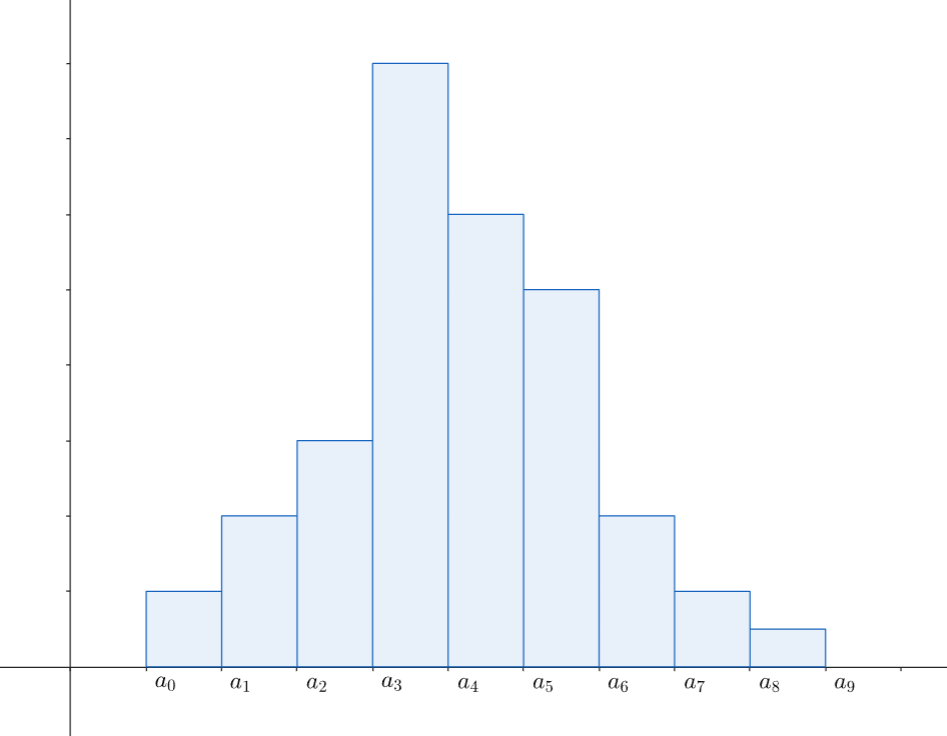
\includegraphics[width=0.4\textwidth]{mathstat/images/mathstat_2025_02_11_1}
            \end{center}

            \item Полигон

            На оси абсцисс отмечаем значения частотного вариационного ряда, по оси ординат - их частоты. 
            Получившиеся точки соединяем отрезками

            \begin{center}
                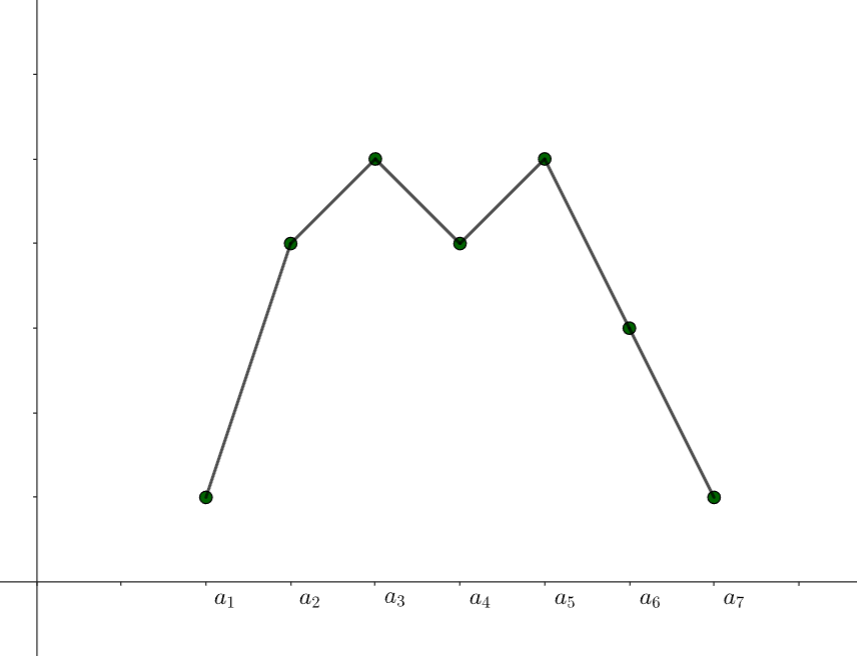
\includegraphics[width=0.4\textwidth]{mathstat/images/mathstat_2025_02_11_2}
            \end{center}
        \end{itemize}
    \end{multicols}

    \item Точечные оценки. Их свойства: состоятельность, несмещенность, эффективность.

    Пусть имеется выборка $\vec{X} = (X_1, X_2, \dots, X_n)$ объемом $n$. Пусть требуется найти приближенную оценку $\theta^*$ неизвестного параметра $\theta$. Находим ее при помощи некоторой функции обработки данных $\theta^* = \theta^*(X_1, \dots, X_n)$
    
    \Defs Такая функция называется статистикой
    
    \Defs А оценка $\theta^*$ называется \hyperlink{point_estimation}{точечной оценкой}

    \Defs Статистика $\theta^* = \theta^*(X_1, \dots, X_n)$ неизвестного параметра называется
    \textbf{состоятельной}, если $\theta^* \overset{p}{\longrightarrow} \theta$ при $n \to \infty$

    \Defs Оценка $\theta^*$ параметра $\theta$ называется \textbf{несмещенной}, если 
    математическое ожидание $E \theta^* = \theta$
        
    \Notas Оценка $\theta^*$ называется асимптотически несмещенной, если 
    $E \theta^* \overset{p}{\longrightarrow} \theta$ при $n \to \infty$

    \Defs Оценка $\theta^*_1$ не хуже $\theta^*_2$, если $E (\theta^*_1 - \theta)^2 \leq E (\theta^*_2 - \theta)^2$.
    Или, если $\theta^*_1$ и $\theta^*_2$ несмещенные, то $D \theta^*_1 \leq D \theta^*_2$

    \Defs Оценка $\theta^*$ называется \textbf{эффективной}, если она не хуже всех остальных оценок

    \Notas Не существует эффективной оценки в классе всех возможных оценок

    \begin{MyTheorem}
        \Ths В классе несмещенных оценок существует эффективная оценка
    \end{MyTheorem}

    \Defs Оценка $\theta^*$ параметра $\theta$ называется асимптотически нормальной, если 
    $\sqrt{n} (\theta^* - \theta) \rightrightarrows N(0, \sigma^2 (\theta))$ при $n \to \infty$

    \item Точечные оценки моментов. Свойства оценок математического ожидания и дисперсии.

    \hyperlink{moments_point_estimation}{Точечные оценки моментов}:

    \Defs Выборочным средним $\overline{x}$ называется величина $\overline{x} = \frac{1}{n} \sum_{i = 1}^n X_i$

    \Defs Выборочной дисперсией $D^*$ называется величина $D^* = \frac{1}{n} \sum_{i = 1}^n (X_i - \overline{x})^2$

    \Defs Исправленной дисперсией $S^2$ называется величина $S^2 = \frac{n}{n - 1} D^* = \frac{1}{n - 1} \sum_{i = 1}^n (X_i - \overline{x})^2$

    \Defs Выборочным средним квадратическим отклонением называется величина $\sigma^* = \sqrt{D^*}$

    \Defs Исправленным средним квадратическим отклонением называется величина $S = \sqrt{S^2}$

    \Defs Выборочным $k$-ым моментом называется величина $\overline{x^k} = \frac{1}{n} \sum_{i = 1}^n X_i^k$

    \Defs Модой $\mathrm{Mo}^*$ называется варианта $x_k$ с наибольшей частотой $n_k = \max_i (n_1, n_2, \dots, n_m)$

    \Defs Выборочной медианой $\mathrm{Me}^*$ называется варианта $x_i$ в середине вариационного ряда $\begin{cases}\mathrm{Me}^* = 
    X_{(k)}, & \text{если } n = 2k - 1 \\ \frac{X_{(k)} + X_{(k + 1)}}{2}, & \text{если } n = 2k\end{cases}$
    
    \begin{MyTheorem}
        \Ths $\overline{x}$ - состоятельная несмещенная оценка теоретического матожидания $EX = a$
    
        1) $E \overline{x} = a$
    
        2) $\overline{x} \overset{p}{\longrightarrow} a$ при $n \to \infty$
    \end{MyTheorem}
    
    \begin{MyTheorem}
        \Ths Выборочный $k$-ый момент является состоятельной несмещенной оценкой теоретического $k$-ого момента
    
        1) $\overline{E X^k} = E X^k$
    
        2) $\overline{X^k} \overset{p}{\longrightarrow} X^k$
    \end{MyTheorem}
    
    \begin{MyTheorem}
        \Ths Выборочной дисперсией $D^*$ и $S^2$ являются состоятельными оценками теоретической дисперсией, при этом $D^*$ - смещенная оценка, а $S^2$ - несмещенная оценка
    \end{MyTheorem}

    \item Метод моментов. Пример.

    \hyperlink{method_of_moments}{Метод моментов}: пусть имеется выборка объема $n$ неизвестного распределения, но известного типа,
    которое задается $k$ параметрами: $\theta = (\theta_1, \theta_2, \dots, \theta_k)$. Требуется дать оценки данным
    неизвестным параметрам

    Идея метода состоит в том, что сначала находим оценки $k$ моментов, а затем с помощью теоретических формул
    из теории вероятности даем оценки этих параметров

    Пусть $\vec{X}$ - выборка из абсолютно непрерывного распределения $F_\theta$ с плотностью известного типа, 
    которая задается $k$ параметрами $f_\theta (x, \theta_1, \dots, \theta_k)$

    Тогда теоретические моменты находим по формуле $m_i = \int_{-\infty}^{\infty} x^i f_\theta (x, \theta_1, \dots, \theta_k) dx = h_i(\theta_1, \dots, \theta_n)$

    Получаем систему из $k$ уравнений с $k$ неизвестными. В эти уравнения подставляем найденные оценки
    моментов и, решая получившуюся систему уравнений, находим нужные оценки параметров

    $\begin{cases}
    \overline{x} = h_1(\theta_1^*, \dots, \theta_n^*) \\ 
    \overline{x^2} = h_2(\theta_1^*, \dots, \theta_n^*) \\ 
    \dots \\
    \overline{x^k} = h_k(\theta_1^*, \dots, \theta_n^*) \\ 
    \end{cases}$

    \Ex Пусть $X \in U(a, b)$. Обработав статданные, нашли оценки первого и второго моментов: $\overline{x} = 2.25; \overline{x^2} = 6.75$

    Нужно найти оценки параметров $a^*, b^*$

    $EX = \int_a^b x \frac{1}{b - a} dx = \frac{a + b}{2}$

    $EX = \int_a^b x^2 \frac{1}{b - a} dx = \frac{a^2 + ab + b^2}{3}$

    Получаем:

    $\begin{cases}
        \overline{x} = \frac{a^* + b^*}{2} \\ 
        \overline{x^2} = \frac{a^*^2 + a^* b^* + b^*^2}{3} \\ 
    \end{cases} \Longleftrightarrow \begin{cases}
        a^* + b^* = 4.5 \\ 
        a^*^2 + a^* b^* + b^*^2 = 20.25 \\ 
    \end{cases} \Longleftrightarrow \begin{cases}
        a^* + b^* = 4.5 \\ 
        a^* b^* = 0 \\ 
    \end{cases} \Longleftrightarrow \begin{cases}
        a^* = 0 \\ 
        b^* = 4.5 \\ 
    \end{cases}$

    \item Метод максимального правдоподобия. Пример.

    \hyperlink{maximum_likelihood_estimation}{Метод максимального правдоподобия}: пусть имеется выборка $\vec{X} = (X_1, \dots, X_n)$ из распределения известного типа, определяемого неизвестными параметрами 
    $\theta = (\theta_1, \dots, \theta_n)$

    Идея метода состоит в следующем: подбираем параметры таким образом, чтобы вероятность получения
    данной выборки при случайном эксперименте была наибольшей.

    Если распределение дискретное, то $P_{\theta} (X_1 = x_1, X_2 = x_2, \dots, X_n = x_n) = P(X_1 = x_1) \dots P(X_n = x_n)$

    \Defs Функцией правдоподобия $L(\vec{X}, \theta)$ называется функция $L(\vec{X}, \theta) = P(X_1 = x_1) \dots P(X_n = x_n) = \prod_{i = 1}^n P(X_i = x_i)$ при дискретном распределении

    и $L(\vec{X}, \theta) = f_\theta(x_1) \dots f_\theta(x_n) = \prod_{i = 1}^n f_\theta(x_i)$ в абсолютно непрерывном распределении

    \Defs Логарифмической функцией правдоподобия называется функция $\ln L(\vec{X}, \theta)$

    \Notas Так как $y = \ln x$ возврастающая функция, точки максимума совпадают, а такую функцию правдоподобия становится легче дифференцировать

    \Defs Оценкой максимального правдоподобия $\hat{\theta}$ называется значение $\theta$, при котором функция правдоподобия 
    $L(\vec{X}, \theta)$ достигает наибольшего значения (при фиксированных значениях выборки)

    \Ex Пусть $\vec{X} = (X_1, \dots, X_n)$ - выборка из распределения Пуассона $\Pi_\lambda$ с неизвестным $\lambda > 0$

    \Mems Для распределения Пуассона $P(X = x_i) = \frac{\lambda^{x_i}}{x_i!} e^{-\lambda}$
    
    Получаем функцию максимального правдоподобия $L(\vec{X}, \lambda) = \prod_{i = 1}^n \frac{\lambda^{x_i}}{x_i!} e^{-\lambda} = 
    \frac{\lambda^{\sum_{i = 1}^n x_i}}{\prod_{i = 1}^n x_i!} e^{-n\lambda} = \frac{\lambda^{n \overline{x}}}{\prod_{i = 1}^n x_i!} e^{-n\lambda}$
    
    $\ln L(\vec{X}, \lambda) = n \overline{x} \ln \lambda - \ln \prod_{i = 1}^n x_i! - n\lambda$
    
    $\frac{\partial \ln L}{\partial \lambda} = \frac{n \overline{x}}{\lambda} - n = 0 \Longrightarrow \hat{\lambda} = \overline{x}$ - оценка максимального правдоподобия
    
    Убедимся, что этот экстремум - максимум: $\frac{\partial^2 \ln L}{\partial \lambda^2} = -\frac{n \overline{x}}{\lambda} < 0 \Longrightarrow \hat{\lambda} = \overline{x}$ - точка максимума
    
    \item Информация Фишера. Неравенство Рао-Крамера (без док-ва).

    Пусть $X \in F_\theta$ - семейство распределений с параметром $\theta \in \Real$

    \Def Носителем семейства распределений $F_\theta$ называется множество $C \subset \Real$
    такое, что $P(X \in C) = 1 \ \forall X \in F_\theta$

    $f_\theta(x) = \begin{cases}
        \text{плотность } f_\theta(x) \text{ при непрерывном распределении} \\
        P_\theta(X = x) \text{ при дискретном распределении}
    \end{cases}$

    \Def \hyperlink{fishers_information}{Информацией Фишера} $I(\theta)$ семейства распределений $F_\theta$ называется величина 
    $I(\theta) = E\left(\frac{\partial}{\partial \theta} \ln f_\theta(X)\right)^2$ при условии, что
    она существует

    \Def Семейство распределений $F_\theta$ называется регулярным, если:

    \begin{itemize}
        \item существует носитель $C$ семейства $F_\theta$ такой, что $\forall x \in C \ $ функция $\ln f_\theta(x)$ непрерывно дифференцируема по $\theta$
        \item информация Фишера $I(\theta)$ существует и непрерывна по $\theta$
    \end{itemize}

    \begin{MyTheorem}
        \ThNs{\hyperlink{rao_kramer_inequality}{Неравенство Рао-Крамера}} Пусть $(X_1, \dots, X_n)$ - выборка объема $n$ из регулярного семейства $F_\theta$,

        $\theta^* = \theta^*(X_1, \dots, X_n)$ - несмещенная оценка параметра $\theta$, дисперсия которой
        $D\theta^*$ ограничена в любой замкнутой ограниченной области параметра $\theta$

        Тогда \fbox{$D\theta^* \geq \frac{1}{n I(\theta)}$}
    \end{MyTheorem}

    \underline{Следствие}: если при данных услових получили $D\theta^* = \frac{1}{n I(\theta)}$, то оценка $\theta^*$ является эффективной 
    (то есть дальше улучшать уже некуда)

    \item Основные распределения математической статистики: хи-квадрат, Стьюдента, Фишера-Снедекора. Их свойства.

    \Def Распределение \enquote{хи-квадрат} $H_n$ со степенями свободы $n$ называется распределение
    суммы квадратов независимых стандартных нормальных величин: $\chi^2_n = X_1^2 + X_2^2 + \dots + X_n^2$, 
    где $X \in N(0, 1)$ и независимы

    \underline{Свойства}

    \begin{enumerate}
        \item $E\chi^2_n = n$

        \begin{MyProof}
            Так как $\forall i \ X_i \in N(0, 1)$, то $E X_i^2 = D X_i^2 + (EX_i)^2 = 1 \Longrightarrow E(X_i^2 + \dots X_n^2) = \sum_{i = 1}^n E X_i^2 = n$
        \end{MyProof}

        \item Устойчивость относительно суммирования: если $X \in H_n$, $Y \in H_m$, независимы, то $X + Y \in H_{n + m}$ (по определению) 


        \item $\frac{\chi_k^2}{k} \overset{p}{\underset{k \to \infty}{\longrightarrow}} 1$ (по Закону Больших Чисел)
    \end{enumerate}

    \Def Пусть $X_0, X_1, \dots, X_k$ - независимые стандартные нормальные величины. 
    Распределением Стьюдента $T_k$ с $k$ степенями свободы называется распределение случайной величины 
    $t_k = \frac{X_0}{\sqrt{\frac{1}{k} (X_1^2 + \dots + X_k^2)}} = \frac{X_0}{\sqrt{\frac{\chi_k^2}{k}}}$

    \underline{Свойства}

    \begin{enumerate}
        \item $Et_k = 0$ - в силу симметрии

        \item $t_k \rightrightarrows N(0, 1)$ (на практике при $k \geq 100$ распределение Стьюдента можно считать стандартным нормальным)
    \end{enumerate}

    \Def Распределением Фишера-Снедекера $F_{n,m}$ (другое название - F-распределение) со степенями свободы $n$ и $m$ называется распределение случайной величины 
    $f_{n,m} = \frac{\frac{\chi^2_n}{n}}{\frac{\chi^2_m}{m}}$, где $\chi_n^2$ и $\chi_m^2$ - независимые случайные величины с распределением \enquote{хи-квадрат}

    \underline{Свойства}

    \begin{enumerate}
        \item $E f_{n,m} = \frac{n}{n - 2}$

        \item $f_{n,m} \overset{p}{\underset{n, m \to \infty}{\longrightarrow}} 1$
    \end{enumerate}

    \item Линейные преобразования нормальных выборок. Теорема об ортогональном преобразовании.

    \Def Пусть случайный вектор $\vec \xi = \begin{pmatrix}\xi_1 \\ \vdots \\ \xi_n\end{pmatrix}$ имеет вектор средних 
    $\vec a = E \vec \xi$, $K$ - симметричная положительно определенная матрица. Вектор $\vec \xi$ 
    имеет нормальное распределение в $\Real^n$ с параметрами $\vec a$ и $K$, если его плотность 
    $f_{\vec \xi} (\vec X) = \frac{1}{\left(\sqrt{2\pi}\right)^n \sqrt{\det K}} e^{-\frac{1}{2} (\vec X - \vec a)^T K^{-1} (\vec X - \vec a)}$


    \underline{Свойства}

    \begin{enumerate}
        \item Матрица $K = D \vec \xi = \left(\mathrm{cov} (\xi_i, \xi_j)\right)$ - матрица ковариаций

        \item При $\vec a = \vec 0$ и $K = E$ имеем вектор из независимых стандартных нормальных величин

        \begin{MyProof}
            При $\vec a = \vec 0$ и $K = E$: $f_{\vec \xi} (X_1, \dots, X_n) = \frac{1}{\left(\sqrt{2\pi}\right)^n} 
            e^{-\frac{1}{2} \begin{pmatrix}X_1 & \dots & X_n\end{pmatrix} E \begin{pmatrix}X_1 & \dots & X_n\end{pmatrix}^T} = 
            \frac{1}{\left(\sqrt{2\pi}\right)^n} e^{-\frac{1}{2} (X_1^2 + \dots + X_n^2)} = 
            \frac{1}{\sqrt{2\pi}} e^{-\frac{1}{2} X_1^2} + \dots + \frac{1}{\sqrt{2\pi}} e^{-\frac{1}{2} X_n^2}$

            Так как плотность распалась на произведение плотностей стандартного нормального распределение, то все компоненты имеют стандартное нормальное распределение
        \end{MyProof}

        \item $\letsymbol \vec X$ - стандартный нормальный вектор, $B$ - невырожденная матрица, 
        тогда вектор $\vec Y = B \vec X + \vec a$ имеет многомерное нормальное распределение с параметрами $\vec a$ и $K = B B^T$

        \item $\letsymbol \vec Y \in N(\vec a, K)$. Тогда вектор $\vec X = B^{-1} (\vec Y - \vec a)$ - стандартный нормальный вектор, где $B = \sqrt{K}$

        \underline{Следствие}. Эквивалентное определение: Многомерное нормальное распределение - это то, которое получается из
        стандартного нормального вектора при помощи невырожденного преобразования и сдвига

        \item $\letsymbol \vec X$ - стандартный нормальный вектор, $C$ - ортогональная матрица. Тогда $\vec Y = C \vec X$ - стандартный нормальный вектор

        \begin{MyProof}
            Так как $C$ - ортогональная, то $C^T = C^{-1}$. Тогда по третьему свойству $K = C C^T = E$, а по второму свойству $\vec Y$ - стандартный нормальный вектор
        \end{MyProof}

        \item $\letsymbol$ случайный вектор $\xi \in N(\vec a, K)$.
        Тогда его координаты независимы тогда и только тогда, когда они не коррелированы (то есть матрица ковариаций $K$ диагональная)

        % какого распределения величины
        \underline{Следствие}. Если плотность совместного распределения случайных величин $\xi$ и $\eta$ ненулевая, то они независимы тогда и только тогда, 
        когда их коэффициент корреляции равен нулю
    \end{enumerate}

    \item Лемма Фишера.

    \begin{MyTheorem}
        \Ths{\hyperlink{fishers_lemma}{Лемма Фишера}} Пусть вектор $\vec X$ - стандартный нормальный вектор, $C$ - ортогональная матрица, $\vec Y = C \vec X$.
        Тогда $\forall 1 \leq k \leq n - 1 \ $ случайная величина $T(\vec X) = \sum_{i = 1}^n X_i^2 - Y_1^2 - Y_2^2 - \dots Y_k^2$ 
        не зависит от $Y_1, Y_2, \dots, Y_k$ и имеет распределение \enquote{хи-квадрат} со степенями свободы $n - k$
    \end{MyTheorem}

    \begin{MyProof}
        Так как $C$ - ортогональное преобразование, то $\|\vec X\| = \|\vec Y\|$, то есть $\sum_{i = 1}^n X^2_i = \sum_{i = 1}^n Y^2_i \Longrightarrow
        T(\vec X) = \sum_{i = 1}^n X_i^2 - Y_1^2 - Y_2^2 - \dots Y_k^2 = Y^2_{k + 1} + \dots + Y^2_{n}$

        Согласно свойству 5 $Y_i \in N(0, 1)$ и независимы, то по определению \enquote{хи-квадрат} $T(\vec X) \in H_{n - k}$ и не зависит от $Y_1, \dots, Y_k$
    \end{MyProof}

    \item Основная теорема о связи точечных оценок нормального распределения и основных распределений статистики.

    \begin{MyTheorem}
        \Ths Пусть $(X_1, \dots, X_n)$ - выборка из нормального распределения $N(a, \sigma^2)$, $\overline{x}$ - выборочное среднее, $S^2$ - исправленная дисперсия.

        Тогда справедливы следующие высказывания:

        \begin{enumerate}
            \item $\sqrt{n} \frac{\overline{x} - a}{\sigma} \in N(0, 1)$
            
            \item $\sum_{i = 1}^n \frac{(X_i - a)^2}{\sigma^2} \in H_n$
            
            \item $\sum_{i = 1}^n \frac{(X_i - \overline{x})^2}{\sigma^2} = \frac{n D^*}{\sigma^2} = \frac{(n - 1) S^2}{\sigma^2} \in H_{n - 1}$

            \item $\sqrt{n} \frac{\overline{x} - a}{S} \in T_{n - 1}$
            
            \item $\overline{x}$ и $S^2$ независимы
        \end{enumerate}
    \end{MyTheorem}

    \item Квантили распределений (оба определения). Функции для их вычисления в EXEL.
    \item Интервальные оценки. Определения, смысл, терминология.
    \item Доверительный интервал для математического ожидания нормального распределения при известном $\sigma$.
    \item Доверительный интервал для математического ожидания нормального распределения при неизвестном $\sigma$.
    \item Доверительный интервал для дисперсии нормального распределения при неизвестном $a$.
    \item Доверительный интервал для дисперсии нормального распределения при известном $a$.
    \item Проверка статистических гипотез. Определения, терминология. Уровень значимости и мощность критерия.
    \item Способы сравнения критериев проверки гипотез.
    \item Построение критериев согласия (основные принципы).
    \item Гипотеза о среднем нормальной совокупности с известной дисперсией.
    \item Гипотеза о среднем нормальной совокупности с неизвестной дисперсией.
    \item Доверительные интервалы как критерии гипотез о параметрах распределения.
    \item Критерий хи-квадрат для параметрической гипотезы.
    \item Критерий хи-квадрат для гипотезы о распределении.
    \item Критерий Колмогорова для гипотезы о распределении.
    \item Критерий Колмогорова-Смирнова.
    \item Критерий Фишера.
    \item Критерий Стьюдента.
    \item Понятие статистической зависимости. Корреляционное облако и корреляционная таблица. Первоначальные выводы.
    \item Критерий хи-квадрат для проверки независимости.
    \item Однофакторный дисперсионный анализ. Общая, межгрупповая и внутригрупповая дисперсии. Теорема о разложении дисперсии.
    \item Однофакторный дисперсионный анализ. Проверка гипотезы о влиянии фактора.
    \item Математическая модель регрессии. Основные понятия и определения. Метод наименьших квадратов.
    \item Вывод уравнения линейной парной регрессии. Геометрический смысл прямой регрессии.
    \item Выборочный коэффициент линейной корреляции. Проверка гипотезы о его значимости.
    \item Выборочное корреляционное отношение, его свойства.
    \item Свойства ошибок в модели линейной парной регрессии. Анализ дисперсии фактора-результата. Коэффициент детерминации, его свойства.
    \item Проверка гипотезы о значимости уравнения линейной регрессии. Связь между коэффициентом детерминации и коэффициентом линейной корреляции.
    \item Теорема Гаусса-Маркова.
    \item Стандартные ошибки коэффициентов регрессии. Их доверительные интервалы.
    \item Прогнозирование в модели линейной парной регрессии. Стандартная ошибка прогноза, доверительный интервал прогноза.
    \item Общая модель линейной регрессии. Вывод нормального уравнения.
    \item Свойства ОНМК в уравнении общей линейной регрессии.
    \item Основная теорема об ОМНК (п.2 без доказательства).
    \item Мультиколлинеарность, ее неприятные последствия. Основные принципы отбора факторов в модель общей линейной регрессии.
    \item Стандартная ошибка общей линейной регрессии и стандартные ошибки коэффициентов регрессии. Проверка гипотезы о значимости отдельного коэффициента регрессии.
    \item Уравнение регрессии в стандартных масштабах. Смысл стандартизованных коэффициентов. Разложение влияния фактора на прямое и косвенное.
    \item Коэффициенты детерминации и множественной корреляции, их свойства. Проверка гипотезы о значимости уравнения регрессии в целом.
    \item Взвешенный МНК.
    \item Приемы сведения нелинейных регрессий к линейным.
    \item Математические датчики случайных чисел.
    \item Моделирование случайных величин методом обратной функции (включая дискретный случай).
    \item Моделирование нормальной случайной величины.
    \item Быстрый показательный датчик.
    \item Моделирование дискретных случайных величин.
    \item Метод Монте-Карло. Общая постановка, оценка погрешности.
    \item Вычисление определенного и кратного интегралов методом Монте-Карло. Метод расслоенной выборки.
\end{enumerate}

% end mathstat_exam_list.tex



\end{document}

